%***********************************************************************
%* File            :    MAIN.tex
%*
%* HAUPTDOKUMENT
%*
%* Dieses Dokument bindet alle untergeordneten Dokumente
%* ein. Es wird beim Aufruf von pdflatex als Quelle angegeben.
%*
%* Autoren         :    Daniel Hering, Tobias Wartzek 
%*                      
%* Datum           :    05.12.2009
%***********************************************************************



\documentclass[12pt,a4paper,twoside,openright,index=totoc,listof=totoc,DIV15,BCOR=8.25mm,headinclude,footinclude=false,headsepline,notitlepage,numbers=noenddot,bibliography=totoc,headings=normal,parskip=full]{scrbook}

%************************************************************************
% Das Package muss leider hier eingebunden werden da sonst in den 
% Befehlen f�r hypersetup keinerlei Umlaute zur Verf�gung stehen
%************************************************************************

\usepackage[latin1]{inputenc}            % erlaubt direkte Eingabe Deutscher
                                         % Sonderzeichen in .tex Dateien
                                         %(latin1=iso8859-1 fuer Unix Editoren 
                                         % oder Windows Editoren die auch latin1
                                         % beherrschen)
                                         
%************************************************************************
% Dateiinfos eintragen (u.a. von hypersetup und f�r die Titelseite verwendet)
%************************************************************************
\usepackage{pdfpages}
% Titel der Arbeit 
\newcommand*{\doclongtitle}{Deep Learning of Cardiac Related Condition using a Non-Contact Multi-Sensor System}

% Art der Arbeit (Diplomarbeit, Studienarbeit, Bachelorarbeit, etc.)
\newcommand*{\docsubject}{Master Thesis}

% Name des Autors
\newcommand*{\docauthor}{Waqar Ahmed}

% E-Mail Adresse des Autors
\newcommand*{\docauthoremail}{waqar.ahmed@rwth-aachen.de}

% Schl�sselworte der Arbeit 
\newcommand*{\dockeywords}{MedIT Latex Studienarbeit Diplomarbeit Vorlage}

% Name des Betreuers
\newcommand*{\docsupervisor}{Dr.-Ing. Anake Pomprapa, Dr.-Ing. Andr� Stollenwerk}

\newcommand*{\docauthorfax}{+49 241 80-82442}
\newcommand*{\docauthorphone}{+49 241 80-23211}

% Bild auf der Titelseite
\newcommand*{\doctitlepic}{images/beispiel1}

% folgende Befehle nicht �ndern!!
\newcommand*{\dochomepage}{www.medit.hia.rwth-aachen.de}
\newcommand*{\docshorttitle}{\doclongtitle}

%**********************************************
%* Pakete (HEADER)                           *
%**********************************************

%************************************************************************
%* File            :    HEADER.tex
%*
%* Einbinden der erforderlichen Package-Dateien.
%* Definition des PDF-Infoblocks (im Acrobat Reader unter
%* Datei/Dokumenteigenschaften/Uebersicht)
%*
%* Autor  	       :    Daniel Hering, Tobias Wartzek
%* Datum           :    07.12.2009
%************************************************************************

\usepackage[T1]{fontenc}
\usepackage{lmodern}
\usepackage{helvet}
%\usepackage{palatino}
%\usepackage{times}


\usepackage[ngerman]{babel}              % Deutsche Silbentrennung ...
                                         % Sollte direkt nach documentclass 
                                         % geladen werden.
\usepackage{scrpage2}                    % Kopf- und Fusszeilen
\usepackage{ifpdf}                       % PDF Ausgabe oder nicht ?
                                         % Dieses Paket muss ueber dem graphicx
                                         % Paket stehen.

\usepackage{color}                       % farbig drucken                      
\usepackage{graphicx}                    % alle mgl. Arten von Bildern einbinden
\usepackage{subfigure}
\usepackage{eso-pic}										 % mehrschichtige Seitenlayouts
\usepackage{tikz}												 % Zeichenpaket und Optionen f�r Bilder.

%******************************************************************************************
% Wenn Matlab Plots erstellt werden sollen, muss das folgende package eingebunden werden. *
% Allerdings kann es vorkommen, dass das package noch nicht installiert ist, so dass *
% dies nachinstalliert werden m�sste.

%\usepackage{pgfplots}							 % Einbinden von Matlab-Plots      		*
%\pgfplotsset{compat=newest}
%\usetikzlibrary{plotmarks}
%******************************************************************************************

% Pakete f�r Tabellen
\usepackage{tabularx}                    % Breite Tabellen (seitenbreite)
\usepackage{multicol}                    % \multicols: Mehrspaltig auf einer Seite
\usepackage{hhline}                      % schoenere Doppellinien fuer Tabellen
\usepackage{longtable}                   % Lange Tabellen
\usepackage{multirow}                    % Mehrzeilige Tabellenzellen
\usepackage{colortbl}										 % Farbige Tabellenzeilen

\usepackage[gennarrow]{eurosym}          % Das Eurosymbol - benutzen mit \EUR{1,00} oder \euro{}
\usepackage{amsmath}                     % mathematische Sonderzeichen
\usepackage{amsxtra}
\usepackage{amssymb}                   	 % Zusaetzliche mathematische Symbole
\usepackage{units}											 % Verwendung: 
\usepackage{acronym}										 
\usepackage{scrhack}										 % Beseitigt Inkompatibilit�ten zwischen Komascript und Listings-Paket
\usepackage{listings}										 % Darstellung von Programmcode als Listing
\usepackage{url} 
\usepackage[pdfpagelabels]{hyperref}     % Konfiguration ueber hypersetup
                                         % hyperref sollte als eines der
                                         % letzten Pakete eingebunden werden

\usepackage{ragged2e}										 % Links-/rechtsb�ndig und trotzdem passende Zeilenumbr�che





\newcommand{\changefont}[3]{
	\fontfamily{#1} \fontseries{#2} \fontshape{#3} \selectfont}
\changefont{ptm}{m}{n}

%%%%%%%%%%%%%%%%%%%%%%%%%%%%%%%%%%%%%%%%%%%%%%%%%%%%%%%%%%%%%%%%%%%%%%%%%%%%%%%%%%%%%%%
%%%%%%%%%%%%%%%%%%%%%%%%%%%%%%%%%%%%%%%%%%%%%%%%%%%%%%%%%%%%%%%%%%%%%%%%%%%%%%%%%%%%%%%
%**************************************************************************************
%*     																																								*
%* Ab hier folgen Definitionen einiger Einstellungen die nicht 								  			*
%* vom Benutzer ge�ndert werden m�ssen. 																		  				*
%* 																																						  			*
%**************************************************************************************

\definecolor{rwthblue}{rgb}{0,0.4,0.8}    % Das RWTH-Blau
\definecolor{hellgrau}{rgb}{0.9,0.9,0.9} 	% hellgrau

%************************************************************************
%*																																			*
%* F�r die Ausgabe mit pdflatex n�tige Befehle zur sinnvollen Benutzung	*
%* des Hyperref-Pakets. Auch hier sind normal keine Anpassungen durch 	*
%* den Benutzer n�tig 																									*
%*																																			*
%************************************************************************


\ifpdf
  % \Htmlfalse
  \pdfoutput=1

  \hypersetup{
                pdftitle={\docshorttitle, RWTH Aachen},
                pdfauthor={\docauthor},
                pdfsubject={\docsubject},
                pdfkeywords={\dockeywords},
                pdfpagemode={UseNone},
                plainpages={false},
                colorlinks=true,  % die Option colorlinks schaltet um zwischen "Rahmen
                linkcolor=black,	% um link" -> false und "Text farbig" -> true 
				        citecolor=black,  % daher sind die Farbdefinitionen n�tig um Links nicht
				        filecolor=black,	% im Text hervorzuheben. (entw. weisse Rahmen oder
        				urlcolor=black		% eben schwarzer Text)
   }      
\fi


%*************************************************************
% Die folgenden zwei Zeilen werden ben�tigt sofern Matlab-	 *
% Plots eingebunden werden sollen														 *
%*************************************************************

\newlength\fheight											% ben�tigt zur Einbindung von Matlab-Plots 
\newlength\fwidth												% auskommentieren bei nichtbenutzen


%****************************************************************
% Die folgenden zwei Zeilen �ndern die Gr��e der 	        	    *
% Unterschriften um eine klare Abgrenzung zum Text zu erreichen *
%****************************************************************

\setkomafont{caption}{\small}									% Bild-/Tabellenunterschrift �ndern
\setkomafont{captionlabel}{\small\bfseries}


%*******************************************************************
%* Abb. statt Abbildung	/ Tab. statt Tabelle											 *
%*******************************************************************
\addto\captionsngerman{
\renewcommand{\figurename}{Abb.}
\renewcommand{\tablename}{Tab.}
} 


%*******************************************************************
%* Vertikaler Abstand vor Chapter �berschrift �ndern  						 *
%*******************************************************************
\renewcommand {\chapterheadstartvskip}{\vspace*{-\topskip}} 




%*************************************************************
%*************************************************************
%*																													**
%* 					Beginn des Dokuments 						  							**
%*																													**
%*************************************************************
%*************************************************************

\begin{document}
\begin{sloppypar}                       % sch�ner Blocksatz trotz langer Worte

%On figures, it shows Abb. instead of Figure.: Therefore, we change it using %this command
\renewcaptionname{ngerman}{\figurename}{Figure.}

%*************************************************************
%																														 *
%										 ENDE ALLER DEFINITIONEN 								 *
%																														 *
%*************************************************************


\frontmatter    												%r�mische Nummerierung aktivieren
%***********************************************************************
%* File            :    titel2.tex
%*
%* Titelseite 		 
%*
%* Autor           :    Daniel Hering
%***********************************************************************

\newcommand{\defaultarraystretch}{\arraystretch}

\begin{titlepage}
\enlargethispage{31mm}
%***********************************************************************
%* Definition der Kopfzeile																						 *
%***********************************************************************
\vspace*{-3cm}
\hspace*{-1.8em}
\begin{tabularx}{19cm}{Xl@{}}
\textsf{\textbf{\LARGE{\docsubject}}} & %
\includegraphics[height=45pt]{images/RWTH_Aachen_University}
\\
\mbox{\vspace{-10mm}\colorbox{rwthblue}{\hspace{18.4cm}}
\rule{0pt}{10pt}}
%\vspace{-10mm}\colorbox{rwthblue}{\hspace{12.7cm}}  {
\includegraphics[height=30pt]{images/medit_l_m_blau_meditheadfoot}}
\end{tabularx}

%***********************************************************************
%* Ende der Definition der Kopfzeile																	 *
%***********************************************************************
\vspace*{15mm}
\par
\begingroup
\huge
\leftskip20pt
\noindent \textsf{\LARGE\docauthor\\ 
\textbf{\huge \docshorttitle}}
\par
\endgroup
\vfill % F�llt die Seite vertikal auf 

%***********************************************************************
%* Hier eine zur Diplomarbeit geh�rende Grafik einbinden 							 *	
%***********************************************************************
% 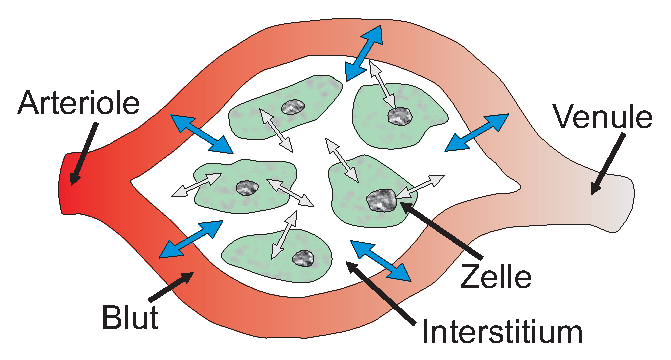
\includegraphics[width=190mm]{images/beispiel1}\vspace{10pt}

\iffalse
\AddToShipoutPicture*{
     \parbox[b][\paperheight]{\paperwidth}{%       
       \vfill
        \centering
        \begin{tikzpicture}[overlay]%
       		  %\draw[help lines] (0,0) grid (10,20);
            \node (0,0) [opacity=0.4]{%
             \hspace{-8,25mm}\includegraphics[width=10cm, height=10cm,keepaspectratio]{\doctitlepic}};%
         \end{tikzpicture}
       \vspace{32.35em}
     }}
\fi






\renewcommand{\arraystretch}{1.3}
\hspace*{-1.8em}
\begin{tabularx}{19cm}{Xl}
\multicolumn{2}{l}{\colorbox{rwthblue}{\hspace{18.4cm}}}\\
\multicolumn{2}{l}{\textsf{\textbf{Chair for Medical Information Technology}}}\\
\multicolumn{2}{l}{\textsf{{Faculty of Electrical Engineering and Information Technology, RWTH Aachen University}}}\\
\multicolumn{2}{l}{\textsf{Univ.-Prof. Dr.-Ing. Dr. med. Steffen Leonhardt}}\\
\textsf{Supervisor: \docsupervisor} & \\ 
\textsf{Date: \today} & \multirow{-2}*~%{
\includegraphics[height=30pt]{images/medit_l_m_blau_meditheadfoot}} \\
\end{tabularx}%}
\renewcommand{\arraystretch}{\defaultarraystretch}

\thispagestyle{empty}
\cleardoublepage

\end{titlepage}

%\include{titelseite_alt}
\cleardoubleemptypage


%**************
%* Danksagung *
%**************

\chapter{Acknowledgments}
\thispagestyle{empty}

Lorem ipsum dolor sit amet, consetetur sadipscing elitr, sed diam nonumy eirmod tempor invidunt ut labore et dolore magna aliquyam erat, sed diam voluptua. At vero eos et accusam et justo duo dolores et ea rebum. Stet clita kasd gubergren, no sea takimata sanctus est Lorem ipsum dolor sit amet. Lorem ipsum dolor sit amet, consetetur sadipscing elitr, sed diam nonumy eirmod tempor invidunt ut labore et dolore magna aliquyam erat, sed diam voluptua. At vero eos et accusam et justo duo dolores et ea rebum. Stet clita kasd gubergren, no sea takimata sanctus est Lorem ipsum dolor sit amet. Lorem ipsum dolor sit amet, consetetur sadipscing elitr, sed diam nonumy eirmod tempor invidunt ut labore et dolore magna aliquyam erat, sed diam voluptua. At vero eos et accusam et justo duo dolores et ea rebum. Stet clita kasd gubergren, no sea takimata sanctus est Lorem ipsum dolor sit amet. 

Duis autem vel eum iriure dolor in hendrerit in vulputate velit esse molestie consequat, vel illum dolore eu feugiat nulla facilisis at vero eros et accumsan et iusto odio dignissim qui blandit praesent luptatum zzril delenit augue duis dolore te feugait nulla facilisi. Lorem ipsum dolor sit amet, consectetuer adipiscing elit, sed diam nonummy nibh euismod tincidunt ut laoreet dolore magna aliquam erat volutpat. 

Ut wisi enim ad minim veniam, quis nostrud exerci tation ullamcorper suscipit lobortis nisl ut aliquip ex ea commodo consequat. Duis autem vel eum iriure dolor in hendrerit in vulputate velit esse molestie consequat, vel illum dolore eu feugiat nulla facilisis at vero eros et accumsan et iusto odio dignissim qui blandit praesent luptatum zzril delenit augue duis dolore te feugait nulla facilisi. 
\cleardoubleemptypage

%************************************************
%* Erkl�rung (hier muss nichts ge�ndert werden) *
%************************************************

%\chapter*{Erkl�rung}
%\thispagestyle{empty}
%\hypertarget{hypsec:erklaerung_der_selbstst}{}%
%
%Ich versichere hiermit, dass ich die vorliegende Arbeit selbstst�ndig
%und ohne Benutzung anderer als der angegebenen Hilfsmittel angefertigt
%habe. Alle Stellen, die w�rtlich oder sinngem�� aus
%ver�ffentlichten und nicht ver�ffentlichten Schriften entnommen
%sind, wurden als solche kenntlich gemacht.\\[3cm]
%
%\begin{tabularx}{\textwidth}{lXl}
%  \rule{5cm}{0.4pt} & & \rule{5cm}{0.4pt}\\
%  Ort, Datum & & Unterschrift
%\end{tabularx}
%\includepdf[angle=90,landscape]{Testbild.png}
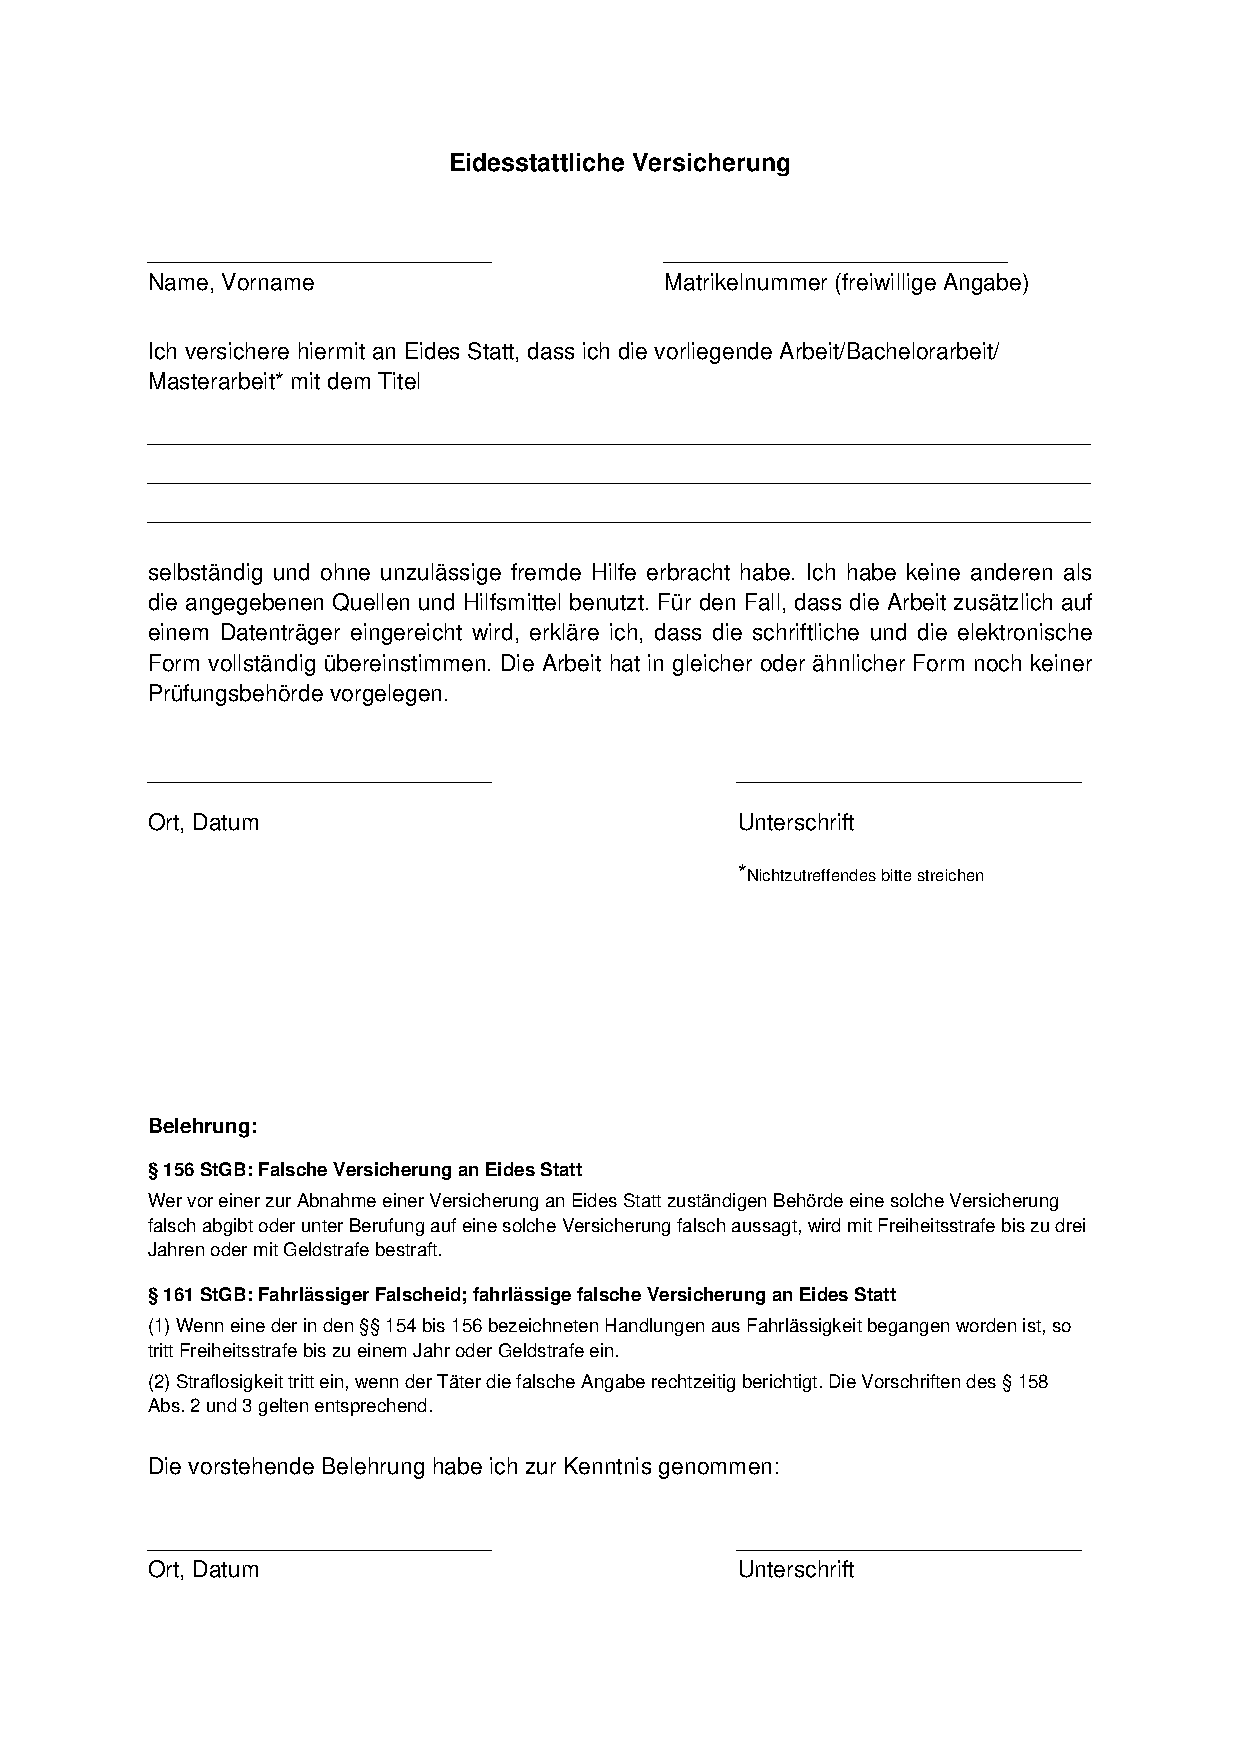
\includepdf{images/Formular_Eidesstattliche_Versicherung_neu}

%\begin{figure}[!ht]
%  \centering
%   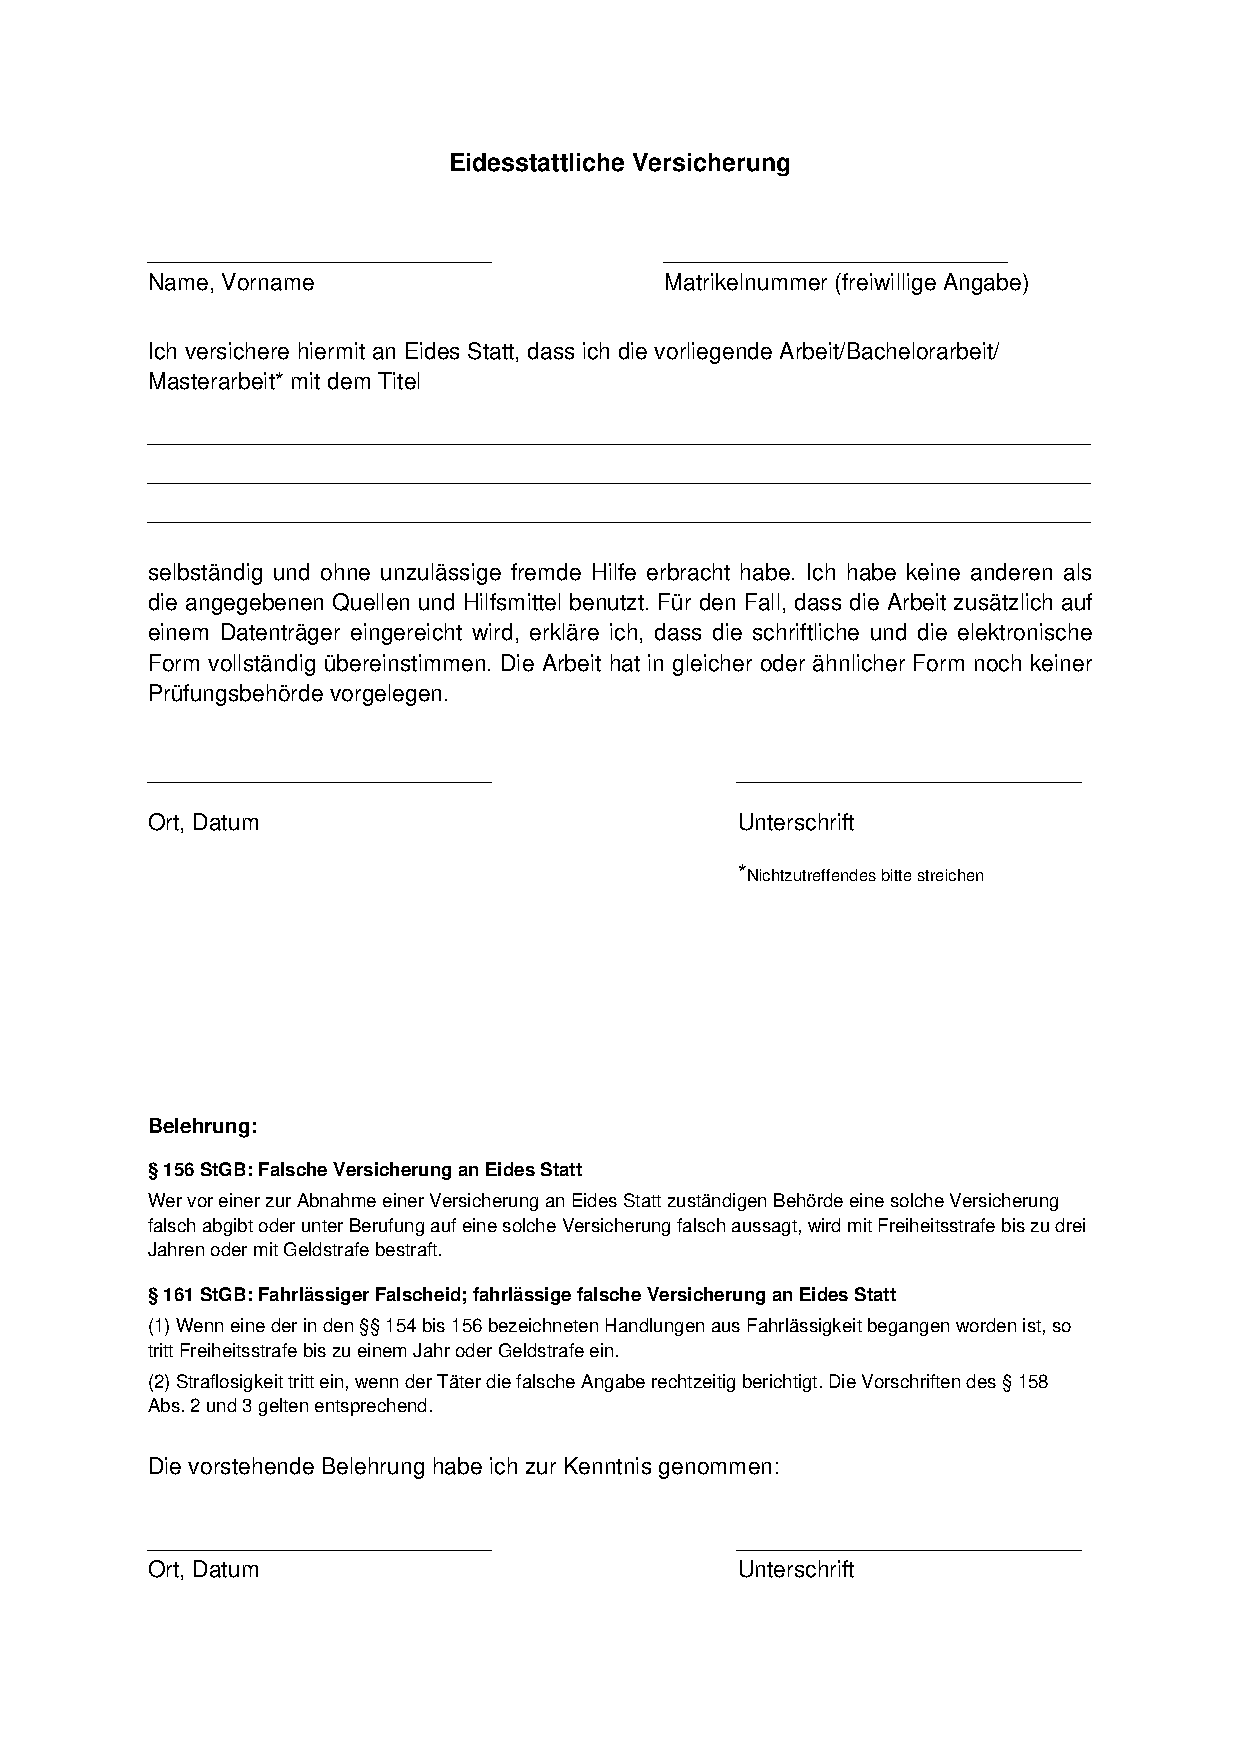
\includegraphics[scale=1]{images/Formular_Eidesstattliche_Versicherung_neu}
%   % Die folgende Anweisungen bindet die Grafik nocheinmal zus�tzlich
%   % als Dateianhang ein. Das hat den Vorteil, dass sie einfach aus dem pdf zur
%   % wieterverwendung extrahierbar ist und der Autor (author) mit angegeben
%   % werden kann. Leider ist die Grafik dadurch auch gleich zweimal im pdf
%   % enthalten und verbraucht dadurch doppelt Platz.
%   % \textattachfile[mimetype=application/pdf,print=false,author=\docauthor,description=\figurename~\ref{fig:beispiel1}]{beispiel1.pdf}{}
%  %% Reihenfolge der Befehle wichtig: zuerst die \caption, danach das \label
%  \label{fig:EidesstattlicheVersicherung}
%\end{figure}

\cleardoubleemptypage

%************
%* Abstract *
%************

\chapter{Abstract}



\cleardoubleemptypage
\thispagestyle{empty}
\cleardoubleemptypage

%**********************
%* Inhaltsverzeichnis *
%**********************

\renewcommand{\contentsname}{Table of Contents}
\addcontentsline{toc}{chapter}{Table of Contents} % Eintrag im Inhaltsverzeichnis erstellen
\tableofcontents                        % Inhaltsverzeichnis anlegen

\renewcommand{\listfigurename}{List of Figures}
\addcontentsline{tof}{chapter}{Table of Figures and Tables}
\listoffigures
\renewcommand{\listtablename}{List of Tables}
\listoftables

\cleardoubleemptypage



%*********************
%* Symbolverzeichnis *
%********************

\chapter*{Symbols}										% da *-Variante m�ssen Kopfzeilen und TOC-Eintrag von Hand generiert werden
\markboth{Symbolverzeichnis}{Symbolverzeichnis} 				% Kopfzeile manuell anpassen 
\addcontentsline{toc}{chapter}{Symbolverzeichnis}				% TOC-Eintrag


\section{Abbreviations}

\begin{tabularx}{\textwidth}{p{.18\textwidth}X}
	AV & Atrioventricular \\
	ANN & Artificial Neural Network \\
	CNN & Convolutional Neural Network \\
	DWT & Discrete Wavelet Transform \\
	ECG & Electrocardiogram \\
	FFT & Fast Fourier Transfrom \\
	HRC & Heart Rate Variability \\
	LBBB & Left Bundle Branch Block \\
	PVC & Premature Ventricular Contraction \\
	RBBB & Right Bundle Branch Block \\
	RMSE & Root Mean Square Error \\
	RT & Repolarization Time\\
	SA & Sinoatrial \\
	WT & Wavelet Transform \\
\end{tabularx}

\cleardoubleemptypage

\mainmatter							% Arabische Nummerierung, Beginn des Hauptteils


%**************
%* Introduction *
%**************

\chapter{Introduction}

Around one billion people travel on airlines annually \cite{PMC2577402}, \cite{aerospace2003medical}. It has also been predicted that the number will be doubled in two decades. During a flight, emergencies occur at a rate of 20 to 100 per million passengers. Many of the cases are not even on the record as there is no proper reporting system. The most common in-flight complaints relate to respiratory, cardiac, traumatic or gastrointestinal related cases. Out of these, cardiac and respiration related complaints are the most serious. During in-flight medical emergencies, a doctor is present only 30 to 60 percent of the time \cite{PMC2577402}, \cite{PMC1119071}. This number may have changed as the article was published in 2008.


\section{Motivation}

Environmental changes such as the rising of altitude, the level of oxygen gradually decreases as the air weakens, including the reduction of atmospheric pressure, temperature, and humidity. As a result, the heart rate increases as it tries to deliver more oxygen to the muscles, which can lead to fainting or even heart attacks among some passenger.

It is important to realize that the on-board medical resources are limited. Therefore, a technological advancement is required, which can reduce the workload of doctors during a flight. Healthcare is one of the hottest research areas in this era. Monitoring of vital signs, parameter, like respiration, ECG, EEG, temperature, and heart rate are of great importance.

A variety of technologies are already available for measuring the vital signs \cite{naturectlesshcs}. They include traditional stethoscopes, electrodes for measuring ECG, and different types of gauges, but they have their drawbacks in terms of comfort and convenience. For example, to measure the ECG, the electrodes are required to be directly attached to the skin of a patient, which is very inconvenient and limits the patient's movement. Blood pressure measurement using Sphygmomanometer that uses belts or cuffs to measure the blood pressure, which again limits the daily activities. Even though these technologies are reliable and provide better results, but they are inadequate for long-term everyday activities.

Contactless sensors are the next big topic in the healthcare. Multiple vital signs can be measured with these sensors without any need of direct contact with the body. They are designed in such a way that they can be integrated into the daily surroundings without any disruption. Different techniques have been used to integrate contact-less sensors into bathtubs \cite{lim2004ecg}, chairs \cite{aleksandrowicz2007wireless}, smartwatches, smartphones, toilet seats \cite{kim2004electrically}, and beds \cite{wu2008contactless} to measure different vital signs. 

The distributed computing, streaming analytics, and machine learning have become more powerful, cheaper, and faster \cite{maprmliotmed}, and they can be applied in various industries:

\begin{itemize}
	\item Healthcare
	\item Transportation
	\item Automobile
	\item Manufacturing
	\item Retail
\end{itemize}


The combination of streaming data, big data analysis, and machine learning can benefit healthcare for identifying chronic diseases such as cardiac disease. Vital signs of the patient can also be analyzed in real-time. The integration of contactless sensor, and deep learning technologies can be used to identify the cardiac arrhythmias in a real-time environment during the flight.

\section{Literature Review}

Variety of methods and devices are available to measure vital signs. The majority of these contributions based on direct contact with the skin. Jeong et al. \cite{jeong2005continuous} measures the blood pressure. They measure the pulse wave using a PPG sensor, which was attached to the earlobe, and an ECG monitoring device with electrodes. Usually electrodes are used to measure the signals from the human body \cite{shen2007detection}, \cite{neuman1998biopotential}.

Many attempts have been made to use sensors that do not require direct contact with the body, but still, they depend on dry electrodes which do not require gel. Jin-Chern Chiou et al. in their study \cite{4600301} showed that how they used the fabricated dry electrodes to measure the EEG signal. Their results showed that dry electrodes perform comparably to the conventional electrodes, but the problem with this approach is that they are limited to only specific areas of the body with no hair where the contact is good.

In the last few years, contactless sensors have gained popularity and have been conspired to measure the signals. Thomas et al. \cite{sullivan2007low} presented a gel-free, non-contact ECG/EEG sensor that capacitively coupled to the skin and can operate up to 3mm distance to the skin. Professor S. Leonhardt \cite{aleksandrowicz2007wireless} described a technique to measure the ECG signal using capacitive coupled electrodes, integrated into an office chair. The signal was measured through a shirt without any direct contact with the skin. Kin-fai Wu et al. \cite{wu2008contactless} in their work proposed a heart rate monitoring system based on a bed, which used contactless electrodes to measure the ECG signal. The design is based on a bedsheet, which is made up of highly conductive material, together with a separate measuring device, which can measure the ECG signal of a lying subject through clothes. 

Electronics company muRata have created under-the-bed sensor  \cite{muratabcg bed}. The sensor uses BCG principle and uses an accelerometer to capture the micro movements caused by respiration and heart. The sensor can measure heart rate, respiration rate, heart rate variability and stroke volume.

Yong Kyu Lim et al. \cite{lim2004ecg} measured the ECG signal using insulated electrodes. The electrodes were attached to the bathtub on both sides of the chest. The recorded signal in their study was noisier as compared to the conventional electrodes signal. But the R peaks were large enough to be detected, which can help to get various vital signs. Yong Kyu Lim et al. in their another study \cite{kim2004electrically} measured the ECG signal on a toilet seat. The capacitive coupled electrodes were used that was insulated on a toilet seat.

Many researchers have used previously traditional machine learning techniques to classify the ECG signals, but the problem with that approach is that the model depends on the researcher's understanding of the data, which is a huge burden. Recent advancement in deep learning techniques has attracted the researchers to implement these techniques in the healthcare.

In 2016 Jun et al. \cite{7838258} proposed a deep neural network to recognize premature ventricular contraction (PVC) beats in an ECG signal. A deep neural network with 6 hidden layers was trained using the TensorFlow library to classify PVC and normal ECG signals. Pourbabaee et al. \cite{7727866} trained a deep convolutional neural network to classify the normal ECG signals with paroxysmal atrial fibrillation (PAF).

In the above both studies, the deep neural network can only classify two different ECG signals. Isin et al. \cite{Isin2017268} used a transferred deep convolutional neural network to classify three different types of ECG signals. In their study, they have used a deep learning framework AlexNet (Krizhevsky et al., 2012) that was previously trained on the general image dataset to carry out the classification of ECG signals. 

\section{Aim}

The aim of this thesis is to build a software system that provides a healthcare solution, which would be able to track various vital signs such as heart rate, temperature, and ECG. Moreover, it should be able to detect the cardiac arrhythmias in real-time with a deep learning model.

The non-contact multi-sensors system consists of the following sensors:


\begin{enumerate}
	\item Capacitive ECG sensor
	\item Photoplethysmogram sensor
	\item Magnetic impedance sensor
	\item Ballistocardiogram sensor
	\item Thermal camera
\end{enumerate}


There can be many use cases where this system can be implemented such as trains, buses, and cars. The use case which is focused in this thesis is the aircraft where the vital parameters of the pilot can be measured.

This system is integrated with non-contact multi-sensors in order to monitor the vital parameters and cardiac related conditions of a pilot during the course of a flight. The early identification of the disease can help to provide a proper treatment to the pilot, as well as can stop from reaching any dangerous situation.

An arrhythmia can be harmless or life threatening. Therefore, for a pilot, a thorough medical evaluation is necessary to assess the severity of arrhythmia for the safety of both pilots and the passengers.

A deep learning model has been designed based on a convolutional neural network in order to detect the cardiac conditions in real-time. The model can detect 4 different types of ECG signals. Various cardiac arrhythmia datasets have taken from the existing dataset. The advantage of using CNN is that, unlike other machine learning algorithms, it does not require a feature extraction phase.

Multiple platforms have been used along with tablets to visualize the results in hand in real-time. A cloud has been set up to store all the sensors data and vital parameters so the data can be accessed from anywhere in the world. The sensor's data can also be used for different purposes such as for the re-training of the deep learning model.


\section{Objective}

The objectives of this thesis are as follow:

\begin{itemize}
	\item Programming of a software visualization (cECG, MI, BKG, and PPG) for a PC along with the tablet notification and visualization
	\item Construction of the data bank on the cloud
	\item Preprocessing of the signals and feature extraction
	\item Arrhythmia data collection
	\item Deep learning of the cardiac conditions
	\item Evaluation of the algorithm with real-time data from the non-contact multi-sensors system
\end{itemize}




%**************
%* Background *
%**************

\chapter{Introduction}


\section{Anatomy of Heart}
The function of the heart is to pump the blood inside the body, which is stimulated by an electrical stimulus \cite{wilkins2005ecg} \cite{electric_activity_heart}. The heart pumps blood through the arteries, veins to the different parts of the body such as organs, muscles, and tissues.

The heart is made up of 4 chambers, left and right atria, and left and right ventricles, as can be seen in Figure ~\ref{fig:heart_anatomy}. The right atrium receives de-oxygenated blood from the whole body and pumps it into the right ventricle which then pumps the blood to the lungs for oxygenation. The left atrium receives oxygenated blood from the lungs and pumps it into the left ventricles which then pumps the oxygenated blood to the whole body. The aorta carries oxygenated blood to the different part of the body and the pulmonary arteries carry the de-oxygenated blood back to the lungs for oxygenation. The important point to note here is that the blood flows to different organs via arteries and returns back to the heart via veins.

The main components of the cardiac conduction system are:
\begin{enumerate}
	\item Synoatrial (SA) Node
	\item The Atrioventricular (AV) Node
	\item Atrioventricular (AV) Bundle or Bundle of His
	\item Right and Left Bundle Branches
	\item Purkinje Fibers
\end{enumerate}


\begin{figure}[htpb]
	\centering
	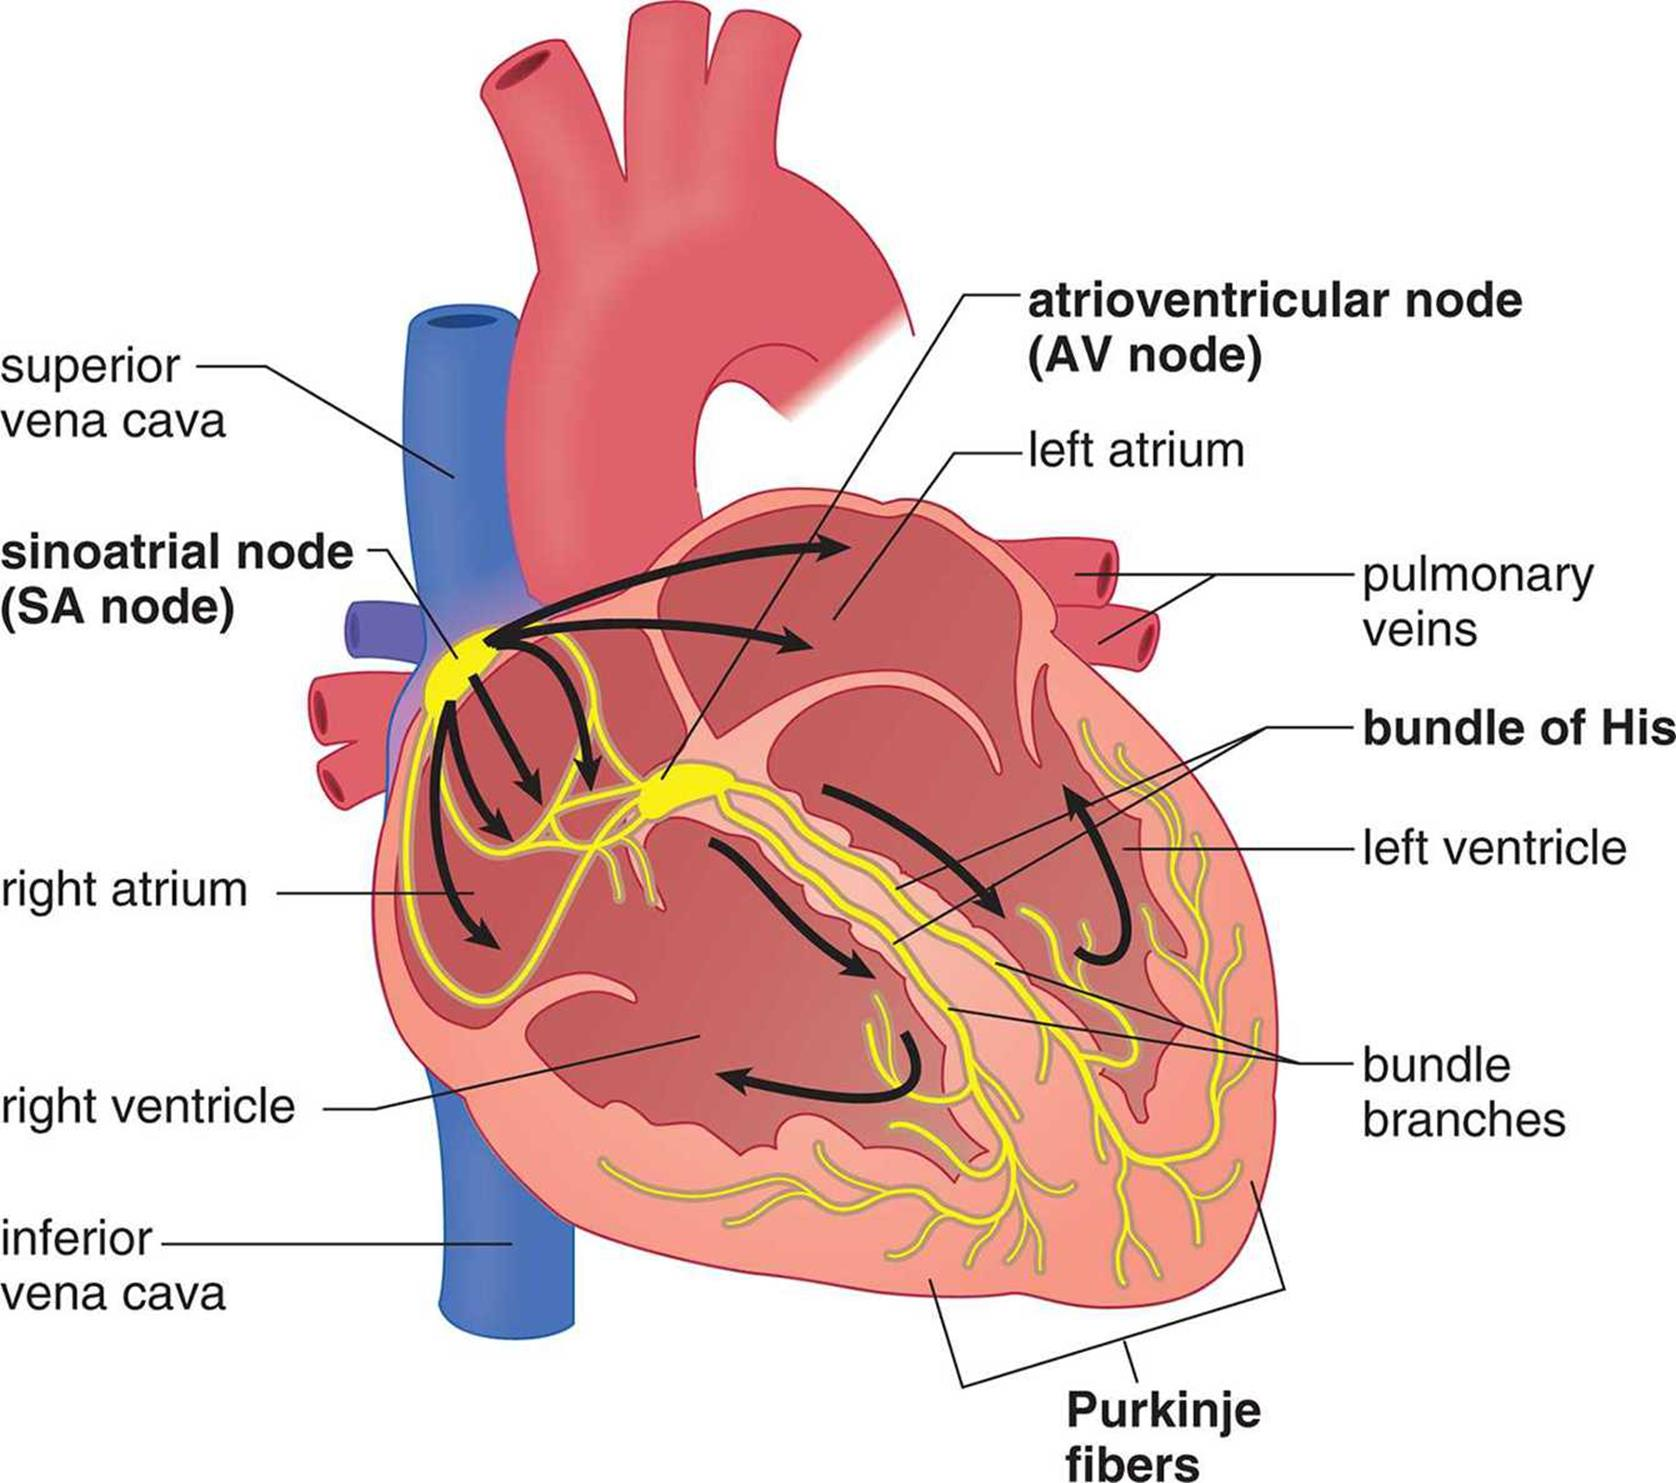
\includegraphics[width=\textwidth,height=7cm,keepaspectratio=true]{images/electric_activity_heart}
	\caption{
		The electrical activity of heart, taken from \cite{electric_activity_heart}.
	}
	\label{fig:heart_anatomy}
\end{figure}




The SA node, also known as sinus node, is a natural pacemaker of the heart which is located in the right atrium. It produces an electric stimulus at the rate of 60 to 100 signals per minute (under normal condition), which travels through the heart to make it pump the blood to the body. It initiates all heartbeats and determines the heart rate. The electrical impulse from the SA node spread throughout the atrium which results in the contraction of the atrium. The AV node which is located on the other side of the right atrium, near the AV valve, serve as a gateway to the ventricles. It also delays the passage of electrical impulse to the ventricles. It is to ensure that, all the blood is ejected from the atria to the ventricles before the ventricles contract. The AV node then passes the signal to the atrioventricular (AV) bundle or bundle of His. The bundle is divided into two parts, right and left bundle branches to stimulate the right and left ventricles. The signal then travels down to the Purkinje fibers where from the signal spreads upwards throughout the ventricular myocardium. Each contraction of the ventricles represents one single heartbeat.

Each heartbeat is composed of two phases, known as systole and diastole. During \textbf{systole}, the heart muscles contract and the blood is pumped from ventricles to the different parts of the body. During \textbf{diastole}, the hearts muscles relax and the blood from atria flows into the ventricles. The pressure generated during systole from the ventricular contraction is high, whereas, during diastole, the muscle relaxation reduces this pressure.

The electrical activity of the heart can be detected in the form of Electrocardiogram by placing electrodes on the body surface. It is a powerful tool for diagnosing the status of patient's heart.



\section{The Electrocardiogram} \label{the_electrocardiogram}

Electrocardiogram (ECG) is an essential tool for diagnosing the electrical activity of the heart \cite{wilkins2005ecg}. It is a simple, non-invasive procedure to measure the activity of the heart. Most of the tools available today to measure the ECG are based on the electrodes which are required to be attached to the body. The electrodes sense the electrical currents inside the body and transmit them to the ECG monitor. These currents are then transformed into appropriate waveforms which represent the heart's polarization and depolarization cycle. Different components of the wave represent the activity of different parts of the heart.


In conventional 12-lead ECG, 10 electrodes or leads are attached to the patient's body and then the electrical activity of the heart is viewed from 12 different perspectives \cite{cablesandsensors}. These 12 views of the heart are captured by placing the electrodes on chest, wrists, and ankles. The main purpose of ECG is to identify any cardiac arrhythmia, ischemia, problems with heart rate or irregularities.

These 10 electrodes are divided into 2 groups. 
\begin{enumerate}
	\item 6 chest electrodes
	\item 4 limb electrodes
\end{enumerate}

\begin{figure}[htpb]
	\centering
	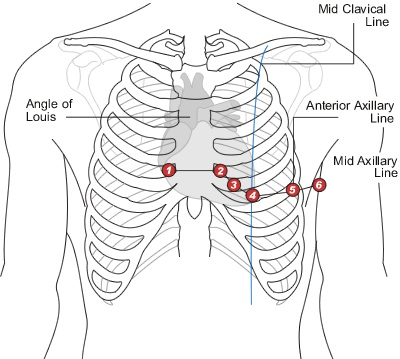
\includegraphics[width=\textwidth,height=6cm,keepaspectratio=true]{images/6_lead_placement}
	\caption{
		The leads position on chest, taken from \cite{TUON:six_leads}.
	}
	\label{fig:6_lead_placement}
\end{figure}


\subsubsection{Chest Electrodes}
The chest electrodes are denoted as ``V'' and they all are numbered from V1 to V6 as can be seen in Figure ~\ref{fig:6_lead_placement}. The electrodes are positioned at the following locations on the chest:

\begin{itemize}
	\item V1 - Fourth intercostal space (between ribs 4 and 5) on the right sternum
	\item V2 - Fourth intercostal space (between ribs 4 and 5) on the left sternum
	\item V3 - Placed in the middle of V2 and V4
	\item V4 - Fifth intercostal space (between ribs 5 and 6) at the mid-clavicular line
	\item V5 - Placed horizontally on anterior axillary line with V4
	\item V6 - Placed horizontally on Mid-axillary line with V4 and V5
\end{itemize} 


The 3 different axillary lines \textbf{anterior axillary line}, \textbf{midaxillary line}, and \textbf{posterior axillary line} can be seen in Figure ~\ref{fig:axillary_lines}. 

\begin{figure}[htpb]
	\centering
	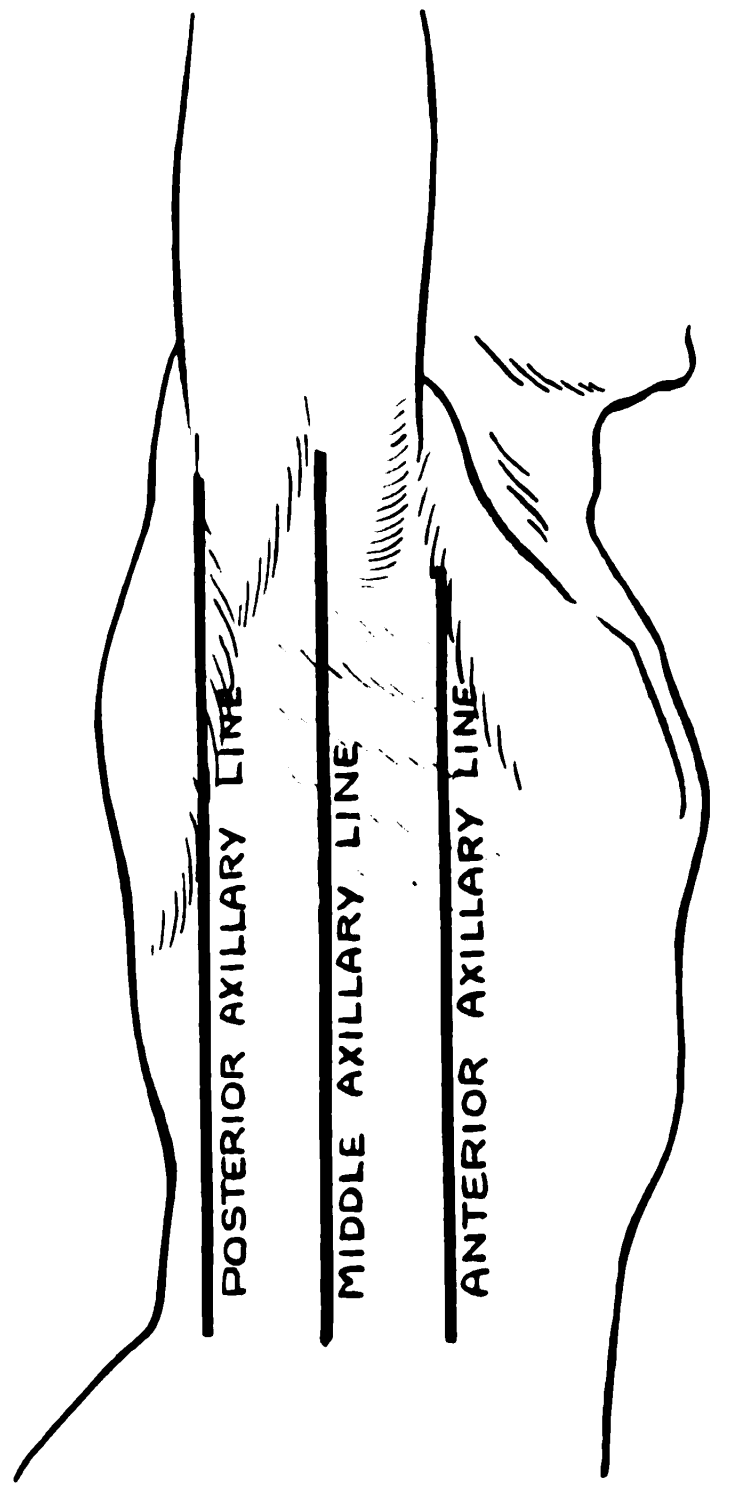
\includegraphics[width=\textwidth,height=6cm,keepaspectratio=true]{images/Brantigan_1963_1-53.png}
	\caption{
		The axillary lines on the right side of chest, taken from \cite{wiki:aux_lines}.
	}
	\label{fig:axillary_lines}
\end{figure}



\subsubsection{Limb Electrodes}
The 4 limb electrodes are denoted as RA, LA, LL, RL and there respective positions are:

\begin{itemize}
	\item RA - Anywhere on right arm between shoulder and elbow, but avoiding thick muscles.
	\item LA - Symmetric to the RA position, but on left arm
	\item RL - Anywhere on right leg between the torso and the ankle
	\item LL - Symmetric to the RL position, but on left leg
\end{itemize} 

The limb electrodes are shown in Figure ~\ref{fig:limb_leads}

\begin{figure}[htpb]
	\centering
	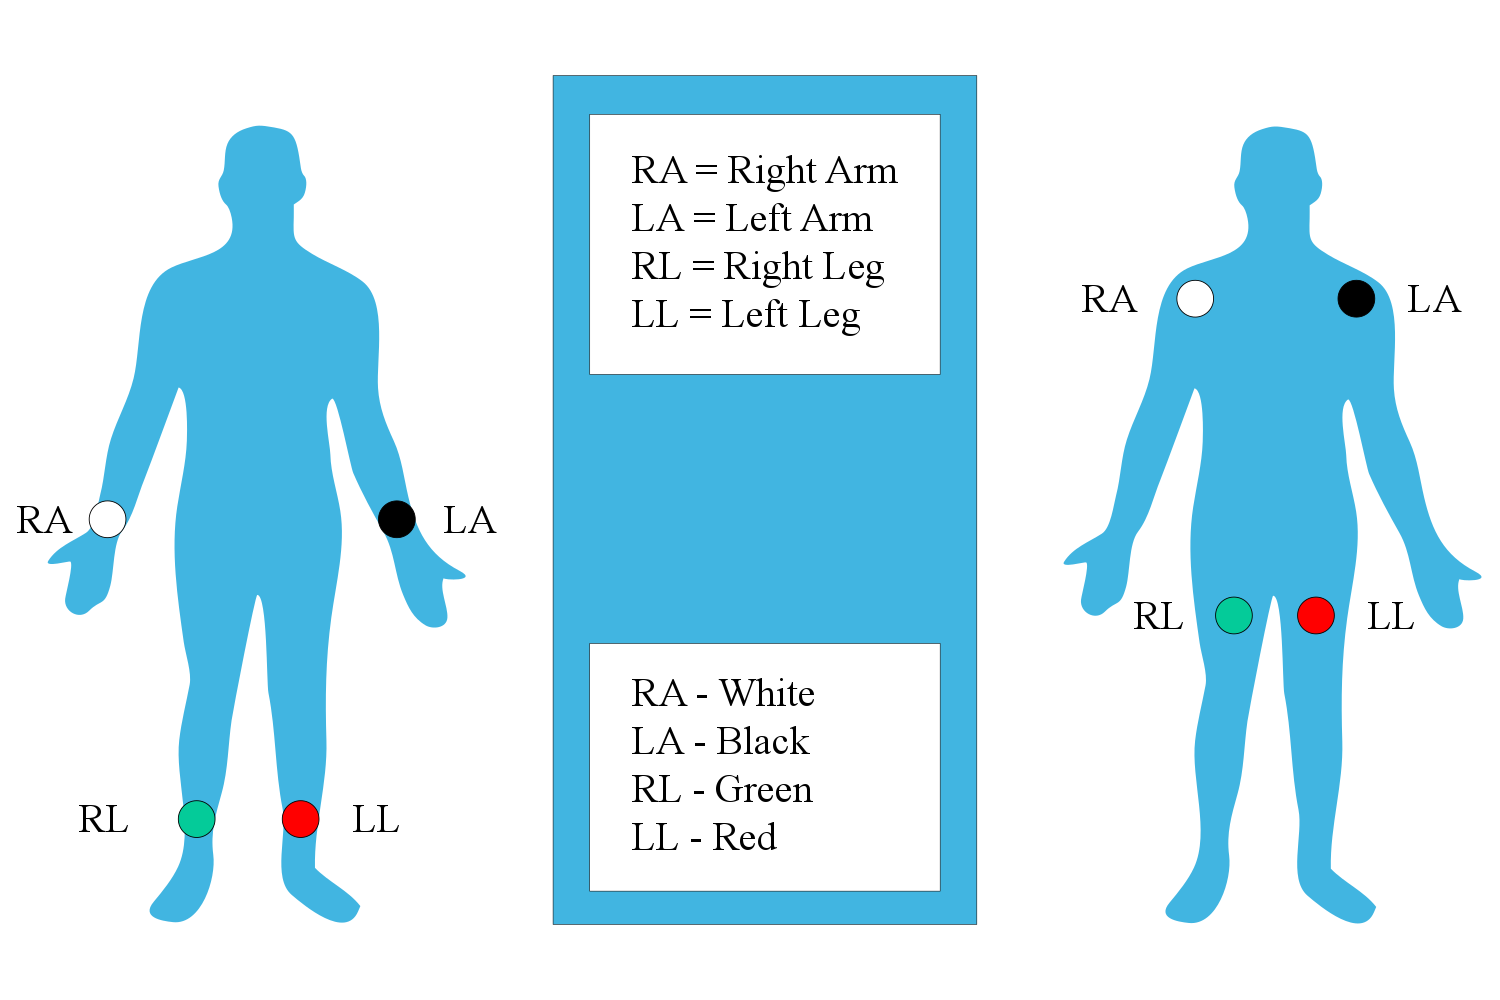
\includegraphics[width=\textwidth,height=6cm,keepaspectratio=true]{images/Limb_leads}
	\caption{
		The possible position of limb leads, taken from \cite{wiki:limb_leads}.
	}
	\label{fig:limb_leads}
\end{figure}


\section{ECG Complex}
ECG complex represents the electrical activity of the heart during one cardiac cycle \cite{wilkins2005ecg}. A normal cardiac cycle consists of five waveforms labeled with P, Q, R, S and T as can be seen in Figure ~\ref{fig:SinusRhythmLabels}. The Q, R and S waves are referred to as one unit, the QRS complex. The ECG signal represents the conduction of electrical impulses from the atria to the ventricles. The important parameters in the ECG signal are:

\subsection{P Wave}

The P wave is the first component of the ECG signal. It occurs due to contraction of both left and right atrium. This process is also known as atrial depolarization. A normal P wave has following characteristics (in lead II):
\begin{itemize}
	\item duration: 0.06 to 0.12 seconds
	\item amplitude: 2 to 3 mm high
	\item location: before the QRS complex
\end{itemize}

\begin{figure}[htpb]
	\centering
	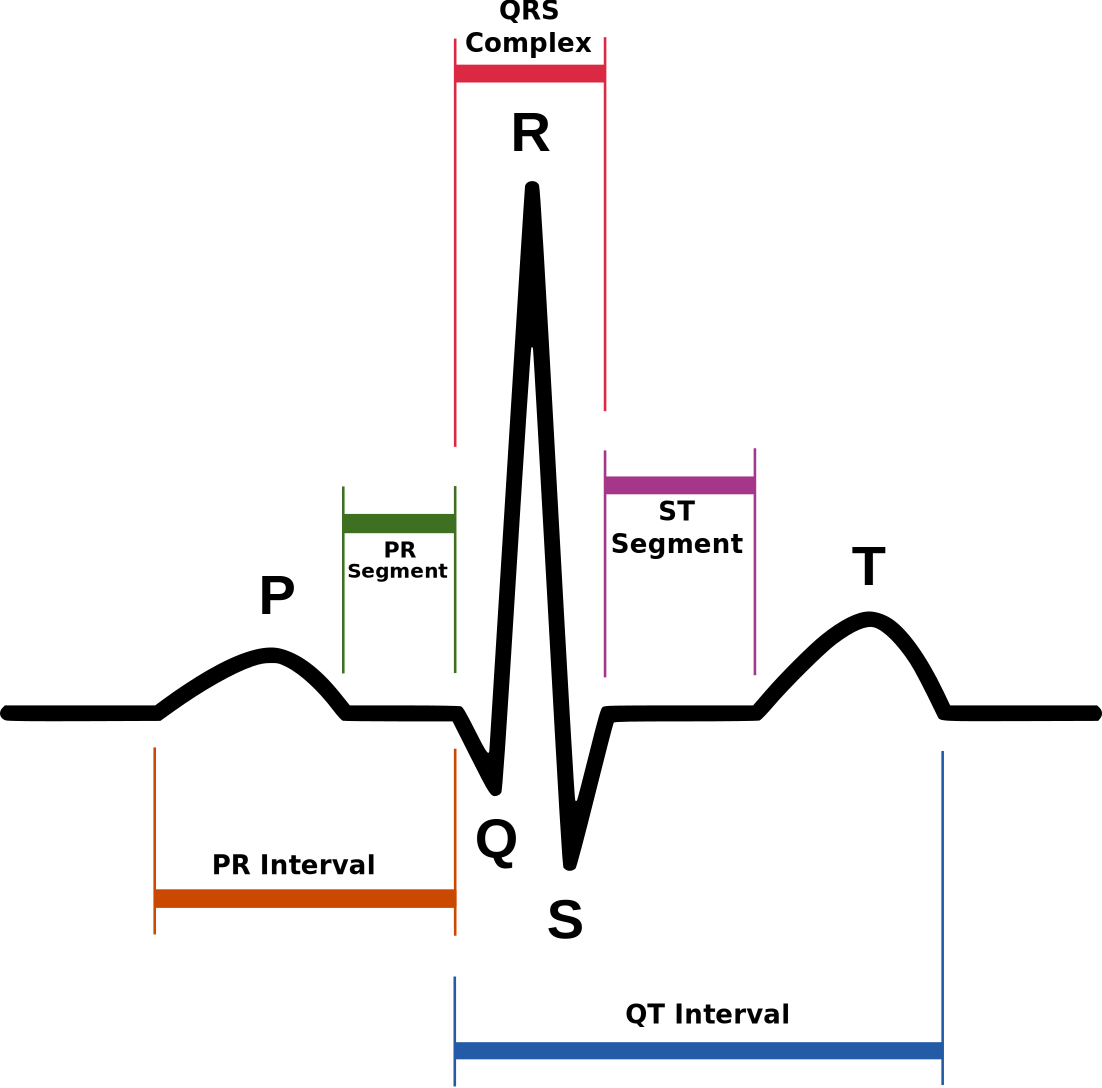
\includegraphics[width=\textwidth,height=6cm,keepaspectratio=true]{images/SinusRhythmLabels}
	\caption{
		The ECG signal, taken from \cite{wiki:SinusRhythmLabels}.
	}
	\label{fig:SinusRhythmLabels}
\end{figure}

\subsection{QRS Complex}
The QRS complex follows the P wave and represents a contraction of both right and left ventricles. This contraction results in the blood ejection from the heart which eventually pumps into the arteries, creating a pulse. The Q and S waves are relatively very small whereas, R wave is comparatively very big. A normal QRS complex has following characteristics (in lead II):

\begin{itemize}
	\item duration: 0.06 to 0.10 seconds
	\item amplitude: 5 to 30 mm high
	\item location: follows the P wave
\end{itemize}

\subsection{T Wave}
The T wave represents the ventricles re-polarization. It occurs during the last part of ventricle systole. The T wave has following characteristics (in lead II):

\begin{itemize}
	\item duration: 0.10 to 0.25 seconds or greater
	\item amplitude: <5 mm high
	\item location: follows the QRS complex
\end{itemize}

\subsection{PR Interval}
The PR interval is the time interval between the end of contraction of the atrium and beginning the contraction of the ventricles. A normal PR interval has following characteristics:

\begin{itemize}
	\item duration: 0.12 to 0.20 seconds
	\item location: From the beginning of P wave to the beginning of the QRS complex
\end{itemize}

\subsection{ST Segment}
The ST segment represents the end of ventricular depolarization and the beginning of the ventricles relaxation. The Point between the end of QRS complex and the beginning of ST segment is called as the J point. A normal ST segment has following characteristics:

\begin{itemize}
	\item duration: 0.08 to 0.12 seconds
	\item location: From the end of QRS complex to the beginning of T wave
\end{itemize}

\subsection{QT Interval}
The QT interval is the time interval between the ventricular depolarization and repolarization. The QT duration varies according to the heart rate. Faster heart rate results in smaller QT interval whereas, slower heart rate may result in bigger QT interval. The bigger QT interval may result in an irregular heartbeat. A normal QT interval has following characteristics:

\begin{itemize}
	\item duration: 0.36 to 0.44 seconds
	\item location: From the beginning of QRS complex to the end of T wave
\end{itemize}

\section{Disadvantages of Attached Electrodes} \label{electrodes_disadv}

While it is easy to monitor the electrical heart activity by placing the electrodes directly on the body but it has several disadvantages as well.

\begin{itemize}
	\item It limits the patient's mobility.
	\item Discomfort for the patient as electrodes are directly attached to the body.
	\item Loss of cardiac monitoring in case if patient moves.
	\item Long contact of the electrodes may irritate the skin.
\end{itemize}

\section{Noise in ECG Signal}
Most of the time, the ECG signal is corrupted by the different types of noises and artifacts which changes the characteristics of the ECG signal \cite{limaye2016ecg}. Hence, it becomes very difficult to extract the useful information from the signal. Following are the major noises which are present in the ECG signal.

\subsection{Power Line Interference}
Power line interference is a 60 Hz noise which is present in ECG signal because of the improper grounding of the ECG equipment or interference from the nearby equipment. In order to remove this type of noise, a proper use of a filter is required. A 60 Hz notch filter can be used to remove the power line interference. Figure ~\ref{fig:ACInterference} illustrates the 60 Hz power line interference in ECG signal.

\begin{figure}[htpb]
	\centering
	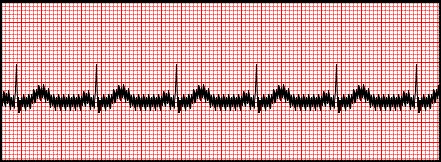
\includegraphics[width=10cm,height=7cm,keepaspectratio=true]{images/ACInterference}
	\caption{
		60 Hz AC Interference, taken from \cite{ecg_artifacts}.
	}
	\label{fig:ACInterference}
\end{figure}

\subsection{Baseline wander}
Baseline wander is a low-frequency component which corrupts the ECG signal because of breathing, body movements, dirty or lose electrodes, electrode impedance, etc. Generally, they have a frequency greater than 1 Hz. A high pass filter can be used to remove the baseline wander. The baseline wandering in ECG signal can be seen in Figure ~\ref{fig:WBaseline}.

\begin{figure}[htpb]
	\centering
	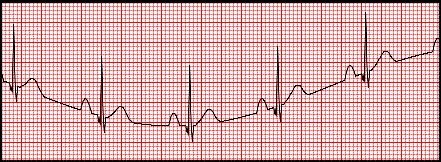
\includegraphics[width=10cm,height=7cm,keepaspectratio=true]{images/WBaseline}
	\caption{
		Baseline wandering in ECG signal, taken from \cite{ecg_artifacts}.
	}
	\label{fig:WBaseline}
\end{figure}

\subsection{Muscle Noise}
This type of noise is caused by muscle contractions besides heart which results in the change of heart electric potential \cite{markovski2013ict}. When the other muscles near the electrodes depolarized and re-polarized, they also generate waves which are then picked up by the ECG. They generally occur in short time burst and have higher amplitude values than the ECG signal. It can be removed using wavelet transform \cite{6091791}. An example of ECG signal affected by muscle contractions can be seen in figure ~\ref{fig:Tremor}.

\begin{figure}[htpb]
	\centering
	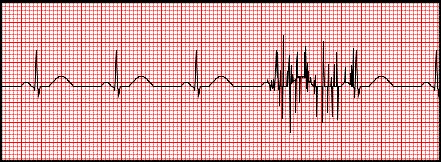
\includegraphics[width=10cm,height=7cm,keepaspectratio=true]{images/Tremor}
	\caption{
		ECG signal combined with muscle noise , taken from \cite{ecg_artifacts}.
	}
	\label{fig:Tremor}
\end{figure}

\section{Arrhythmias}
Irregularity in the heartbeat is known as arrhythmia (also called dysrhythmia) ~\cite{medicinenet}. During an arrhythmia, a heart is out of normal rhythm and may feel like the heart has skipped a beat or beat with an irregular pattern. A normal heart rate lies between 60 to 100 beats per minute and arrhythmia can occur with normal heart rate,  slow heart rate (called bradycardia) in which heart rate 
is less than 60 beats per minute or with rapid heart rate (called tachycardia) in which heart beats faster than 100 beats
per minute.



\subsection{Causes of an Arrhythmia}
Arrhytmia can be caused by one of the following reasons:

\begin{itemize}
	\item Heart disease
	\item Electrolyte imbalance
	\item Changes in heart muscle
	\item After surgery effects
\end{itemize}

\subsection{Types of Arrhythmias}

The most common types of arrhythmias are:

\subsubsection{Premature Ventricular Contraction}
It is a type of arrhythmia in which the heartbeat is initiated by the ventricles rather than the SA node. It is generally referred as "skipped beats". This is the most common type of arrhythmia which occurs with or without any heart disease. It could be the result of too much stress, usage of too much cocaine or restless. But sometimes it can also be caused by heart disease. Most of the time PVC is considered as harmless and rarely needs a treatment.

\begin{figure}[htpb]
	\centering
	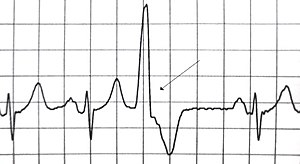
\includegraphics[width=10cm,height=7cm,keepaspectratio=true]{images/pvc}
	\caption{
		Premature Ventricular Contraction, taken from \cite{wiki:pvc}.
	}
	\label{fig:pvc}
\end{figure}

\subsubsection{Atrial Fibrillation}
This type of arrhythmia caused by the abnormal contraction of the upper chamber of the heart. During atrial fibrillation, the atria beat irregularly without any coordination with the ventricles. This could results in heart palpation, shortness of breath and weakness.


\subsubsection{Atrial Flutter}
This type of arrhythmia caused by problems in the heart's electrical system. It is similar to atrial fibrillation but rhythm in atria is more organized than the atrial fibrillation. The risk factors and causes of atrial flutter are similar to those of atrial fibrillation.

\begin{figure}[htpb]
	\centering
	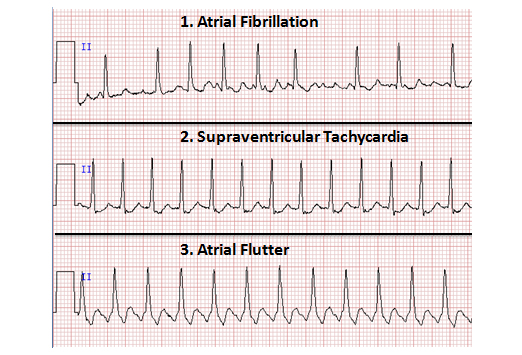
\includegraphics[width=15cm,height=12cm,keepaspectratio=true]{images/af}
	\caption{
		Atrial Fibrillation vs Atrial Flutter vs Tachycardia , taken from \cite{sumdu}.
	}
	\label{fig:af}
\end{figure}


\subsubsection{Bradycardia}
In this type of arrhythmia, the heart beats slower than the normal pace, usually less than 60 beats per minute. This could be because of the disease in electrical heart system.

\subsubsection{Tachycardia}
In this type of arrhythmia, the heart beats faster than the normal pace, usually, more than 100 beats per minute. When the heart beats too fast, it may not pump blood effectively to the body parts, which could result in shortness of breath.

\subsubsection{Heart Block}
In this type of arrhythmia, the heart beats slowly because of the delay or complete block of the electrical signal between the upper chambers and the lower chambers of the heart. It is also called atrial ventricular block (AV block).

\subsubsection{Bundle Branch Block}
Bundle branch block can be of two types, left bundle branch block (LBBB) and right bundle branch block (RBBB). In a normal heart, both bundles depolarized simultaneously and contract at the same time. In this type of arrhythmia, the affected bundle depolarized slowly whereas the un-affected bundle depolarized normally which results in a broader QRS complex, generally longer than 120 milliseconds duration. LBBB and RBBB can be seen in figure ~\ref{fig:LRBBB}.


\begin{figure}[htpb]
	\centering
	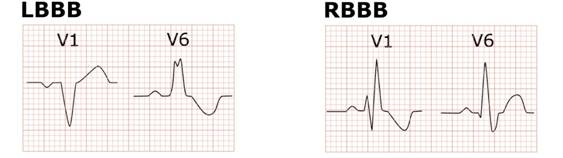
\includegraphics[width=12cm,height=10cm,keepaspectratio=true]{images/LRBBB}
	\caption{
		LBBB vs RBBB , taken from \cite{bilagi}.
	}
	\label{fig:LRBBB}
\end{figure}


%**************
%* ECG Feature extraction *
%**************

%\ihead{\headmark}
\chapter{ECG Signal and Data Processing}


\section{Devices}

Wireless sensor devices and contact-less sensor devices are the current trends in the health informatics. The recent improvements in the sensor devices made it possible for the people to bring this idea
into reality. When  medical sensor devices are combined with cloud computing, it can be thought of as a complete
solution for a health care system which not only can be used
in hospitals but also can be utilized out of the hospital when
the doctor is unreachable regardless of the patient's location.
Doctors will still be able to monitor his patient condition and
according to the patient situation they can instruct the device,
that is, attached to the patient, to take appropriate actions.
One example can be thought of as a person running somewhere and during that he/she feels some heart pain. Sensors assess the patient's condition and immediately send some notification to the doctor. After looking at the conditions, he sends back a response to the devices, which then acts according to the instruction such as, injects some medicine into the patient body. It can also be used to keep track of the patient location so, in the case of emergency, an ambulance can be instructed to go there.
Many of the sensors can be installed in the patient's surrounding, whereas,
several sensors can be wearable. These sensors can monitor
body temperature, respiration, heart rate, blood pressure, ECG, EEG, etc.
Along with sensors, it might be possible that there are several
actuators attached to the patient body which is activated by
certain events such as the rise of sugar level in blood.

Multiple contact-less sensor devices are used to implement a system for the thesis, which collects data of the user and process that in real-time. The following devices are used in the implementation:

\subsection{Magnetic Impedance Sensor}

The magnetic impedance (MI) sensor measures the small changes in electrical resistance of the chest or different regions of the body. It uses special electrodes which emit very low voltage electric current into the body. As the voltage level is very low, therefore, it does not interfere with the heart's electrical system. The MI sensor measures the resistance to the flow of current as it passes through the body via blood, as blood is a good conductor.

During systole, as the blood volume increases, impedance decreases. Similarly, during diastole, the blood volume decreases and the impedance increases.


\begin{figure}%
	\centering
	
	\subfigure[]{%
		\label{fig:ex3-e}%
		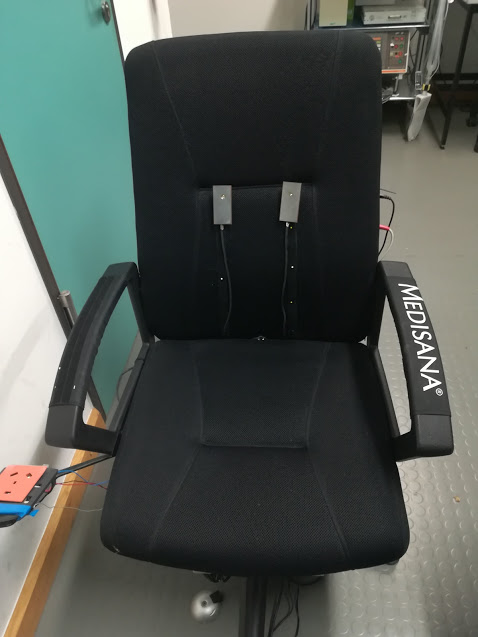
\includegraphics[height=2in]{images/ecg}}%
	\hspace{8pt}%
	\subfigure[][]{%
		\label{fig:ex3-a}%
		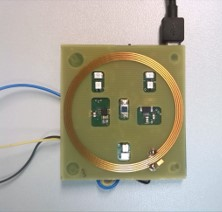
\includegraphics[height=2in]{images/mi}}%
	\hspace{8pt}%
	\subfigure[][]{%
		\label{fig:ex3-b}%
		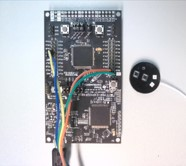
\includegraphics[height=2in]{images/ppg}} \\
	\subfigure[][]{%
		\label{fig:ex3-c}%
		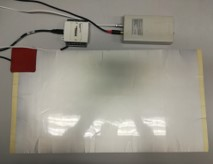
\includegraphics[height=2in]{images/bcg}}%
	\hspace{8pt}%
	\subfigure[][]{%
		\label{fig:ex3-d}%
		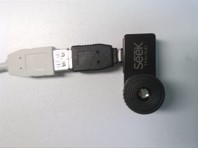
\includegraphics[height=2in]{images/tc}}%
	\caption[A set of sensor devices.]{A set of sensor devices:
		\subref{fig:ex3-e} an ECG sensor;
		\subref{fig:ex3-a} a MI sensor;
		\subref{fig:ex3-b} a PPG sensor;
		\subref{fig:ex3-c} a BCG sensor; and,
		\subref{fig:ex3-d} a thermal camera.}%
	\label{fig:ex3}%
\end{figure}



The MI sensor provides a data packet of 42 bytes, which splits into the attributes shown in table \ref{tab:att_mi}. The byte identifier of the sensor can be seen in the table \ref{tab:bi_mi}.

There is an exception in the data packet when it contains 0x8101 or 0x8102. In this case, the size of the data packet may vary according to the number of count of the corresponding bytes. Moreover, the data packet should be examined and if it contains the corresponding bytes, the data packet should be modified and the bytes 0x8101 should be replaced with 0x81 and 0x8102 should be replaced with 0x82. This modification has been done in order to differentiate it with the header and data packet identifier as they have the same value.


\renewcommand{\arraystretch}{2}
\begin{table}
	\caption{Attributes of MI sensor.} \label{tab:att_mi}
	
	\begin{center}
		\begin{tabular}{ | l | r | }
			\hline
			\textbf{Attributes} & \textbf{Size (Bytes)} \\ \hline
			MI\_RAW  & 4 \\ \hline
			MI  & 4  \\ \hline
			RED\_RAW  & 4  \\ \hline
			ECG\_RAW  & 4  \\ \hline
			IR\_RAW  & 4  \\ \hline
			RED\_AVG  & 4  \\ \hline
			ECG\_AVG  & 4  \\ \hline
			IR\_AVG  & 4  \\ \hline
			ACC\_X  & 2  \\ \hline
			ACC\_Z  & 2  \\ \hline
			ECG\_REF  & 2  \\ \hline
			RESP\_REF  & 2  \\ \hline
			BATTERY  & 2  \\ \hline
		\end{tabular}
	\end{center}
	
\end{table}


\renewcommand{\arraystretch}{2}
\begin{table}
	\caption{Byte identifiers for the MI sensor.} \label{tab:bi_mi}
	
	\begin{center}
		\begin{tabular}{ | l | r | }
			\hline
			\textbf{2-Byte Identifier} & \textbf{Description} \\ \hline
			0x81  & Header \\ \hline
			0x82  & Data Packet  \\ \hline
		\end{tabular}
	\end{center}
	
\end{table}

\subsection{Photoplethysmogram Sensor}
The photoplethysmogram (PPG) sensor is used to measures the variations in blood flow in the body with each heartbeat. A PPG sensor uses a light source to illuminate the blood and a photo-detector to measures the variations in the light intensity associated with changes in the blood volume. The decrease in light intensity indicates the increase in blood volume and increase in light intensity indicates the decrease in blood volume.

The sensor provides the PPG signal with 4 different channels, a temperature, which is measured in Celsius and accelerometer coordinates. The size of the data changes according to the attributes which can be seen in the table \ref{tab:att_ppg}. The frequency of the data packets changes according to the attributes. The temperature value is sent every one second, whereas, the frequency rate of PPG channels is 100 samples per second. Similarly, for the accelerometer coordinates, the data rate is 50 samples per second.

% Please add the following required packages to your document preamble:
% \usepackage{multirow}
\begin{table}[]
	\centering
	\caption{Attributes of PPG sensor.}
	\label{tab:att_ppg}
	\begin{tabular}{|l|l|l|l|}
		\hline
		\textbf{2-Byte Identifier} & \textbf{Attributes} & \textbf{Size (Bytes)} & \textbf{Data} \\ \hline
		\multirow{4}{*}{} 0x0050 & \multirow{4}{*}{} ppg (8 Bytes) & 2 & Channel 1 \\ \cline{3-4} 
		&                   & 2 & Channel 2 \\ \cline{3-4} 
		&                   & 2 & Channel 3 \\ \cline{3-4} 
		&                   & 2 &  Channel 4 \\ \hline
		0x0054 & Temperature (2 Bytes) & 2 & Temperature \\ \hline
		\multirow{3}{*}{} & \multirow{3}{*}{} & 2 & X Coordinate \\ \cline{3-4} 
		0x0041 & Accelerometer coordinates (6 Bytes) & 2 & Y Coordinate \\ \cline{3-4} 
		&  & 2 & Z Coordinate \\ \hline
	\end{tabular}
\end{table}


\subsection{ECG Sensor}
As described in section \ref{the_electrocardiogram}, the ECG signal is usually collected by placing electrodes directly on the body but it has several disadvantages as well, which is described in section \ref{electrodes_disadv}. Therefore, non-contact capacitive electrodes have been used to collect the ECG signals of the person. Unlike traditional electrodes, which rely on galvanic contact, the capacitive electrodes are insulated from skin using a dielectric material, such as, air gap, clothes, etc \cite{bouchard2017smart}. The ECG signal propagates via skin to the dielectric material and then to the electrodes through a capacitive coupling. The major drawback of this approach is that it is very sensitive to body motion.

\subsection{Ballistocardiogram Sensor}
The ballistocardiogram (BCG) sensor measures the ballistic forces associated with cardiac contraction and ejection of blood. These ballistic forces are mainly measures by the electromechanical film (EMFi) sensor which converts the mechanical energy into the electrical signal and vice versa. Most of the time, the EMFi sensing device is placed on a chair or bed, which measures the pressure associated with the cardiac activity.

\subsection{Thermal Camera}
A thermal camera is also used to measures the temperature of the person. A thermal seek camera is used for the implementation which captures the thermo temperature images, from which then the temperature is calculated.

\section{ECG Signal Processing}
QRS complex detection is the basis for processing ECG signal. Regardless of what application is required, the accurate detection of QRS complex is a pre-requisite for feature extraction. In order to detect the QRS complex accurately, it is necessary to detect the R-peak position correctly. Once the QRS complex is identified, further examination of the signal can be performed such as heart rate, arrhythmias, classification of ECG signal, ST segment etc. Moreover, P and T waves can also be extracted.

The ``QRS Complex'' is the combination of Q, R and S waves and it represents the contraction of the ventricles. It plays a significant role in the detection of cardiac arrhythmias.

Many methods have already been proposed for the detection of QRS complex. These methods fall into 3 categories \cite{5639905}.

\begin{enumerate}
	\item Filter Method
	\item Artificial Intelligence Method
	\item Wavelet transform Method
\end{enumerate}

\subsection{Filter Method}
The filter method uses bandpass filter to filter the ECG signal \cite{4122029}\cite{554762}. In this method, a QRS complex is intensified by suppressing the P and T wave. This method is generally very quick and takes less time to implement. But the major drawback of this method is that the frequency band of QRS complex and of noise overlapping, affect its performance.

\subsection{Artificial Intelligence Method}
The detection of QRS complex using this method is fast, accurate and more robust, but in reality, it is very time-consuming and difficult to implement \cite{126604}\cite{PIETKA1991139}\cite{58593}. Therefore, this method is not very popular and not widely used as compared to the other methods.

\subsection{Wavelet Transform Method}
Wavelet transform method becomes very popular in detecting the QRS complex. It is based on time-frequency analysis. It is very efficient and takes less to implement. Many people have already used wavelet transform for detecting the QRS complex. Yazhu Qiu \cite{PMID:17228741} used Mexican-hat wavelet to detect ECG signal. In the proposed method, although the processing was fast, but it sometimes didn't detect the onset and offset of QRS complex accurately. Nevertheless, it is considered as simple, faster and easier to implement comparatively.


In the implementation of this thesis, the wavelet transform method has been used to extract the ECG signal features.

\section{Wavelet Transform}
Transformation is applied to signal in order to get further information about the signal which is not easily available in the raw signal. Most of the time, signals are generally represented in the time domain, but in many cases, the important information is hidden in the frequency domain of the signal. Fourier transform is a tool which allows viewing the frequency components of the signal. But the major drawback of this transformation is that a signal cannot be viewed in both time and frequency domain at the same time. Thus, it makes hard to distinguish which frequency components exist at any instance of time. Therefore, a tool was required which helps to view signal in both domains.

A wavelet transform is a very useful tool for analyzing the signal simultaneously in both time and frequency domain \cite{addison2017illustrated}. It uses a little wavelike functions known as \textbf{\textit{wavelets}}. Wavelets are used to transform a signal into another representation where signal information can be viewed in a more useful form.

Generally, there are two operations involved with wavelet. Either they can be stretched or squeezed or can be translated to other locations on the signal and if the wavelet matches the shape of the signal at specific location or scale, it produces a large transform value. And similarly, if the signal and the wavelet do not correlate, it produces a low transformed value. There is a single function called "mother wavelet" which is stretched or translated to produce a family of basis functions known as "daughter wavelets". It is defined as:

\begin{equation} \label{eqn_mother_wavelet}
{\Psi_{a,b}(t) = \frac{1}{\sqrt{|a|}}\Psi \bigg(\frac{t-b}{a}\bigg),\quad a, b \in \mathbb{R}, a \neq 0}
\end{equation}

where \textit{a} is the scaling parameter which measures the degree of the scale, and \textit{b} is the translation parameter which measures the time location of the wavelet. If |\textit{a}| < 1, then it mainly corresponds to higher frequencies. And on the other hand, if |\textit{a}| > 1, it corresponds to lower frequencies. It is important to note here that the variation in time and frequency scale of the wavelet is supervised by the Heisenberg uncertainty principle. At large scale, the time domain is not very clear, whereas, in the frequency domain is much finer. As the scale decreases, the frequency domain becomes worse, whereas, time domain becomes finer.

The wavelet transform is defined as:

\begin{equation} \label{eqn_wavelet_transform}
{X_{W}(a, b) = \frac{1}{\sqrt{|a|}} \int_{-\infty}^\infty h*\bigg(\frac{t-b}{a}\bigg)x(t) \mathrm{d}x}
\end{equation}


Biorthogonal Spline wavelet has been used for the detection of ECG signal characteristics \cite{zheng2008detection} \cite{pan2010detection} \cite{meena2014comparison}. This approach is based on the modulus maxima of zero point to detect the singular point. 


For multi-resolution decomposition of signals, a dyadic DWT (discrete wavelet transform) is used where all bandpass filters have different frequency resolution. This is done by first using low-pass and high-pass filters to split the signal into low and high-frequency components.

\section{Biorthogonal Spline Wavelet Filter Construction}
Let say, ${H_{0}(z)}$ and ${H_{1}(z)}$ are low-pass filters in the analysis filter bank (decomposition) and ${G_{0}(z)}$, ${G_{1}(z)}$ are high-pass filters in the synthesis filter bank (reconstruction) \cite{wang2001using}, as can be seen in Figure \ref{fig:2_channel_filter_bank}. After passing the input signal $X[n]$ from the filters, the resulting signal is first down-sampled by 2 and then up-sampled by 2  respectively, producing the final output signal $Y[n]$. It is worth to note here that $Y[n]$ is the reconstructed signal. 



%\begin{figure}[h] for figure at the place, where we put the picture.
\begin{figure}
	\centering
	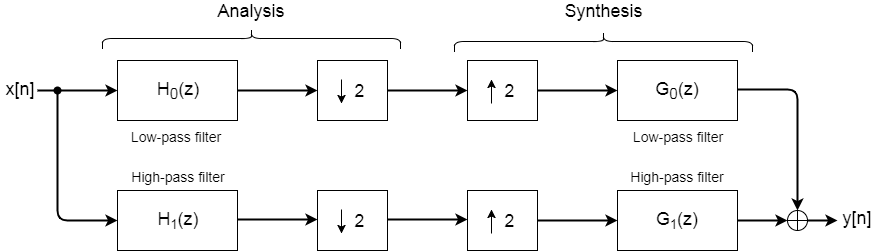
\includegraphics[width=160mm]{images/2_channel_filter_bank}
	\caption{Two-channel filter bank}
	\label{fig:2_channel_filter_bank}
\end{figure}



The idea is to determine $H_0$, $H_1$, $G_0$ and $G_1$ such that, $Y[n]$ is just a delayed version of input signal $X[n]$. This is called as perfect reconstruction filter bank. A perfect reconstruction filter bank is also known as ``biorthogonal`` and the associated filters as biorthogonal filters. 

After passing the input signal from the channel 1, it will produce:

\begin{equation} \label{eqn_wavelet_transform}
{Y_{0}(z) = \frac{1}{2}G_{0}(z)[H_{0}(z)X(z) + H_{0}(-z)X(-z)]}
\end{equation}

Similarly, for the 2nd channel, it will produce:


\begin{equation} \label{eqn_wavelet_transform}
{Y_{1}(z) = \frac{1}{2}G_{1}(z)[H_{1}(z)X(z) + H_{1}(-z)X(-z)]}
\end{equation}

Adding the output of these 2 channels will produce the final output.



\begin{equation} \label{eq1}
\begin{split}
Y(z)  &= Y_{0}(z) + Y_{1}(z) \\
&= \frac{1}{2}G_{0}(z)[H_{0}(z)X(z) + H_{0}(-z)X(-z)] + \frac{1}{2}G_{1}(z)[H_{1}(z)X(z) + H_{1}(-z)X(-z)]
\end{split}
\end{equation}


Arranging $Y(z)$ in such a way so that, one part should depends on $X(z)$ and the other part on $X(-z)$. We get,

\begin{equation} \label{eqn_wavelet_transform}
{Y(z) = \frac{1}{2}[G_{0}(z)H_{0}(z) + G_{1}(z)H_{1}(z)]X(z) + \frac{1}{2}[G_{0}(z)H_{0}(-z) + G_{1}(z)H_{1}(-z)]X(-z)}
\end{equation}

The important thing to note here is that $X(-z)$ is the aliasing part, and $X(z)$ is the distortion part.

%In order to satisfy the condition, $Y(n) = X(n-k)$ ($Y(z) = X(z)z^{-k}$) i.e., %the output signal $Y(z)$ to be some sort of delayed version of input signal, we %need to satisfy 2 conditions:

\subsection{Design of Biorthogonal Spline Wavelet Filter}

The perfect reconstruction for filter bank can be achieved if the following two conditions are satisfied.

\begin{enumerate}
	\item No aliasing: 
	\begin{equation} 
	{G_{0}(z)H_{0}(-z) + G_{1}(z)H_{1}(-z)]X(-z) = 0}
	\end{equation}
	\item No distortion:
	\begin{equation} 
	{G_{0}(z)H_{0}(z) + G_{1}(z)H_{1}(z) = mz^{-k}}
	\end{equation}
\end{enumerate}


where $m$ is constant and $k$ is a time delay.

In order to satisfy condition 1 i.e., to get rid of aliasing, one can do:

\begin{align}
	\label{eqn:antialiasing_cdn}
	\begin{split}
		G_0(z) &=  H_1(-z), \\ 
		G_1(z) &=  -H_0(-z)
	\end{split}
\end{align}


So now, we only need to find two filters values instead of four. Lets assume that,

\begin{equation}\label{eqn:p0} 
{P_0(z)=G_{0}(z)H_{0}(z)}
\end{equation}

From equation \ref{eqn:antialiasing_cdn} and \ref{eqn:p0}, we can deduce:

\begin{equation} 
{G_{1}(z)H_{1}(z) = -H_{0}(-z)G_{0}(-z) = -P_0(-z)}
\end{equation}

After getting these values, the condition 2 (no distortion) can be re-written as:

\begin{equation}\label{eqn:updated_no_distortion} 
{P_0(z) - P_0(-z) =  mz^{-k}}
\end{equation}

In the above equation, only one filter value is required i.e., $P_0(z)$ (also called half-band filter). The perfect reconstruction conditions naturally imply that both analysis and the synthesis filters are biorthogonal to each other, i.e., a biorthogonal filter bank makes sure that synthesis filter bank is the inverse of analysis filter bank.


\subsection{Steps for Designing FIR Filter Bank}
The steps for designing FIR filter bank can be summarized as:

\begin{enumerate}
	\item Design a low-pass filter for $P_0(z)$ which satisfy the equation \ref{eqn:updated_no_distortion}. One option is to use Daubechies function to find the value for $P_0(z)$: \\ 
	\begin{equation}\label{eqn:updated_no_distortion} 
	{P_0(z) = (1 + z^{-1})^{2p}Q(z)}
	\end{equation} \\
	where $p$ can be any integer and $Q(z)$ be a polynomial of degree $(2p-2)$.
	\item Factorize $P_0(z)$ to get the values for $G_0(z)$ and $H_0(z)$.
	\item Find the filter coefficients for high-pass filters using the equations \ref{eqn:antialiasing_cdn}. 
\end{enumerate}


Lets assume that, $P=2$ and and $Q(z)$ be a quadratic polynomial $(a + bz^{-1} + cz^{-2})$. Substituting these values in equation \ref{eqn:updated_no_distortion} will produce a polynomial of degree $z$:

\begin{equation} 
{P_0(z) = (1 + z^{-1})^4(a + bz^{-1} + cz^{-2})}
\end{equation}

Substituting $a = c = - \frac{1}{16}, b= 4$, we get:

\begin{equation} 
{P_0(z) = \frac{(1 + z^{-1})^4(-1 + 4z^{-1} + z^{-2})}{16}}
\end{equation}

Factorizing $P_0(z)$ to get $H_0(z)$ and $G_0(z)$. Lets say we get:

\begin{equation} \label{eq1}
\begin{split}
H_0(z) & = \frac{(1 + z^{-1})^3}{4} \\
& = \frac{(1 + 3z^{-1} + 3z^{-2} + z^{-3})}{4}
\end{split}
\end{equation}


and


\begin{equation} \label{eq1}
\begin{split}
G_0(z) & = \frac{(1 + z^{-1})(-1 + 4z^{-1} + z^{-2})}{4} \\
& = \frac{(-1 + 3z^{-1} + 3z^{-2} - z^{-3})}{4}
\end{split}
\end{equation}


Then by equation \ref{eqn:updated_no_distortion}, we have:


\begin{equation} \label{eq1}
\begin{split}
H_1(z) = G_0(-z) \\
& = \frac{(-1 - 3z^{-1} + 3z^{-2} + z^{-3})}{4}
\end{split}
\end{equation}

and

\begin{equation} \label{eq1}
\begin{split}
G_1(z) = -H_0(-z) \\
& = \frac{(-1 + 3z^{-1} _ 3z^{-2} + z^{-3})}{4}
\end{split}
\end{equation}

Therefore, the filter coefficients are:

\begin{equation}
\label{eqn:filters}
\begin{aligned}
h_0(0) & =  \quad \frac{1}{4}    & \quad &\quad  h_0(1) &= \quad \frac{3}{4} \\
h_0(2) & =  \quad \frac{3}{4}    & \quad &\quad   h_0(3) &= \quad \frac{1}{4} \\[1ex]
h_1(0) & =  \quad \frac{- 1}{4}  & \quad &\quad   h_1(1) &= \quad \frac{-3}{4} \\
h_1(2) & =  \quad \frac{3}{4}    & \quad &\quad   h_1(3) &= \quad \frac{1}{4} \\[1ex]
g_0(0) & =  \quad \frac{-1}{4}   & \quad &\quad   g_0(1) &= \quad \frac{3}{4} \\
g_0(2) & =  \quad \frac{3}{4}    & \quad &\quad   g_0(3) &= \quad \frac{-1}{4} \\[1ex]
g_1(0) & =  \quad \frac{-1}{4}   & \quad &\quad   g_1(1) &= \quad \frac{3}{4} \\
g_1(2) & =  \quad \frac{-3}{4}   & \quad &\quad   g_1(3) &= \quad \frac{1}{4}
\end{aligned}
\end{equation}




\section{Mallat's Algorithm}
The binary wavelet transform or dyadic wavelet transform of a signal $f(n)$ can be calculated by using Mallat algorithm \cite{119727} as follows:

\begin{equation} 
{ s_{2^j}f(n) = \sum h_ks_{2^{j-1}}f(n - 2^{j-1}k),   }
\end{equation}

\begin{equation} 
{ w_{2^j}f(n) = \sum g_ks_{2^{j-1}}f(n - 2^{j-1}k).   }
\end{equation}

where, $s_{2^0}f(n)$ is the original signal to be processed. In our case, it is ECG signal. $w_{2^j}f(n)$ is the wavelet coefficient i.e., the dyadic wavelet transform of the signal and $s_{2^j}f(n)$ is the approximation coefficient for the scale j. $h_k$ and $g_k$ are the coefficients of a low-pass filter and high-pass filter respectively which are defined in the equation \ref{eqn:filters}. The signal is decomposed into several frequency bands at certain scale j and then the frequency bands which have noises, are set to zero. And by using the synthesis filters, the de-noised signal can be reconstructed.



%\section{Singular Point Detection of QRS Complex Based on Wavelet Transform}
\section{Using Wavelet Transform to Identify Singular Point of QRS Complex}

\subsection{Feature Extraction Using Wavelets}
Most of the time, the important information of signal resides on the irregularities and singularities of the signal and wavelets can be used to extract that information. When the filter bank and wavelets are chosen appropriately, the wavelets are able to capture the irregularities and singularities of the signal. Mathematically, the local singularity of a signal is measured using Lipschitz exponent, the inflection points of signal $f(n)$ appear as extrema at $\frac{df(t)}{dt}$ and as zero crossing points at $\frac{d^2f(t)}{dt}$. Therefore, Mallat has suggested using a wavelet which is the first derivative of a scaling function.

\subsection{Lipschitz Exponent}
The functions which are infinitely differentiable are described as smooth or with no singularity \cite{xing2013unifying}. If at some point, the function has noncontinuous derivative, then the point is known as the singular point. The Lipschitz exponent is a good application to measure the singularity of the point.

\subsection{Relationship between Lipschitz Exponent and Modulus Maximum}
Mallat has shown in his paper \cite{119727} that, all signals and noise in there may be completely represented by their singularities and singularities are generally referred in terms of Lipschitz exponents. If a signal is $n$ times differentiable at time $t_0$, then its nth derivative is singular and it will be described as Lipschitz $\alpha$ where $\alpha > n$. If a signal is continuously differentiable at time $t_0$, then it is non-singular and has Lipschitz exponent 1.

Signals can have negative Lipschitz exponent as well. For example, many signals have singularities with positive Lipschitz exponents whereas, noise has a negative Lipschitz exponent. Therefore, having this mind, it makes it possible to separate a signal from noise if the singularities of noise can be detected and separated.

Generally, it is known that the singularity of a signal is directly proportional to the Lipschitz exponent. Therefore, as the transform scale increases, the wavelet transform modulus maxima will also get increases (Lipschitz exponent > 0) and similarly, it will decreases when Lipschitz exponent < 0. It can be seen that R wave in the original ECG signal appears as a pair of positive and negative extreme in the waveform which resulted after the decomposition of a wavelet transform.

\section{Dataset}

The MIT-BIH Arrhythmia dataset is used for the implementation of the system. It contains 48 hours of recording of 47 subjects. Each record contains 2 signals, namely MLII and V5, with a recording of 30 minutes duration. The sample rate for the recording is 360 samples per second per channel with 11-bit resolution over a 10mV range. Each record consists of 3 files:

\begin{itemize}
	\item Header file (.hea): It contains information such as the number of samples, sampling frequency, ECG signal format, number of ECG leads and their types, patient`s history and the detailed clinical information.
	
	\item ECG signals (.dat): It contains the original signal values of both MLII and V5 leads. The signals from MLII lead are considered only for the analysis.
	
	\item Attribute file (.atr): It contains the annotation information of the ECG signal, annotated by the doctors.
\end{itemize}

There is a specific python package \textit{wfdb-python} available for reading the data from the MIT-BIH dataset. The ECG signals of one of the patients can be seen in Figure \ref{fig:all_signals}. It contains 2 signals, namely, MLII and V5.


\begin{figure}[h]
	\centering
	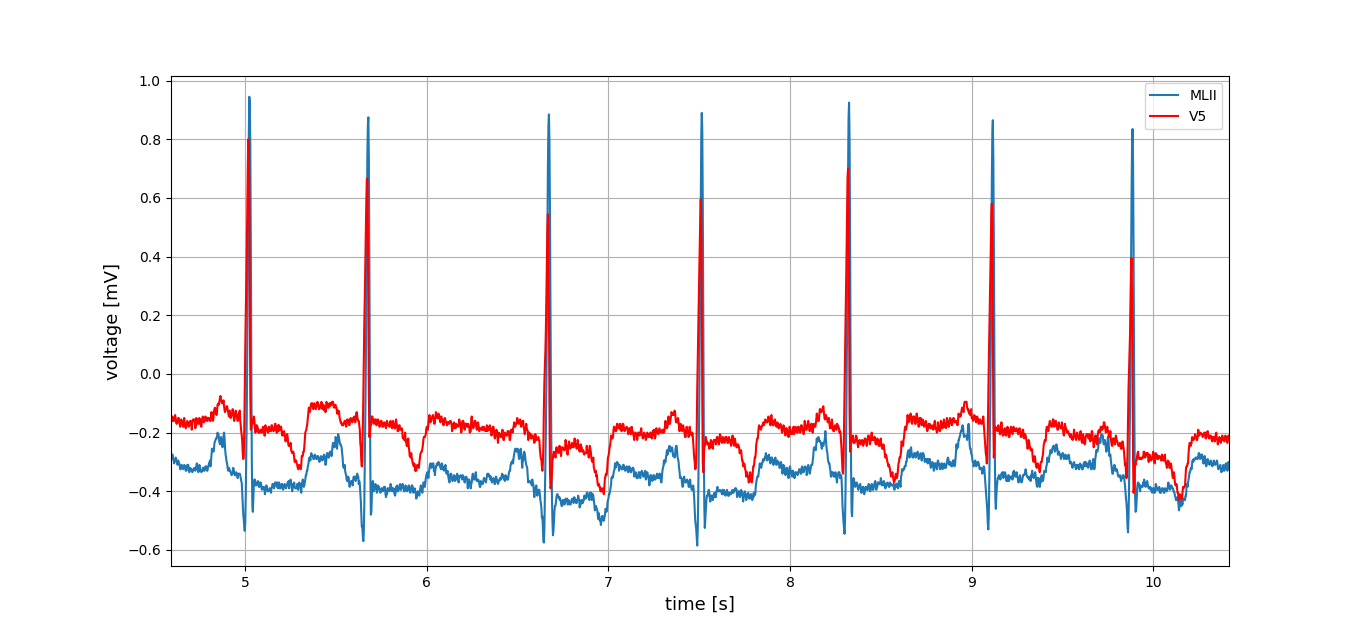
\includegraphics[width=15cm,height=12cm,keepaspectratio=true]{images/all_signals}
	\caption{
		The ECG signals from MIT-BIH dataset.
	}
	\label{fig:all_signals}
\end{figure}


The signals are in a raw form and need to be processed before they can be used. Most of the time, the signals are also contaminated with noise, baseline drift, etc. and they are required to be cleaned to get the correct values. 


\section{Preprocessing}
The ECG signal is required to be processed before it is analyzed, as it contains several noises and artifacts. The most common noises are the baseline wander and 60Hz power interference. Baseline wander generally appears because of the subject respiration or the body movements. It has a frequency range of 0Hz to 0.5Hz. The power interference affects the signals because of the electrical appliances in the surrounding.

Two different methods have been used to remove the noise and artifacts from the signal in the system implementation.

\begin{enumerate}
	\item Wavelet Transform Method
	\item Band-pass Filter Method
\end{enumerate}

\begin{figure}[h]
	\centering
	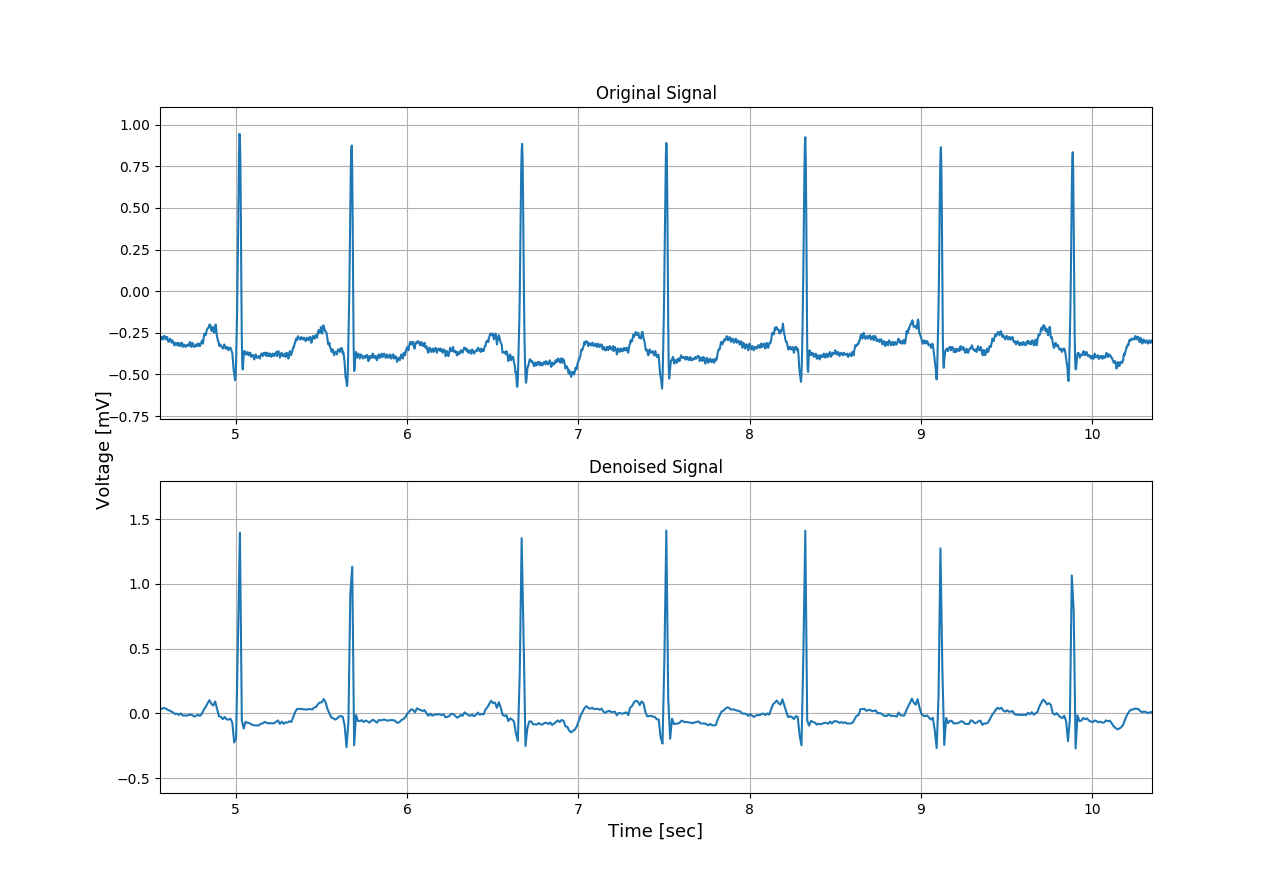
\includegraphics[width=15cm,height=12cm,keepaspectratio=true]{images/wavelet_denoised_1}
	\caption{
		The filtered ECG signal using wavelet.
	}
	\label{fig:wavelet_denoised}
\end{figure}


\subsection{Wavelet Transform Method}

The wavelet transform is a very interesting technique for analyzing the signal in the time-frequency domain. It distributes the signal in such a way that the resulting block is well localized in both time and frequency. Decomposition of the signal into different frequency bands is obtained by passing the signal through high-pass and low-pass filter respectively, which results in 2 sets of coefficients namely, approximation coefficients and detail coefficients. The approximation coefficients contain the low-pass filter output and the detail coefficients contain the high-pass filter output. The next step split the approximation coefficients again into 2 parts using the same process and so on.

The original signal contains the high-frequency noise and the baseline drift. The wavelet transform can be used to remove the corresponding noises and the baseline drift. The process starts by decomposing the original signal into 8 layers using wavelet type bior2.6, which results in the corresponding detail and approximation coefficients. Mostly, the layers 1 and 2 of the detail coefficients contain the high-frequency noise and the layer 8 of the approximation coefficients contain the baseline drift. Therefore, the layers 1 and 2 of the detail coefficients and layer 8 of the approximation coefficients are set to 0; which then results in the de-noised signal with no baseline drift. The resulting ECG signal can be seen in the Figure \ref{fig:wavelet_denoised}. 




\subsection{Band-pass Filter Method}
A band-pass filter is a type of filter which passes frequencies only in a certain range or spread without disturbing the input signal. The range of frequencies, let say, f1 and f2, are called the frequency passband.

A band-pass filter can be used to reduce the baseline drift, motion artifacts and high-frequency noise from the ECG signal. A passband of 3 Hz to 45 Hz has been used. After passing the ECG signal through the band-pass filter, the resulting signal produced is the de-noised signal with no high-frequency and baseline drift. The de-noised signal can be seen in the Figure \ref{fig:bandpass_denoised}. 

\begin{figure}[h]
	\centering
	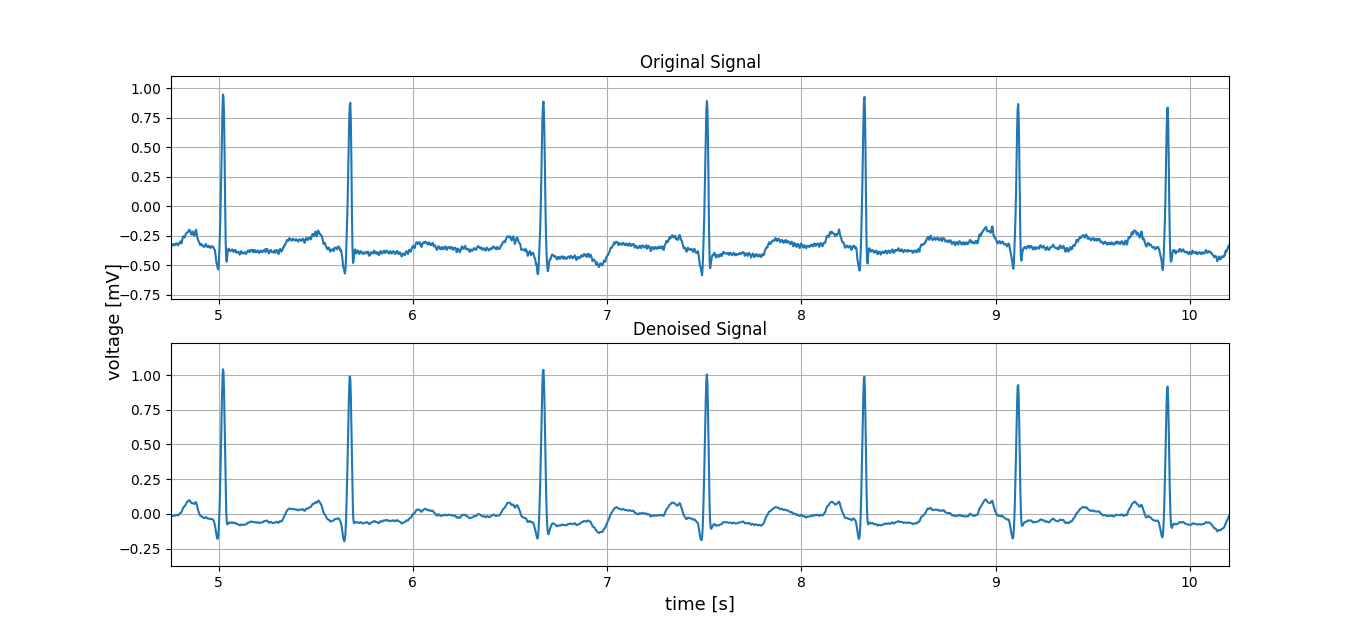
\includegraphics[width=15cm,height=12cm,keepaspectratio=true]{images/bandpass_denoised_1}
	\caption{
		The filtered ECG signal using bandpass filter.
	}
	\label{fig:bandpass_denoised}
\end{figure}


\renewcommand{\arraystretch}{2}
\begin{table}
	\caption{Wavelet transform ECG signal frequency range\cite{shang2014qrs}.} \label{tab:qrsenergy}
	
	\begin{center}
		\begin{tabular}{ | l | r | }
			\hline
			Transform Scale & Frequency Range (Hz) \\ \hline
			${2^1}$  & 90.0{\raise.17ex\hbox{$\scriptstyle\sim$}}180.0 \\ \hline
			${2^2}$  & 29.92{\raise.17ex\hbox{$\scriptstyle\sim$}}84.24  \\ \hline
			${2^3}$  & 1.52{\raise.17ex\hbox{$\scriptstyle\sim$}}38.88  \\ \hline
			${2^4}$  & 5.76{\raise.17ex\hbox{$\scriptstyle\sim$}}19.44  \\ 
			\hline
		\end{tabular}
	\end{center}
	
\end{table}


\section{QRS Detection}\label{sec:ecg_det}
QRS detection is the basis for processing the ECG signal. Regardless of what application is required, the accurate detection of QRS is a pre-requisite for feature extraction. A good wavelet base can help detect the features of ECG signal more appropriately with speed and accuracy. Therefore, Biorthogonal spline wavelet is used to detect QRS wave. Biorthogonal spline wavelet transform of ECG signal is calculated using the Mallat algorithm. Figure ~\ref{fig:detail_coefficients} shows the Biorthogonal spline wavelet transform of ECG signal at 4 different scales.

\begin{figure}[htpb]
	\centering
	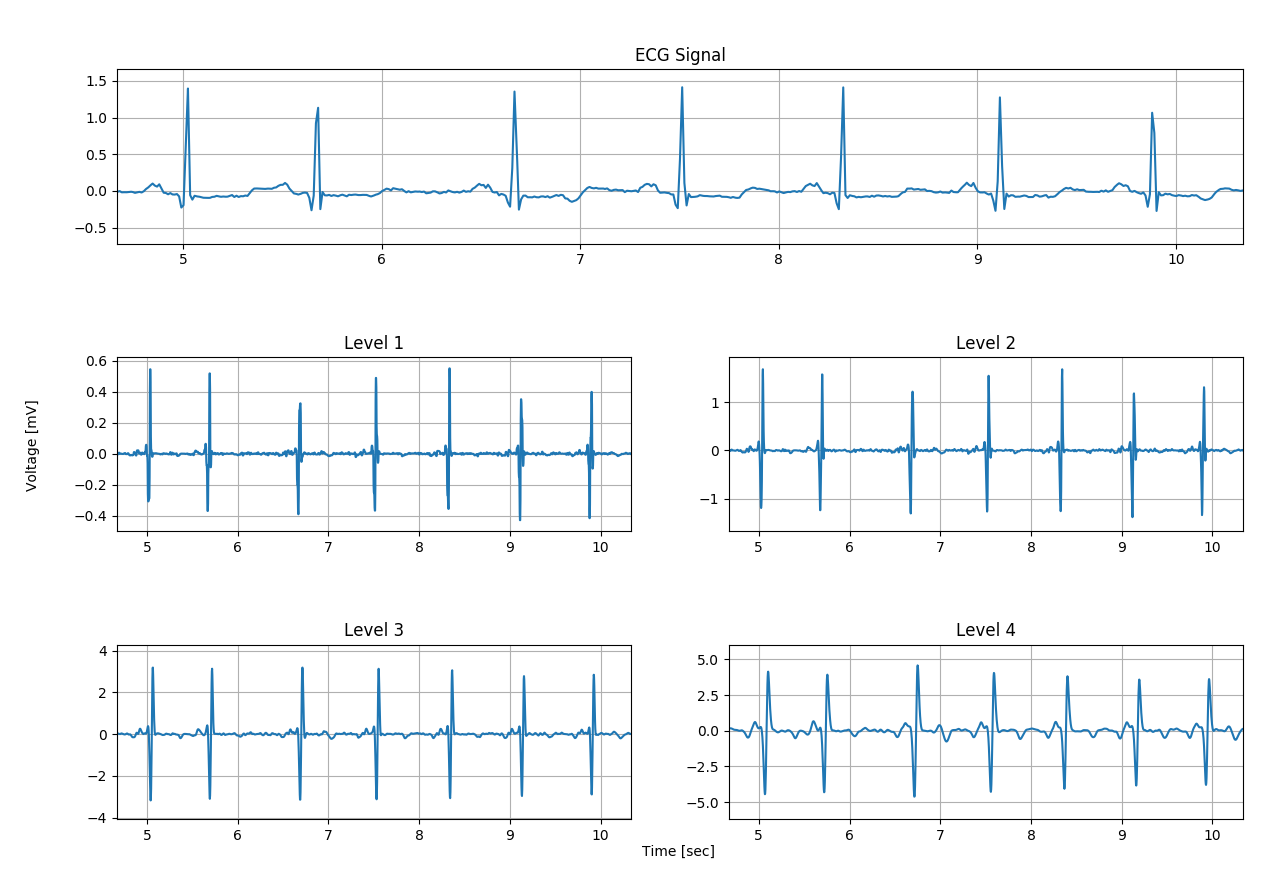
\includegraphics[width=17cm,height=17cm,keepaspectratio=true]{images/detail_coefficients}
	\caption{
		ECG signal and its decomposition at different scales.
	}
	\label{fig:detail_coefficients}
\end{figure}

Most of the QRS complex energy lies in the 3rd scale as can be seen in Table \ref{tab:qrsenergy}, therefore, the maximal minimal method can be used on the 3rd layer of the detail coefficient to find the R waves.  The process starts by taking the first derivative of the 3rd layer to find the maximum and minimum points and then the 2nd derivative to locate the actual maximum and minimum values. The resulting waves are shown in Figure \ref{fig:maximas_on_level_3}. As it can be seen that, there are other peaks available as well, therefore, to get the maximum and minimum pair only, a threshold needs to be set. And all the values that do not fulfill the threshold should be discarded. 
For finding the threshold, the result of the 2nd derivative is divided into 4 parts and from each part, the maximum value is located. After getting the values, the average is calculated for these values and that average is then divided by 3. The resultant value is a new threshold. The pair can be seen in Figure \ref{fig:max_pair}.

\begin{figure}[htpb]
	\centering
	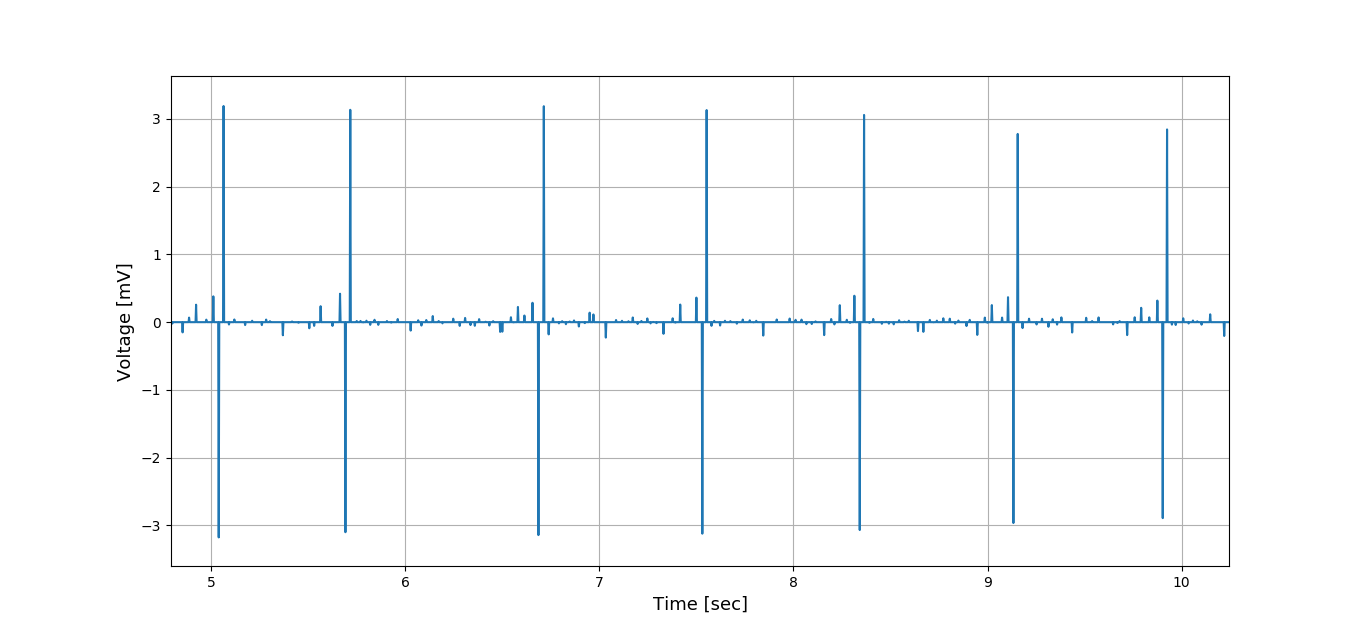
\includegraphics[width=15cm,height=15cm,keepaspectratio=true]{images/maximas_on_level_3}
	\caption{
		Maximum and minimum values on scale 3.
	}
	\label{fig:maximas_on_level_3}
\end{figure}

\begin{figure}[htpb]
	\centering
	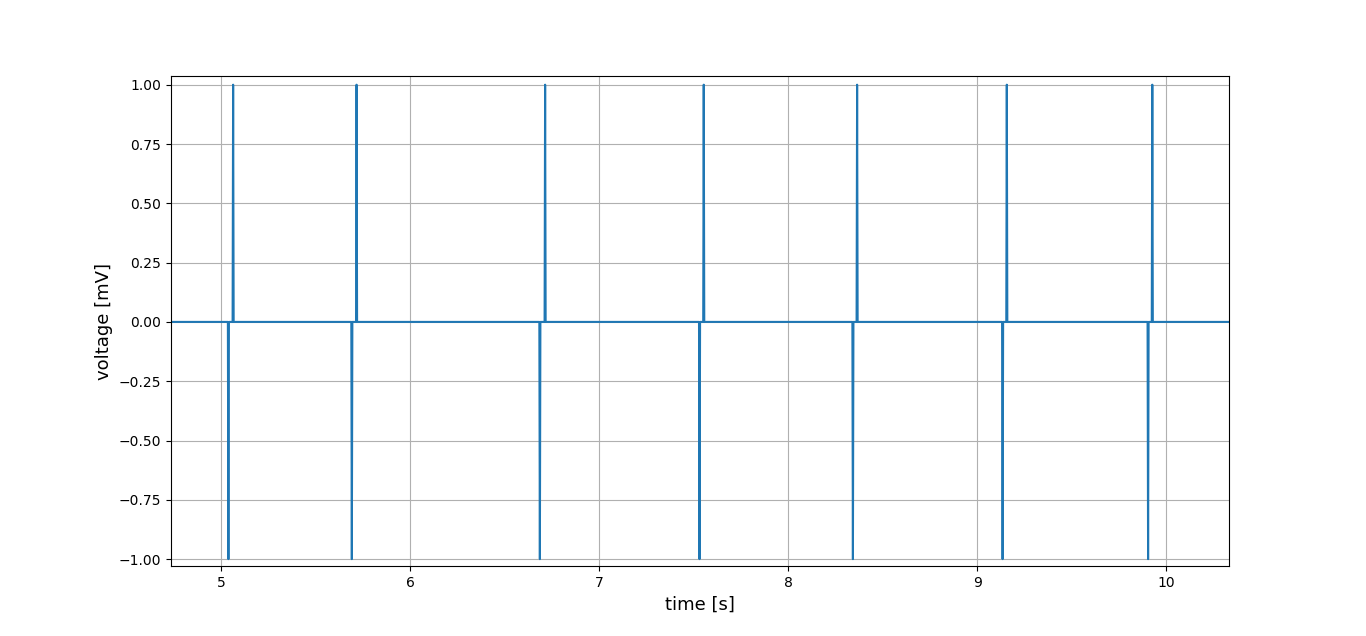
\includegraphics[width=15cm,height=12cm,keepaspectratio=true]{images/max_pair}
	\caption{
		Maximum and minimum values pair for finding the R peaks.
	}
	\label{fig:max_pair}
\end{figure}

The value of R wave lies at the zero-crossing point (with a little delay) which is between the maximum and the minimum value pair. For compensating the delay, a maximum value can be searched in the window of 20 points to the zero-crossing point. The detected R-peaks can be seen in Figure \ref{fig:r_peaks}. The flow chart for finding the R peaks is shown in Figure \ref{fig:r_peaks_flow_chart}.

\begin{figure}[htpb]
	\centering
	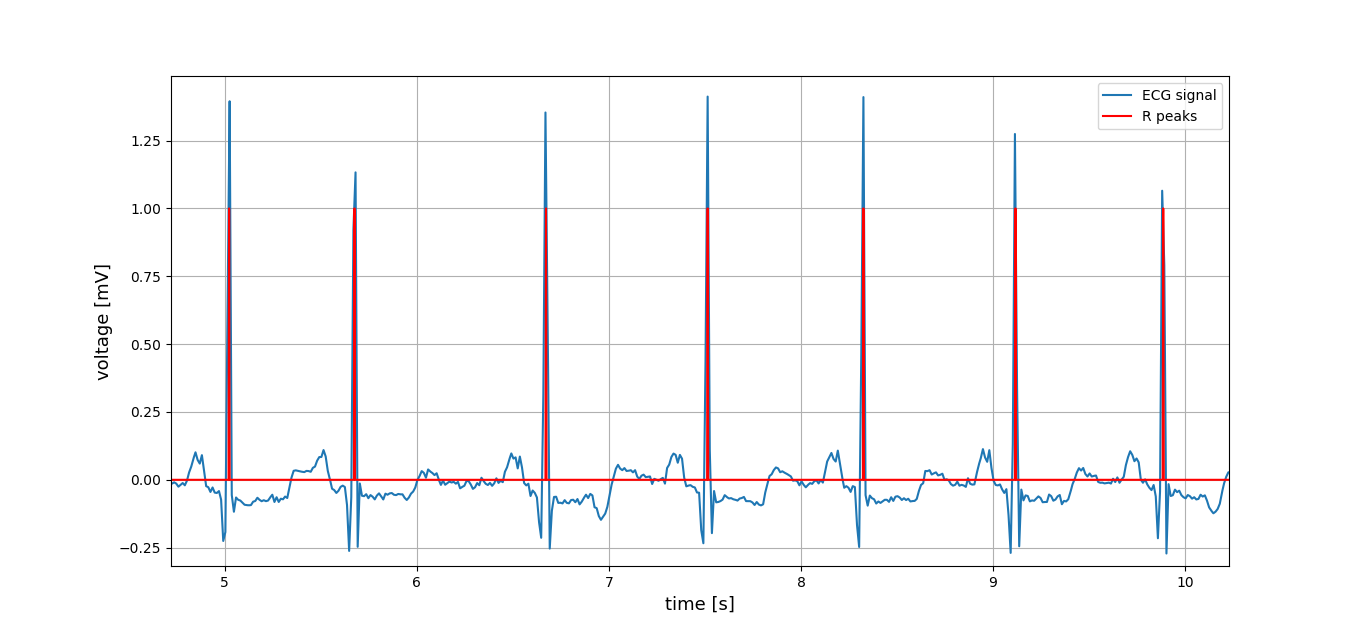
\includegraphics[width=15cm,height=15cm,keepaspectratio=true]{images/r_peaks}
	\caption{
		Detected R peaks.
	}
	\label{fig:r_peaks}
\end{figure}


\begin{figure}[htpb]
	\centering
	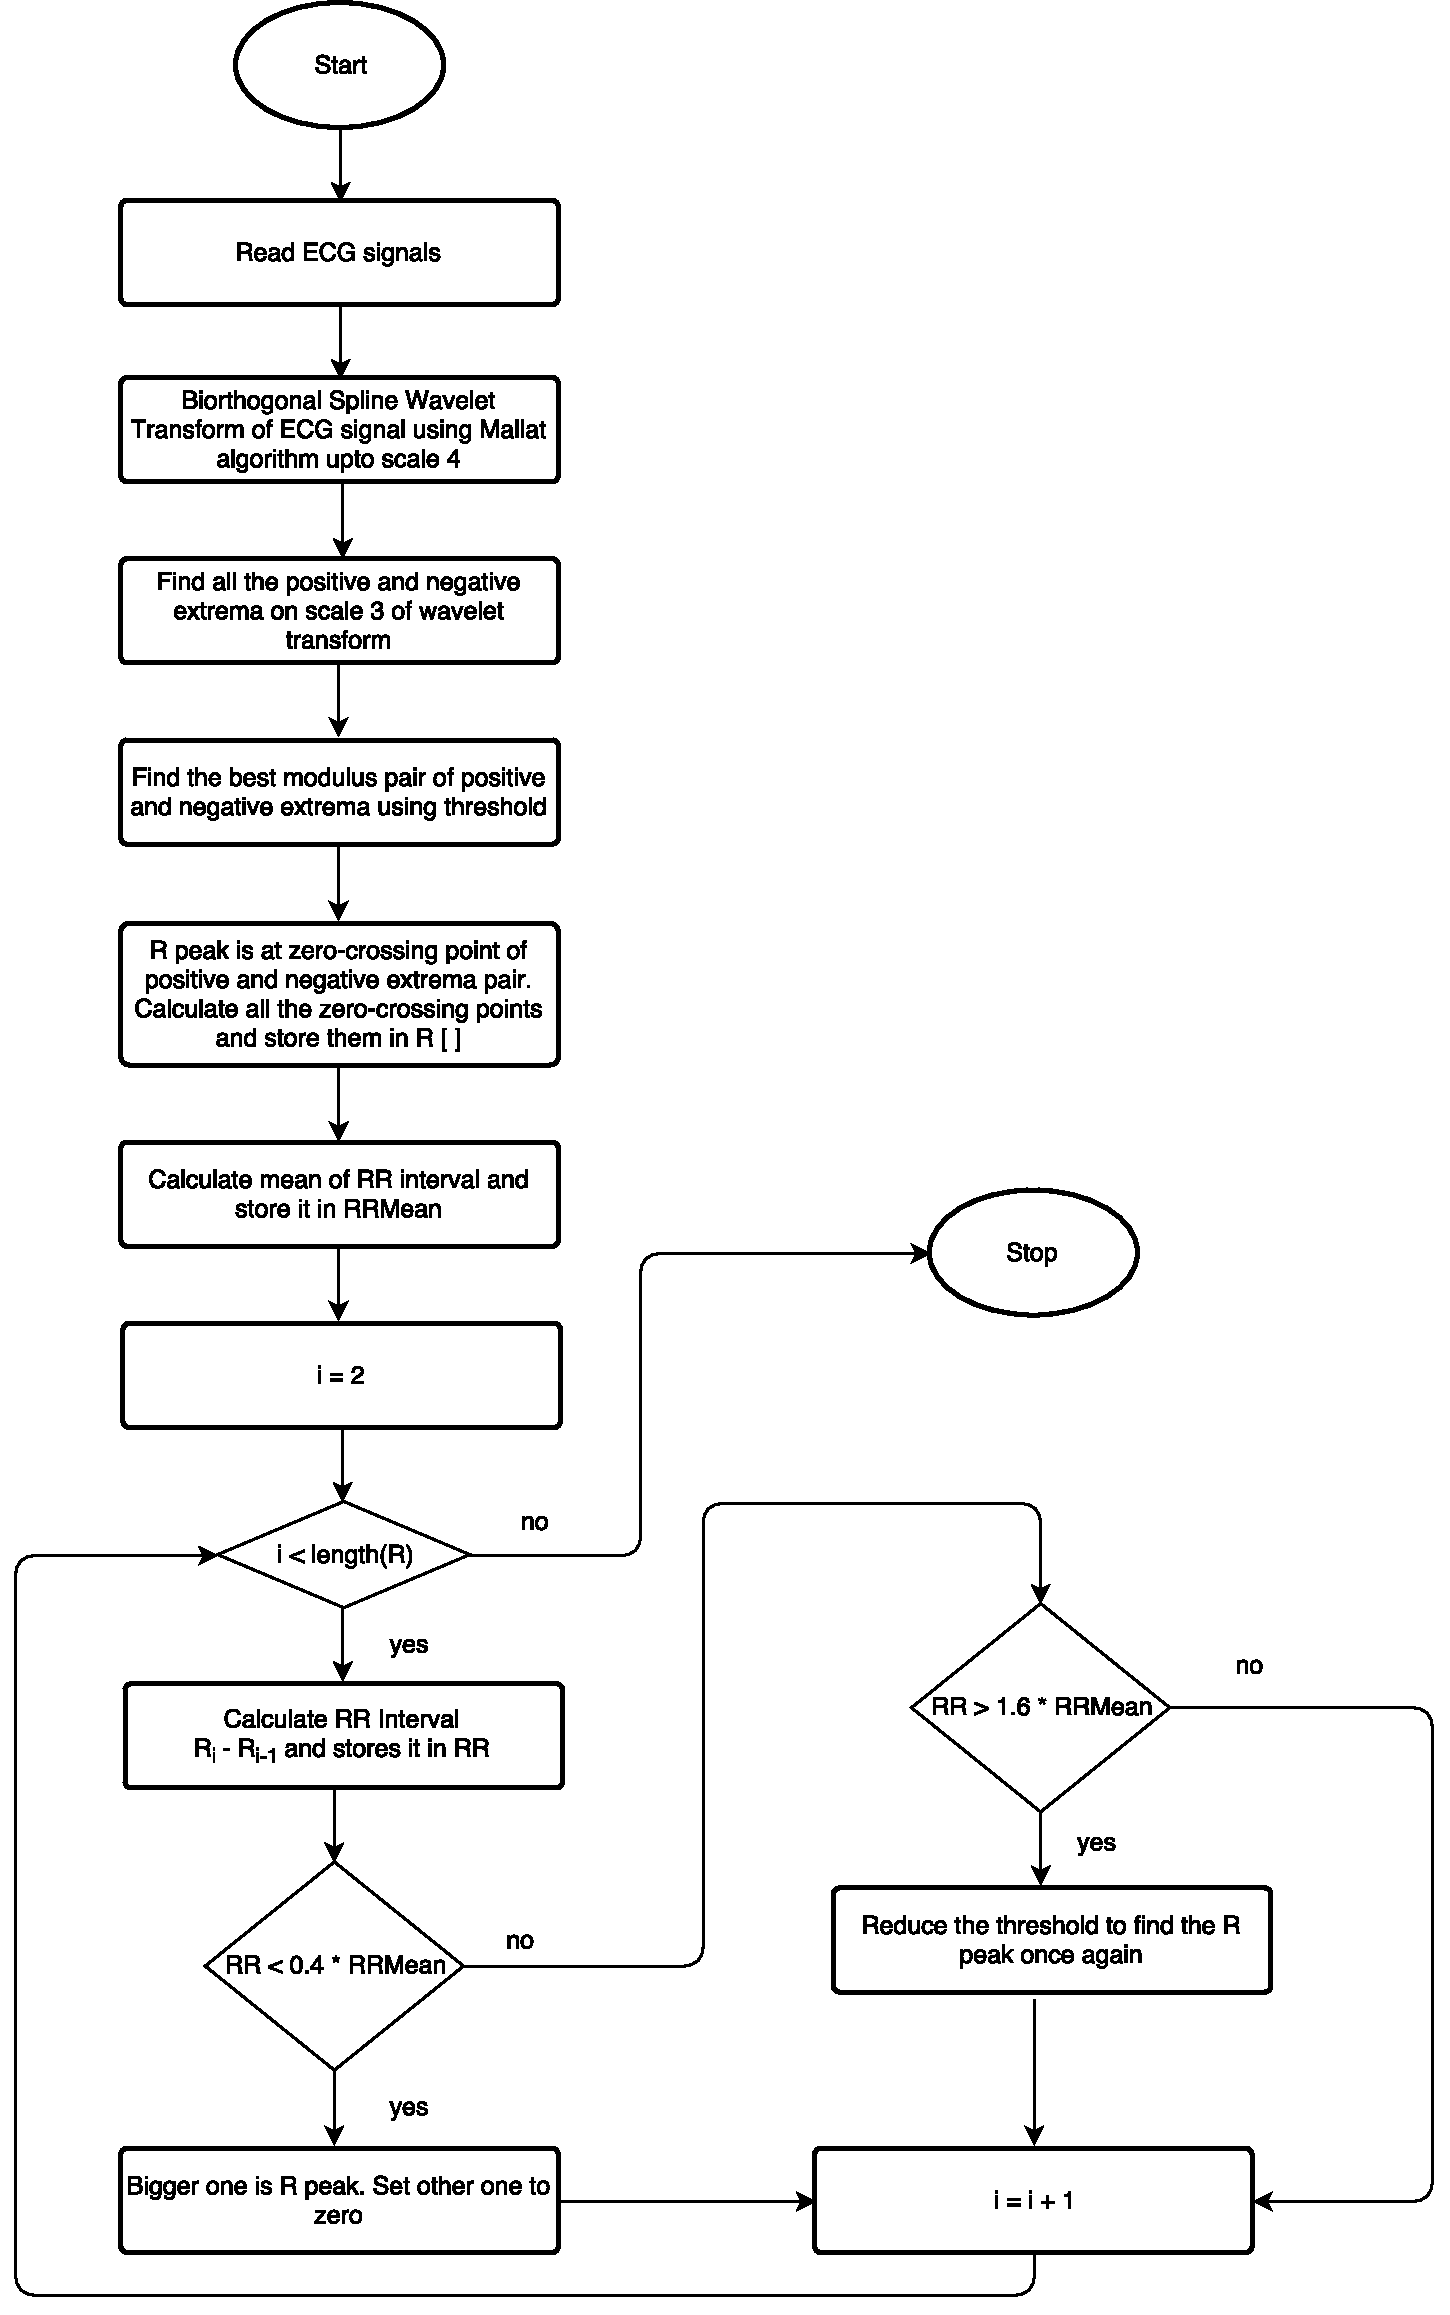
\includegraphics[width=25cm,height=22cm,keepaspectratio=true]{images/qrs.pdf}
	\caption{
		R peak flow chart.
	}
	\label{fig:r_peaks_flow_chart}
\end{figure}



After getting the R-peaks, Q and S peaks have to be detected. Q and S wave generally are of high frequency; therefore, their energies are mainly on the 1st scale. For finding the Q wave, the algorithm starts by looking on the left side of the R wave and finds the first non-zero value i.e. the Q wave. And because of the delay, the minimum value is searched in the window of 10 points to the detected Q wave. The same process is executed for the S wave, but in this case, the direction was on the right side of the R wave. The detected QRS complex can be seen in Figure \ref{fig:qrs_peaks}.

\begin{figure}[htpb]
	\centering
	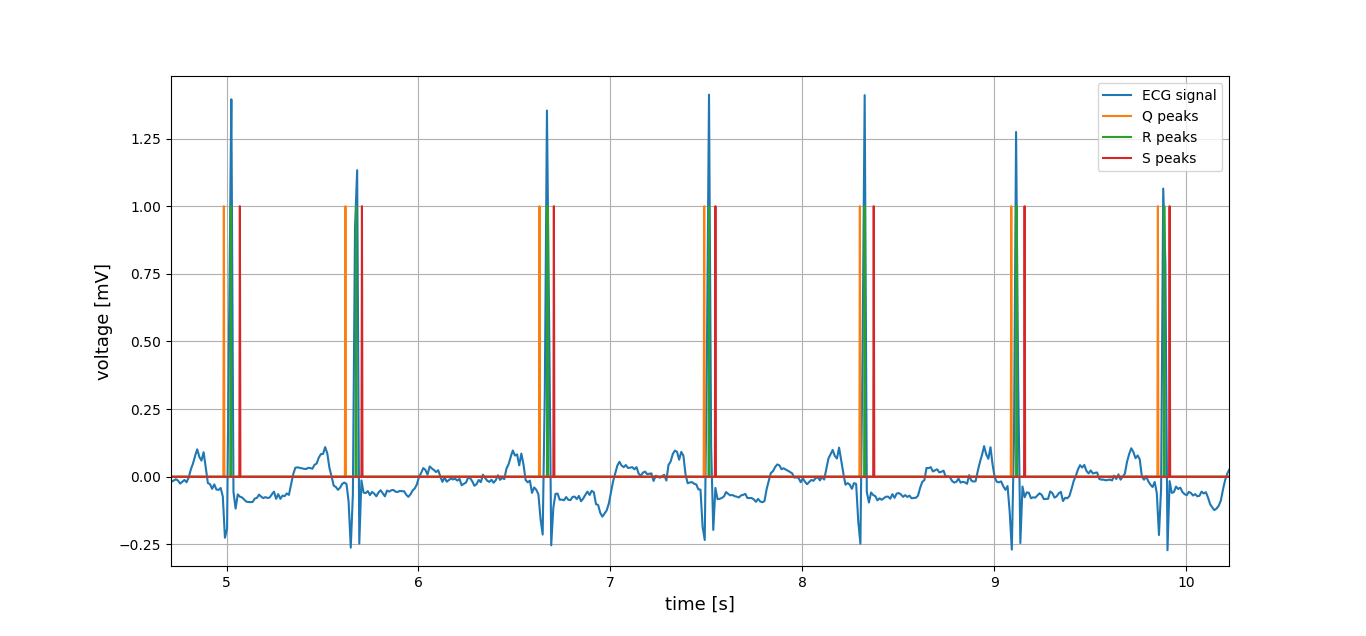
\includegraphics[width=15cm,height=15cm,keepaspectratio=true]{images/qrs}
	\caption{
		Detected Q, R and S peaks.
	}
	\label{fig:qrs_peaks}
\end{figure}


\begin{figure}[htpb]
	\centering
	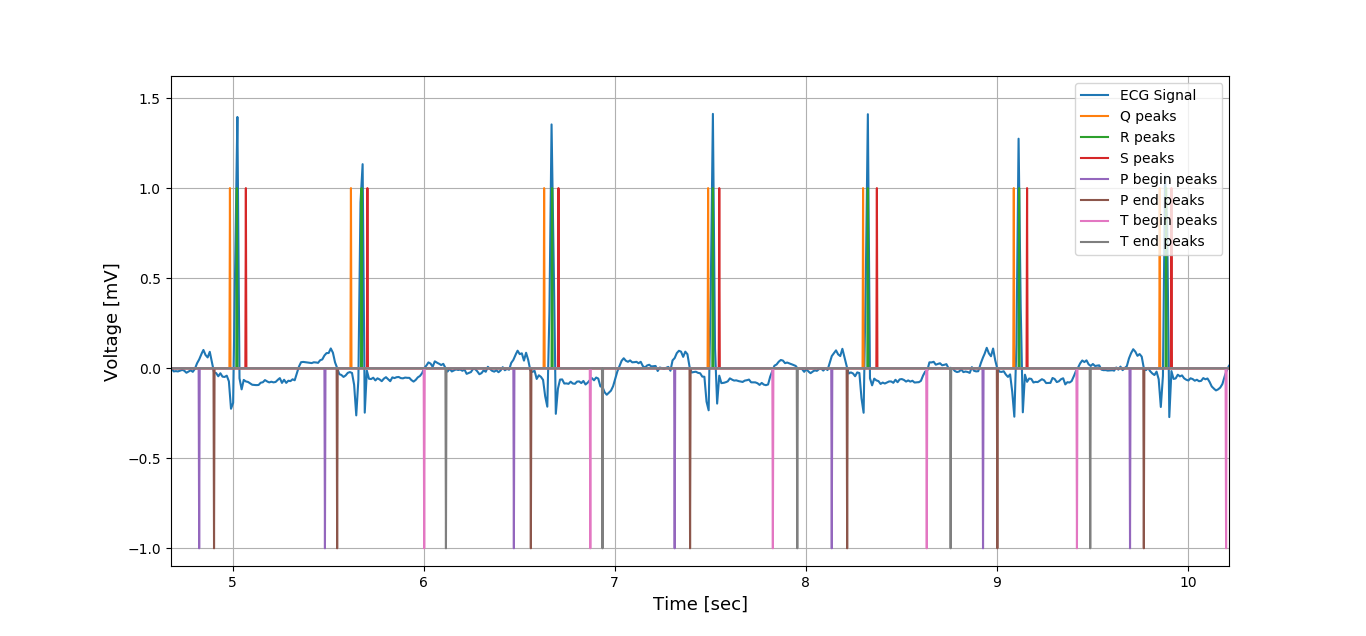
\includegraphics[width=15cm,height=15cm,keepaspectratio=true]{images/pqrst}
	\caption{
		Detected P,Q,R,S and T waves.
	}
	\label{fig:pqrst}
\end{figure}



\begin{figure}[htpb]
	\centering
	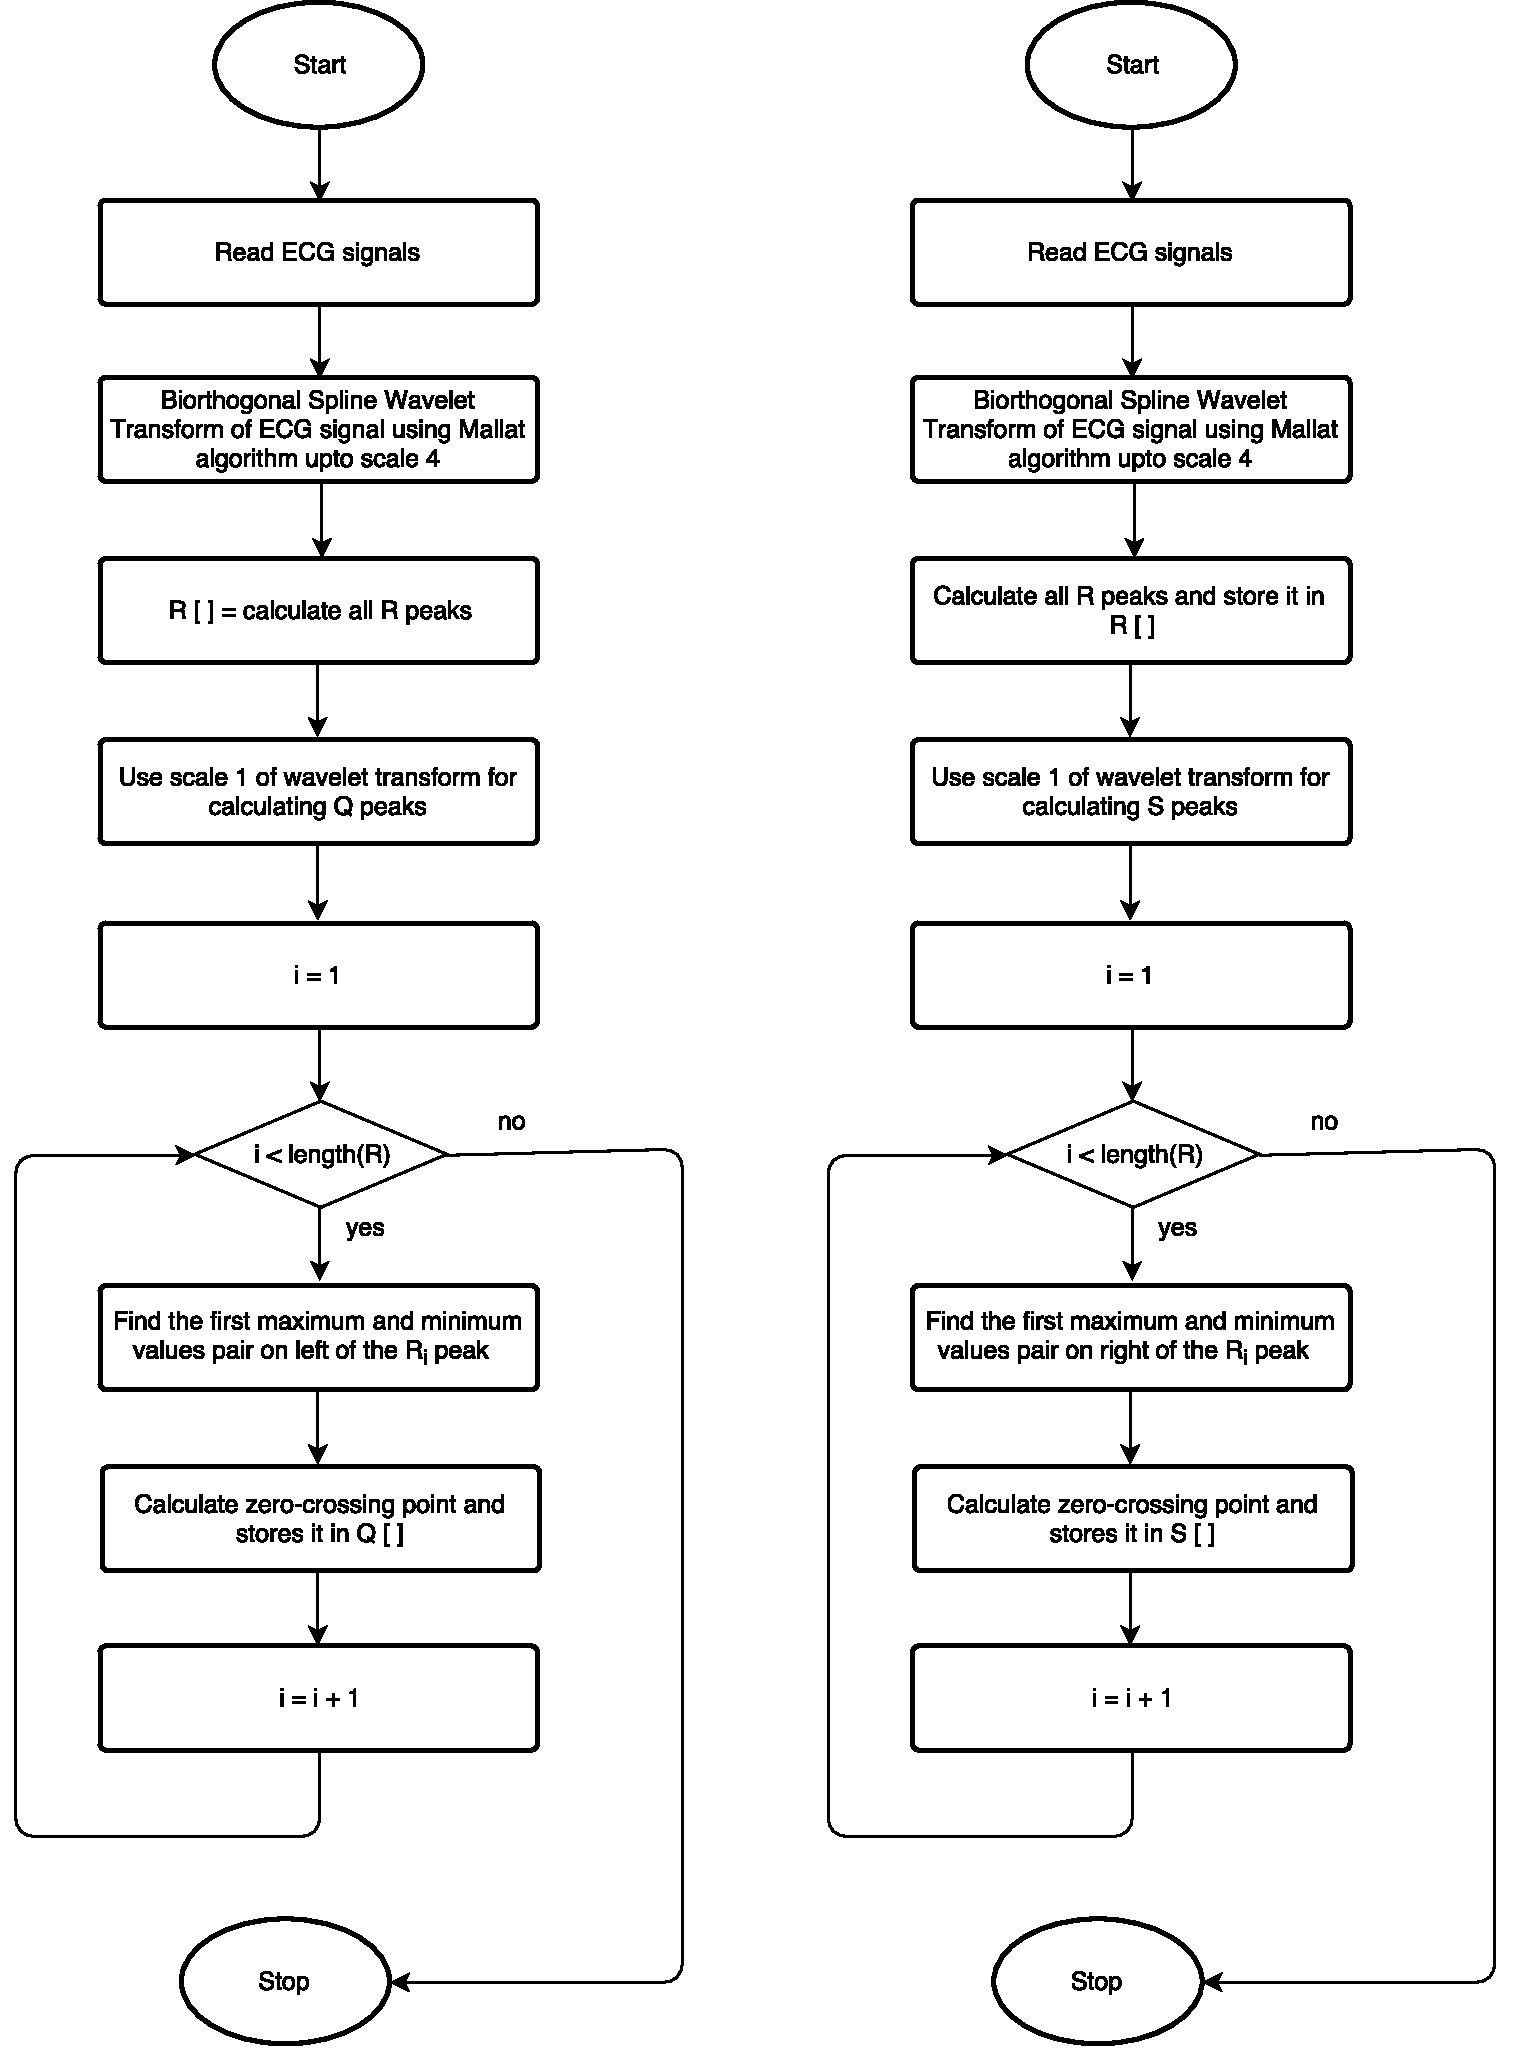
\includegraphics[width=25cm,height=22cm,keepaspectratio=true]{images/q-and-s.pdf}
	\caption{
		Q and S peak flow chart.
	}
	\label{fig:qs}
\end{figure}



After detecting the QRS complex, P and T waves are required to be detected as they also have very important significance to identify the arrhythmia. P wave generally occurred before the QRS complex and T wave after the QRS complex, therefore, they can be detected based on QRS location.

\section{P and T Wave Detection}
Most of the P and T waves energy lies on the scale 4 and the QRS complex energy lies on the scale 3 of detail coefficient. If QRS complex (that was detected on scale 3) is used, it sometimes misses the P wave or identifies the wrong position. Therefore, it is first required to detect QRS complex on scale 4 and then find P and T waves. The same algorithm is used to detect the QRS complex on scale 4 that is used to detect on scale 3, as described in section \ref{sec:ecg_det}.

After getting the QRS on scale 4, a window size of 100 is used for detecting the P wave. The starting point of the window is one sample less than from Q wave position and if the window size is added to this position, we get the beginning of the window. RR interval is also calculated between the 2 consecutive R peaks. 1/3 of the RR interval is used for detecting the P wave and 2/3 of the RR interval is used for detecting the T wave. Once the window is identified on the scale 4, the max and min values are identified in that window as P wave lies on the zero-crossing point of min and max pair. The average is taken to calculate the P wave position of scale 4. Once the P wave position is calculated, the P wave is identified relatively on the original signal. One point to note here is that the scale 4 data is shifted because of filtering, therefore, it is required to shift the detected position few samples back to get the appropriate value.

The same approach is used for detecting the T wave, but instead of looking the window before the QRS complex, here the window is searched after the QRS complex for detecting the T wave.

All detected waves can be seen in Figure \ref{fig:pqrst}. The flow chart for finding the P wave and T wave is shown in Figures \ref{fig:p_peaks_flow_chart} and \ref{fig:t_peaks_flow_chart} respectively.


\begin{figure}[htpb]
	\centering
	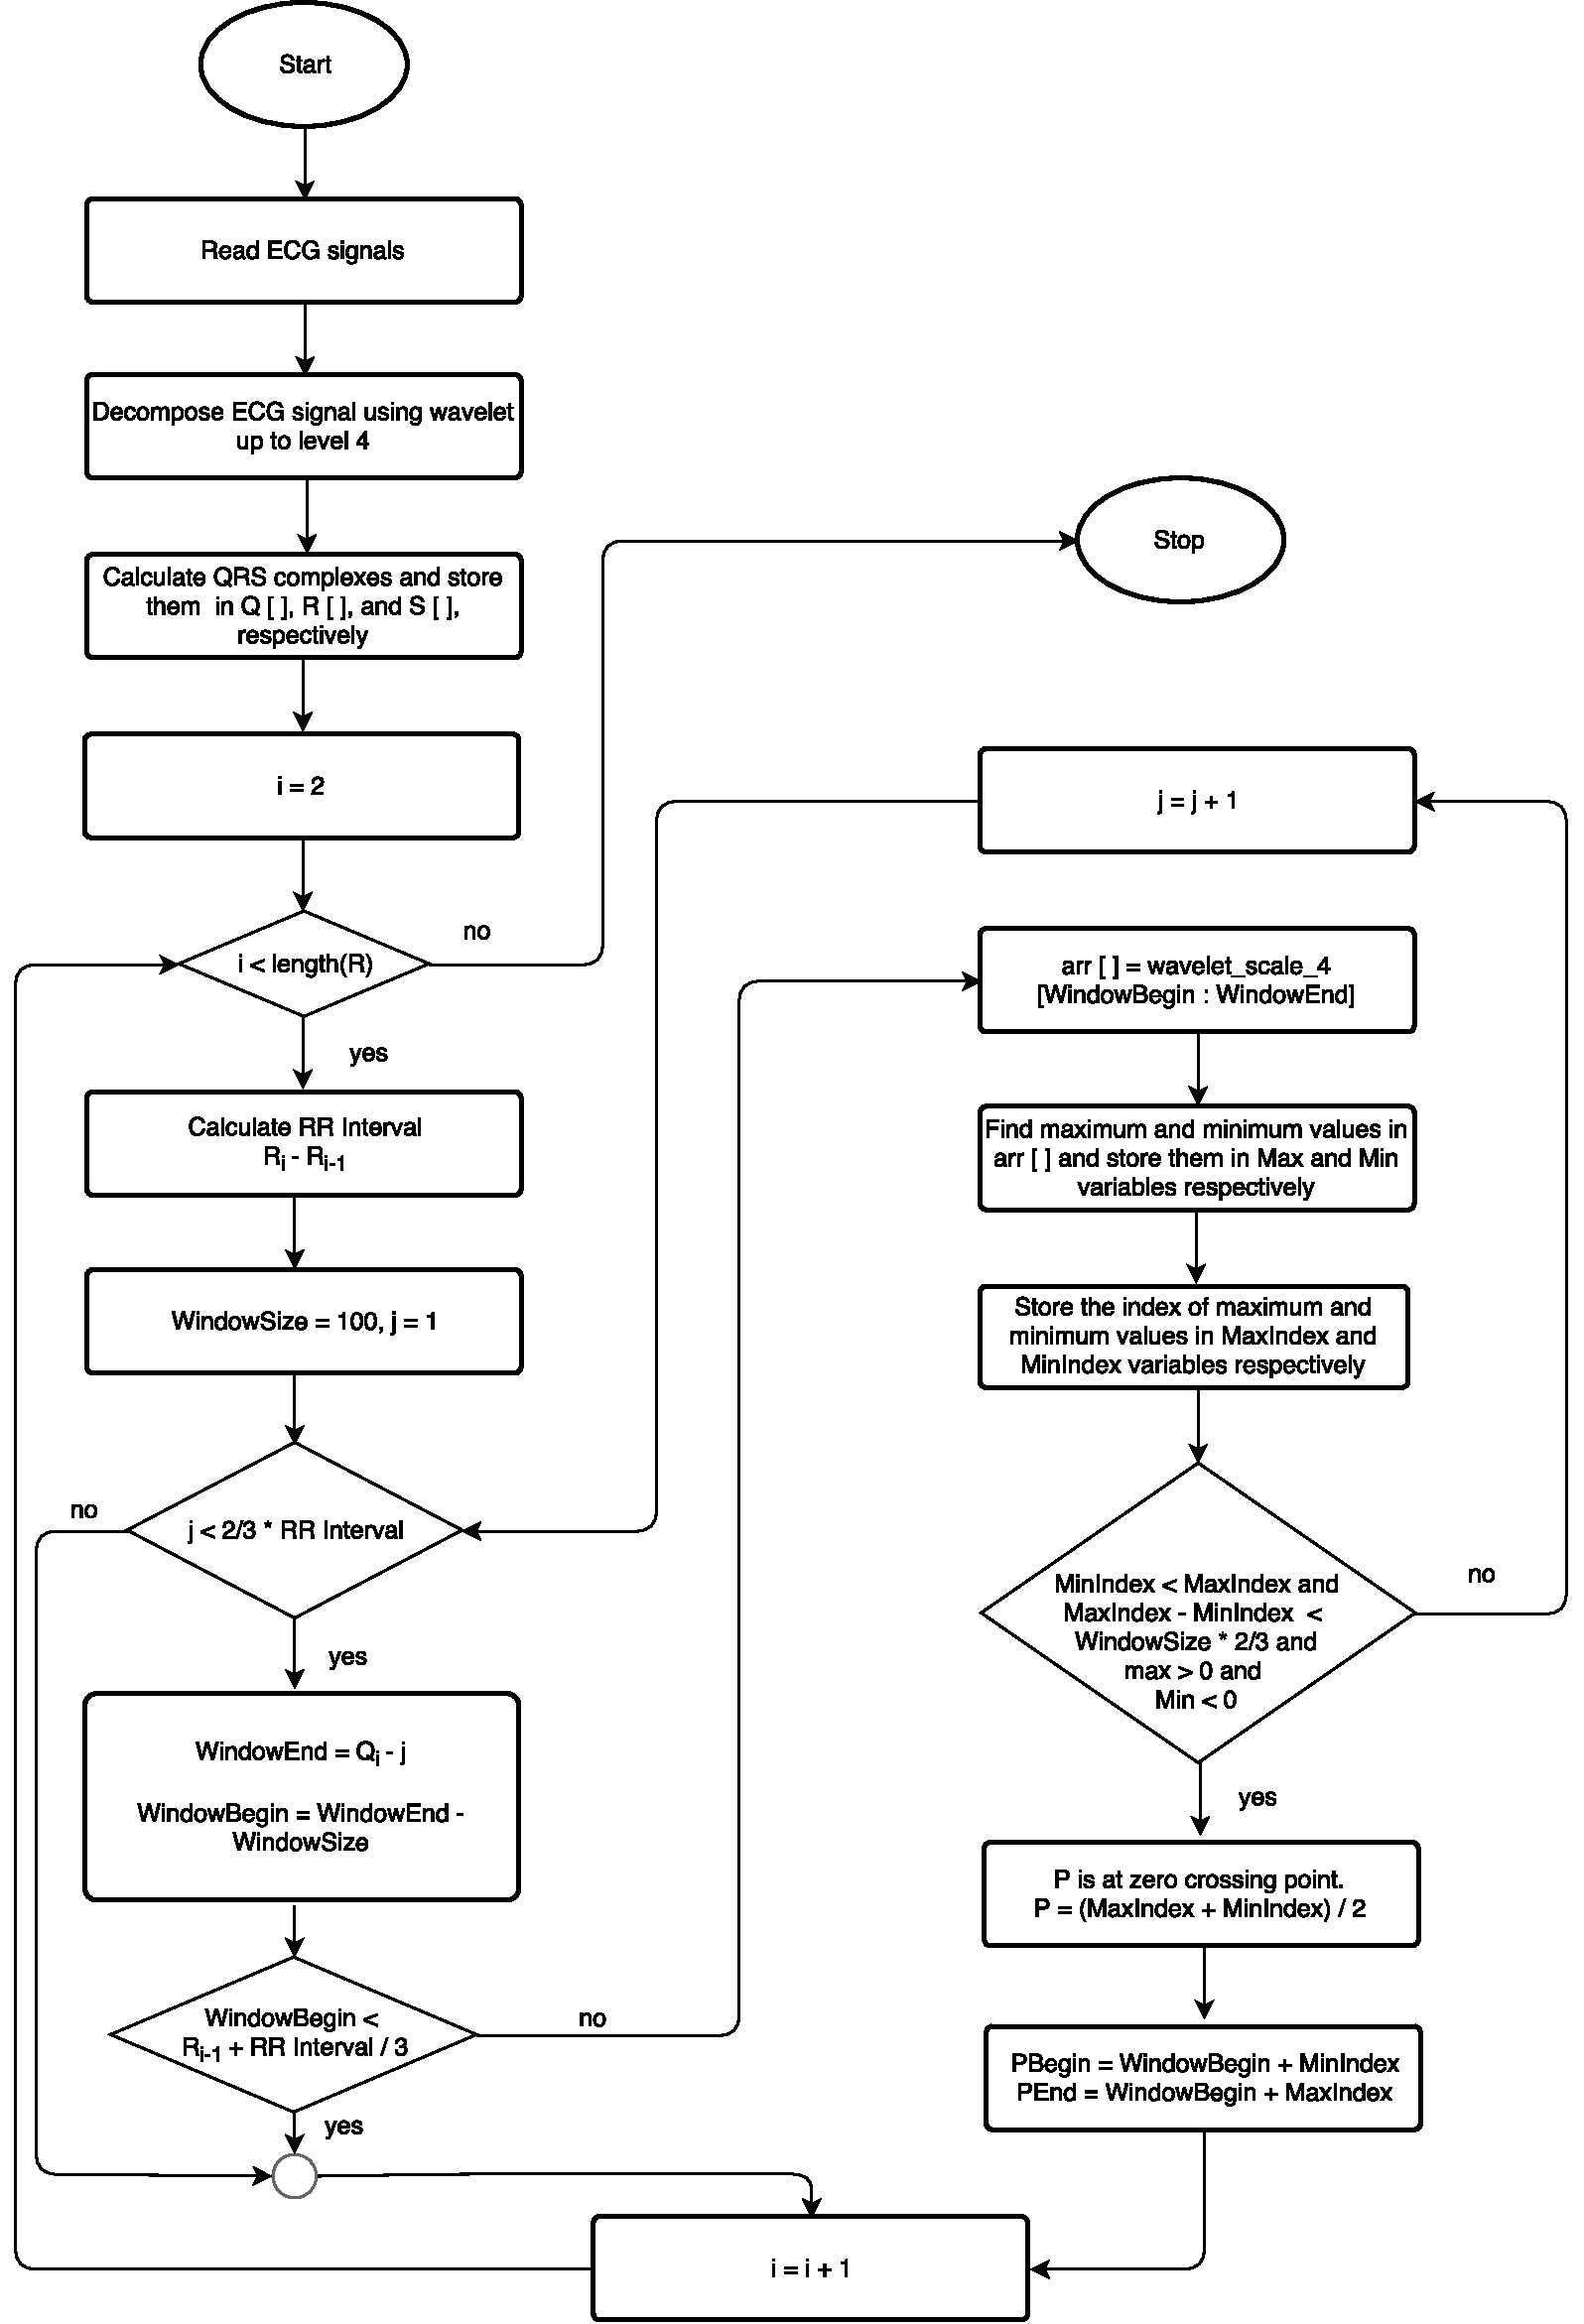
\includegraphics[width=25cm,height=22cm,keepaspectratio=true]{images/p_Wave.pdf}
	\caption{
		P wave flow chart.
	}
	\label{fig:p_peaks_flow_chart}
\end{figure}

\begin{figure}[htpb]
	\centering
	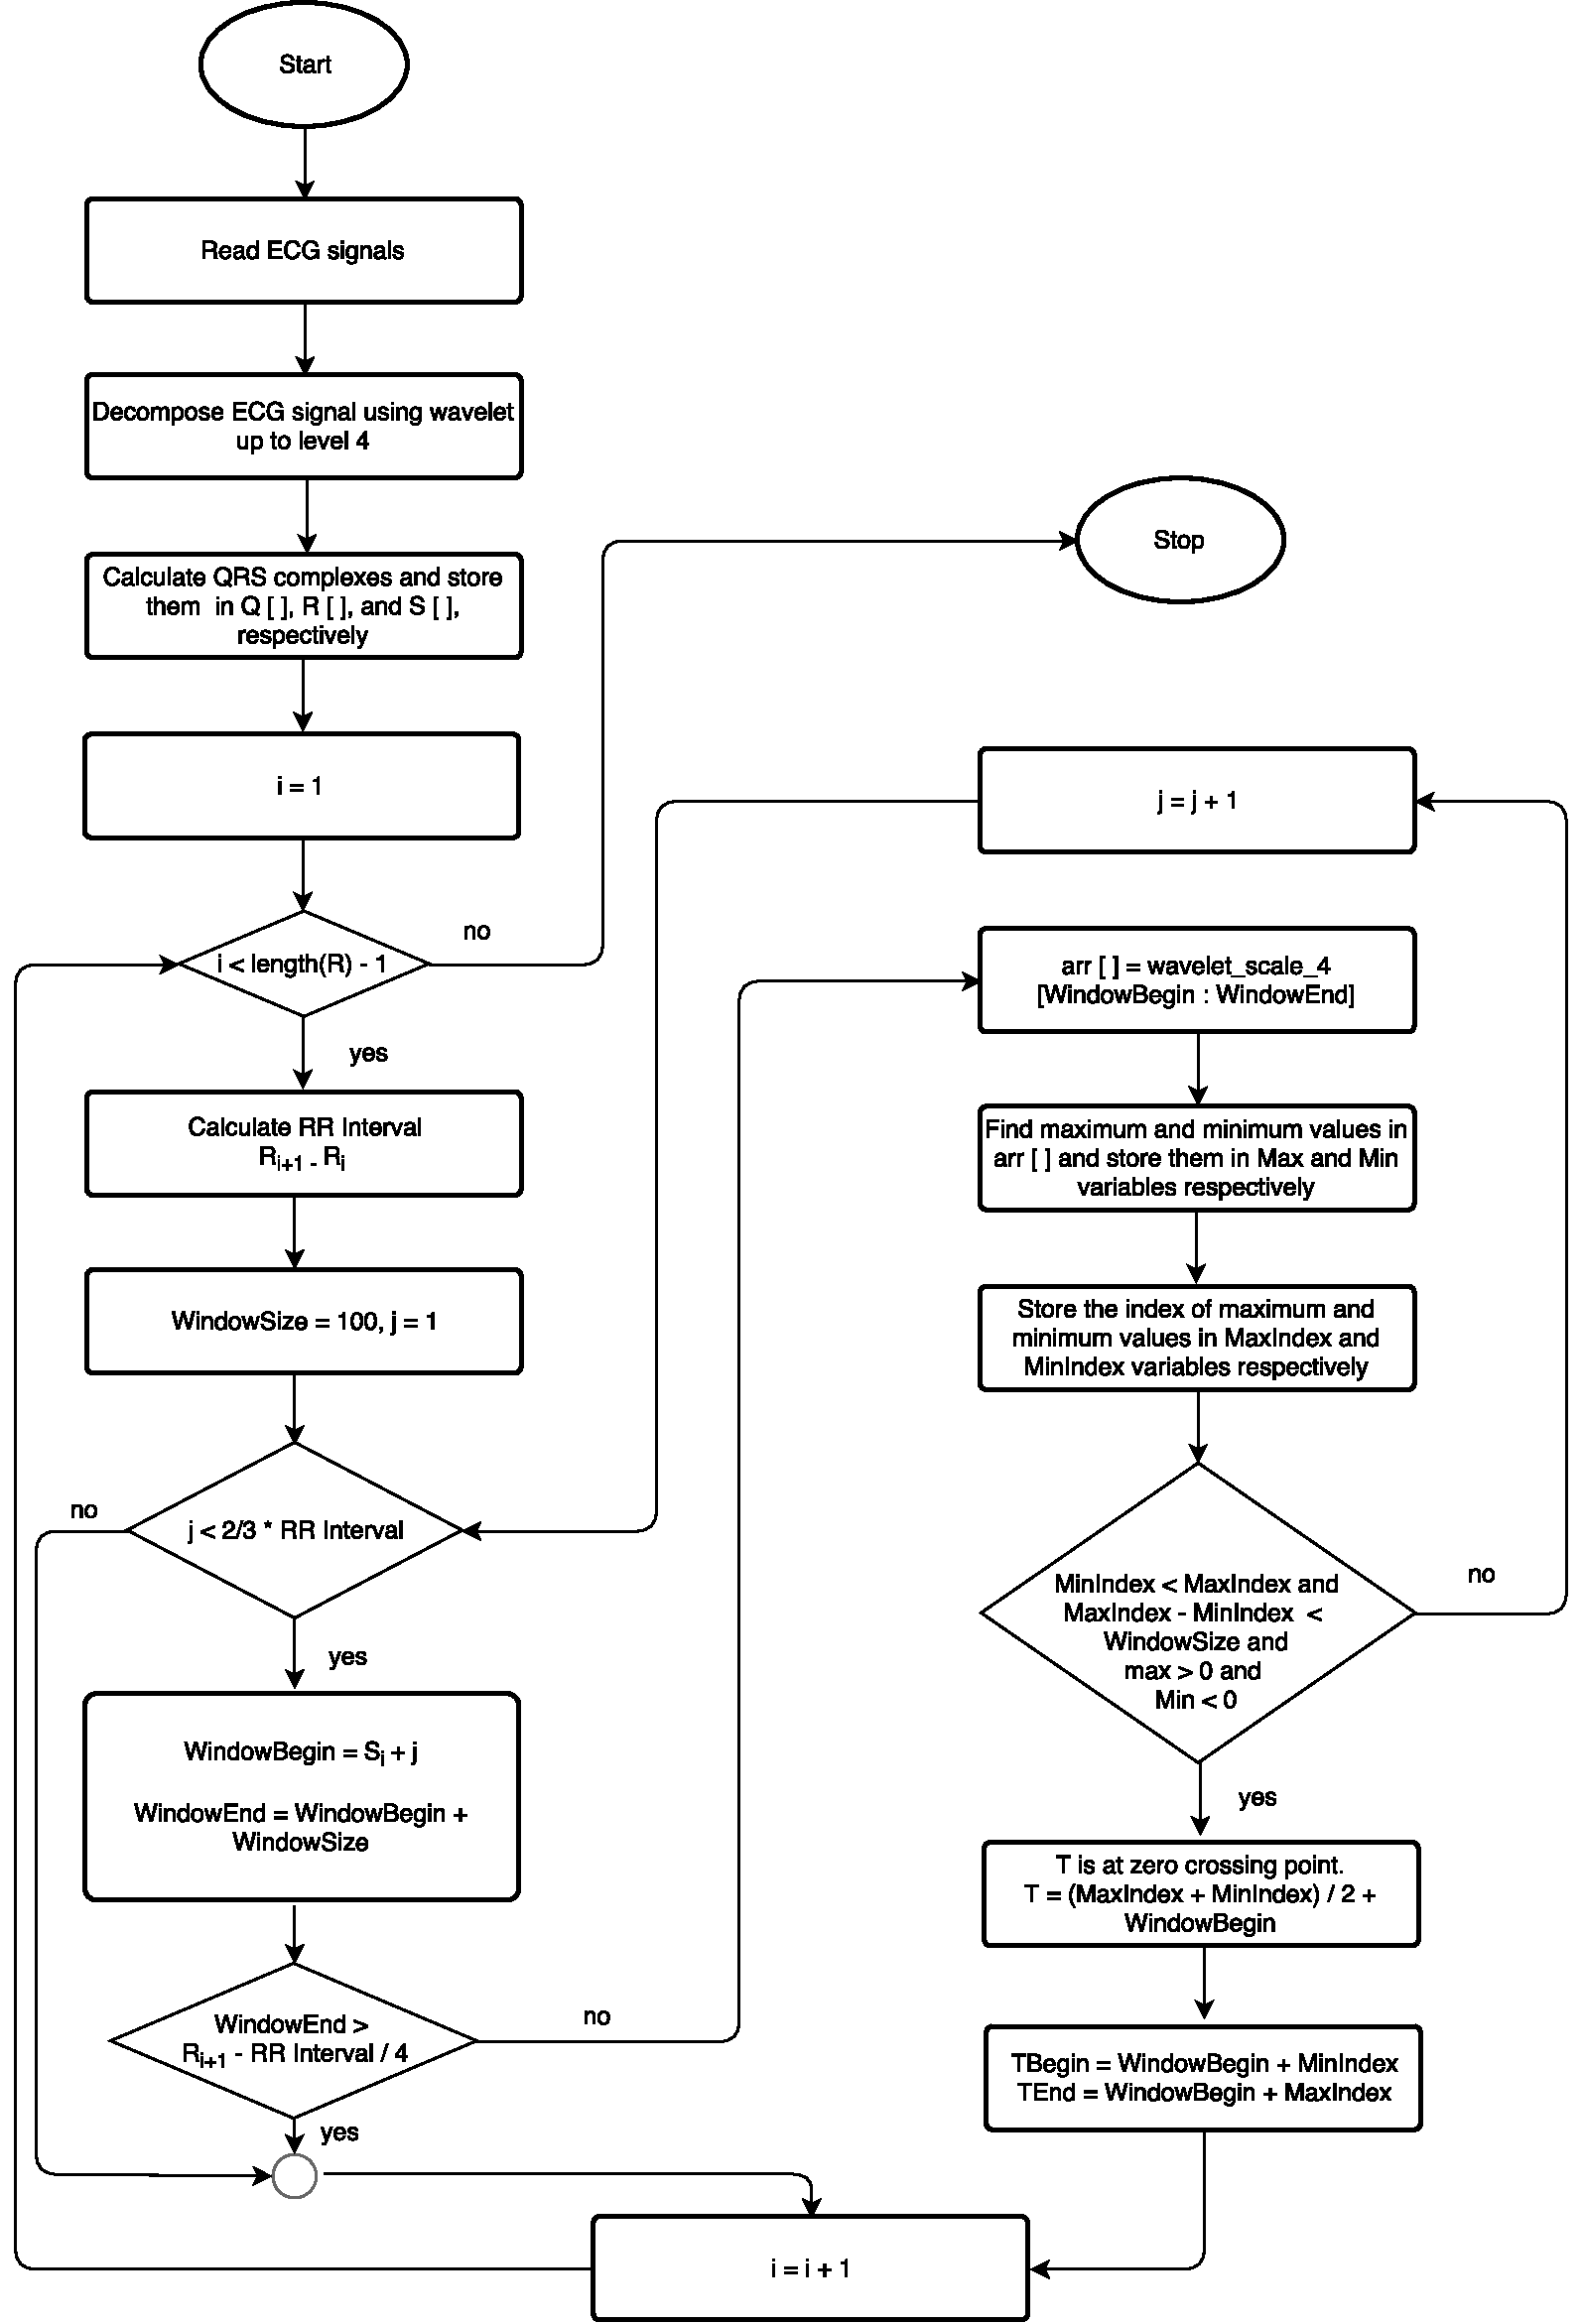
\includegraphics[width=25cm,height=22cm,keepaspectratio=true]{images/T_Wave.pdf}
	\caption{
		T wave flow chart.
	}
	\label{fig:t_peaks_flow_chart}
\end{figure}


\section{Heart Rate Calculation}
The heart rate is calculated by first counting the number of R peaks in a 10 seconds window and then multiply the count by 6 to get the heart rate.

\begin{center}
	$HeartRate = number\_of\_R\_peaks \times 6$
\end{center}

\section{Algorithm Execution on ECG Chair Data}
The data used in the development of ECG feature extraction algorithm is taken from MIT-BIH data set and the algorithm works great with that data set. To analyze the performance of algorithm on the ECG chair data that is used in the implementation of the system, the data is collected from the ECG chair and passed to the algorithm. It turns out that the algorithm works perfectly fine with this data as well. The original ECG signal can be seen in Figure \ref{fig:device_ecg_orignal} and the extracted features can be seen in Figure \ref{fig:device_ecg_feature_extraction}.

\begin{figure}[htpb]
	\centering
	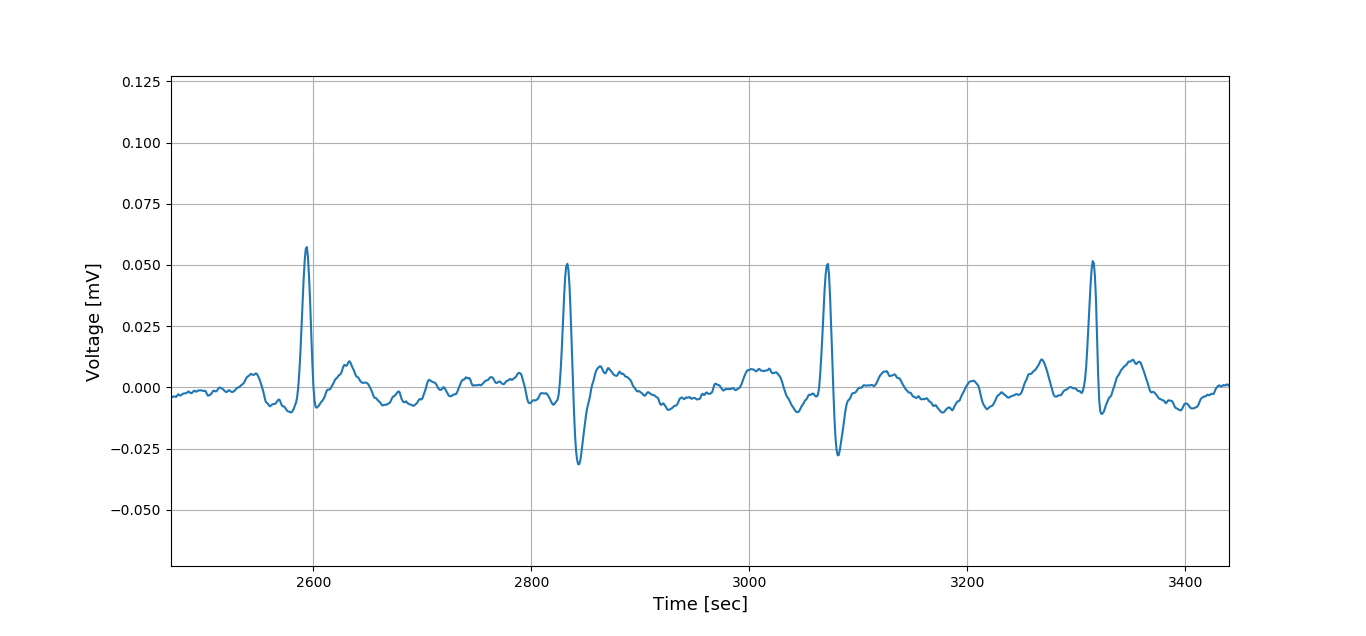
\includegraphics[width=15cm,height=15cm,keepaspectratio=true]{images/device_ecg_orignal}
	\caption{
		Original ECG chair signal.
	}
	\label{fig:device_ecg_orignal}
\end{figure}

\begin{figure}[htpb]
	\centering
	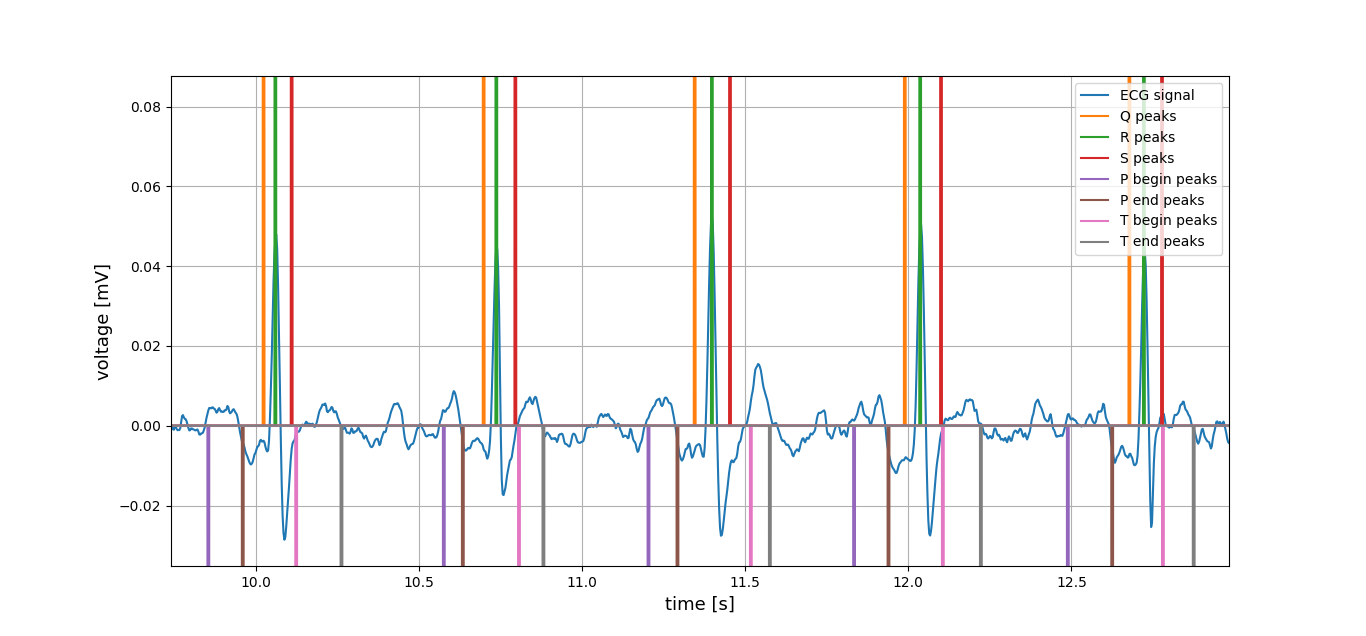
\includegraphics[width=15cm,height=15cm,keepaspectratio=true]{images/device_ecg_feature_extraction.png}
	\caption{
		Detected P,Q,R,S and T waves on the ECG chair signal.
	}
	\label{fig:device_ecg_feature_extraction}
\end{figure}



%**************
%* Deep Learning *
%**************

%\ihead{\headmark}
\chapter{Deep Learning}

Deep learning is a subfield of machine learning which is in fact, is a subfield of Artificial Intelligence (AI). Deep learning has emerged as one of the most exciting fields of computer science, and it keeps expanding its scope. It has been used in many technologies such as, in medical to identify the diseases, automatic game playing, self-driving cars, image recognition, natural language processing and many more. The reason why deep learning is successful in many different domains is its ability to understand multiple levels of representation of data. Its mean that, it not only has the ability to classify and predict but also has the ability to learn a different level of complexity. Before diving into deep learning, it is necessary to understand a broader field "machine learning".

\section{Machine Learning}

Machine Learning is a data analysis method \cite{bishop2006pattern}. It gives the computer the ability to learn from data without being explicitly instructed. By using different machine learning algorithms, it helps to find hidden insights of data and allow us to build models to make predictions. It can be classified into 2 categories \cite{machinelearningmastery}.

\begin{enumerate}
	\item Supervised Learning
	\item Unsupervised Learning
\end{enumerate}

\subsection{Supervised Learning}

In supervised learning, the labeled data is used to train the models. Here, labeled data represents that the input and output variables are known in advance. Thus, a supervised machine learning algorithm is used to come up with a mapping function which maps the input variables to the output variables. Learning is supposed to be stopped when the level of performance reaches the desired result. Supervised learning is generally divided into regression and classification.
\begin{itemize}
	\item \textbf{Regression}: A problem in which the output variable is a category.
	\item \textbf{Classification}: A problem in which the output variable is the real value.
\end{itemize}

\subsection{Unsupervised Learning}

In unsupervised learning, only the input variables are known and no corresponding output variables are known. Thus, there are no labels given and it is expected from unsupervised machine learning algorithm to find the structure in the data, i.e. finding hidden patterns to learn more about data. It is different from supervised learning in that the correct output value is not known. Unsupervised learning is generally divided into clustering and association.

\begin{itemize}
	\item \textbf{Clustering}: Group objects in such a way that the objects, which are similar to each other, placed in the same cluster.
	\item \textbf{Association}: Discover rules that define the large portions of the data such as people who buy product X may buy Y as well.
\end{itemize}

The objective of machine learning is to analyze the past and present data and predict or make a decision for the future data. In supervised learning, the basic workflow is to build a model, evaluate or tune a model and then deploy it in the production environment where it will do the predictions. The workflow can be seen in the figure.


\begin{figure}[htpb]
	\centering
	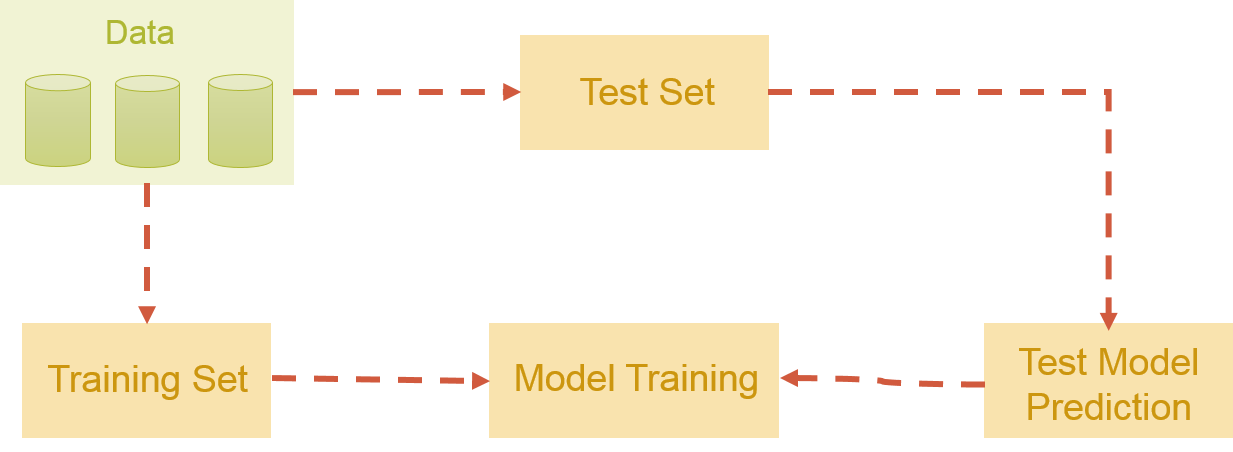
\includegraphics[width=12cm,height=10cm,keepaspectratio=true]{images/basic-ml-model.png}
	\caption{
		Basic supervised machine learning workflow.
	}
	\label{fig:basic-ml-model}
\end{figure}


Machine learning is generally powered by a huge amount of data which is generally referred aa Big Data. It is generally defined as a too big or complex data which cannot be processed on a single machine. As the data is growing day by day, the new tools are also required to process that big data on multiple machines and extract the useful insights from the data.


One of the problems with the traditional machine learning model is the feature extraction challenge. The model designer or the programmer need to specifically tell the model which features it should consider making a correct decision. The model heavily relies on the programmer's understanding of data and this was a huge burden on the programmers. For problems like object recognition, language translation, it was considered as a huge problem.

Deep learning comes into play to solve the problem of feature extraction. They have the capability to focus only on the right features by themselves by understanding as much data as possible, requiring very little input from the programmer. This feature of deep learning models makes it very powerful tool for the current machine learning era.




\section{Artificial Neural Networks}
Artificial neural networks (ANNs) are generally inspired by the biological neural networks that mimic brain functionality \cite{wiki:ann}. These systems generally learned by considering examples instead of specifically define rules for certain situations or cases. An ANN is a network of nodes called artificial neurons which are connected to other neurons using a link called \textit{synapse}. Each neuron gets the input, process the input and pass the output to the next neuron.
In the most basic state, an ANN consists of 3 layers:

\begin{enumerate}
	\item Input Layer
	\item Hidden Layer
	\item Output Layer
\end{enumerate}

\begin{figure}[htpb]
	\centering
	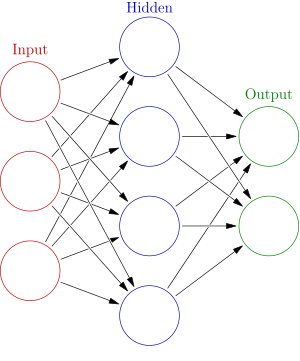
\includegraphics[width=6cm,height=10cm,keepaspectratio=true]{images/neural-net}
	\caption{
		An artificial neural network with its 3 basic layers, taken from \cite{wiki:ann}.
	}
	\label{fig:wiki:ann}
\end{figure}


\subsection{Artificial Neuron}
An artificial neuron is the most basic unit of ANN. It takes inputs and produces an output. Generally, the inputs are multiplied by some weights to specify which inputs are more important. The higher the value of weights, the more important they are. The inputs are shown as a, b, and c, and weights as $w_1$, $w_2$ and $w_3$ in figure \ref{fig:single-neuron}. After then the products are summed together and passed to the activation function. An activation function is a function which takes an input an generates an output based on a certain threshold. So, if the summed value is greater than the threshold value of that activation function, the output is produced or in other terms, the neuron fired else no output is produced and neuron does not fire.

\begin{figure}[htpb]
	\centering
	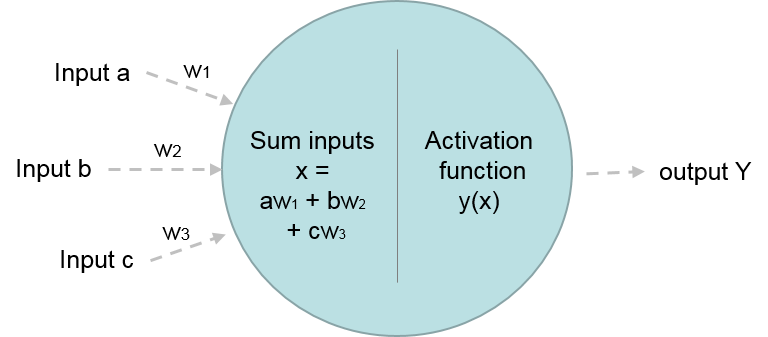
\includegraphics[width=10cm,height=10cm,keepaspectratio=true]{images/single-neuron}
	\caption{
		A single artificial neuron.
	}
	\label{fig:single-neuron}
\end{figure}

Artificial neurons adjust the weights as the learning proceeds and the process of finding weights is known as learning. ANN considers many different examples and finds the best possible combination of weights to provide the most accurate results. There are many other parameters involved as well to find a good combination of weights.

\subsection{Activation Function}

A function that takes an input and produces output based on threshold value is known as activation function \cite{ujjwalkarn}. There are many activation functions available. Few of them are:

\subsubsection{Sigmoid}
It takes a real value input and scales it to the range of 0 to 1. It is also known as the logistic function. It is represented as:

\begin{center}
	$y = \frac{1}{1 + e^{-x}}$
\end{center}

Another variation of the sigmoid function is softmax function which is used for multiclass classification.

\subsubsection{Tanh}
It takes a real value input and scales it to the range of -1 to 1. It is also a sigmoidal function as it also takes s-shaped.


\subsubsection{ReLU}
It stands for Rectified Linear Unit. It is the most used activation function as it is the ideal choice to be used in convolutional neural networks. It takes the real value input and all negative values are mapped to zero. It is represented as:

\begin{center}
	$f(x) = max(0, x)$
\end{center}

\begin{figure}[htpb]
	\centering
	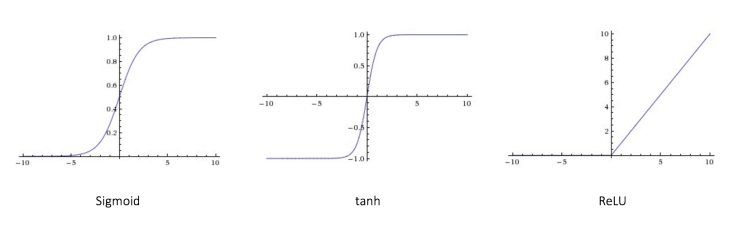
\includegraphics[width=15cm,height=10cm,keepaspectratio=true]{images/act-funcs}
	\caption{
		Activation functions, taken from \cite{ujjwalkarn}.
	}
	\label{fig:funcs}
\end{figure}

The graph of all the activation functions defined above can be seen in figure \ref{fig:funcs}.

\subsection{Convolutional Neural Network}
Convolutional neural network (CNN) is a class of deep neural network which uses multilayer perceptrons. It consists of an input layer, an output layer, and multiple hidden layers. The hidden layers can be convolutional, pooling or fully connected layer.


\subsubsection{Convolutional Layer}
In CNN, the first layer is always the convolutional layer. This layer applies a convolutional operation to the input and passes the output to the next layer. A filter (or sometimes referred as a kernel) is used which slides over all the area of the input and extract the features from it. The region where the filter is being applied at any instant of time is called as a receptive field. As the filter slides or convolves over the input signal, it multiples the filter with the original signal values (which can also be referred as element-wise multiplication) which results in a single value. The important point to note here is that this single result is just from a single receptive field. Therefore, the same operation will be carried out on other receptive fields by sliding the filter over the different areas of the input signal. The filter can slide for any unit and this sliding unit is known as stride. Every unique area of the input signal will produce an output and the combined output together is called as feature map or an activation map.  If we assume that, the input size is 32x32, the filter size is 5x5 and the stride is 1 unit, then the size of the activation map will be 28x28. In a 2D array, the filter can be moved in both directions.

\subsubsection{Pooling Layer}
Pooling layer is used to downsampled the convolutional layer output. There are several pooling options, for example, average pooling, L2-norm pooling, etc., but max polling is the most popular. This layer basically takes a filter of size 2x2 with the same stride size. It then applies the filter to the part of input and output the maximum number in that region. The same process is applied to the different sub-region by sliding the filter all over the input. By convolving the filter around the input, it drastically reduces the spatial size of the input. The example can be seen in the figure \ref{fig:maxpool}.

\begin{figure}[htpb]
	\centering
	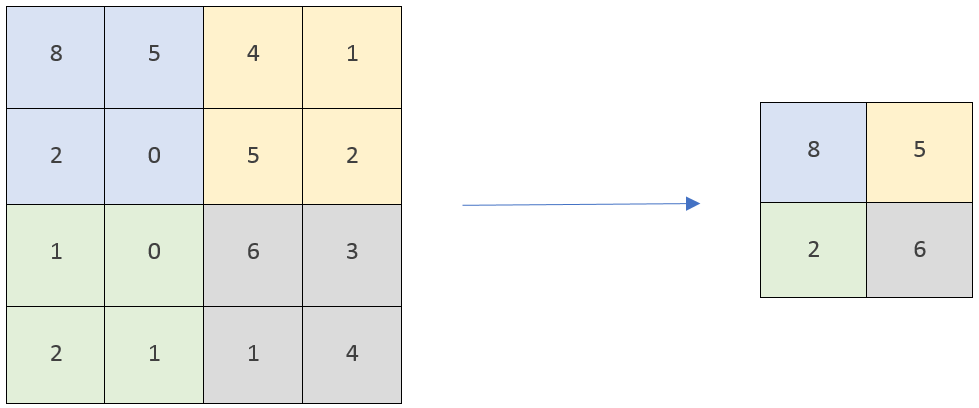
\includegraphics[width=12cm,height=10cm,keepaspectratio=true]{images/maxpool}
	\caption{
		Max pooling layer example.
	}
	\label{fig:maxpool}
\end{figure}

\subsubsection{Fully Connected Layer}
In fully connected layer, the neurons of one layer are connected to all the neurons of the other second layer, as it can be seen in figure 6. This layer can be seen in the regular neural network as well. The softmax function is applied to the output of the second layer to produce the probabilities for the classification of the input. 

\subsection{Keras}

Keras is an open source artificial neural network library written in python. It is very powerful and easy to use library to develop neural networks. It has a capability to run on top of TensorFlow, Microsoft Cognitive Toolkit (CNTK), or Theano, can run on both CPU and GPU. Before keras, it was really time-consuming to develop a network on TensorFlow or Theano and the aim to develop keras was to make it easy and fast to develop neural networks. Keras supports both convolutional neural networks and recurrent neural network, as well as a combination of both.

The model starts by defining the model as sequential using a \textit{Sequential()}, which is a linear stack of layers. Then the layers are added into the model using \textit{add()} method. Keras supports almost all kinds of layers. The input dimensions are needed to specify when the layers are added to the model. Once the layers are added, the model is compiled by using the \textit{compile()} method, which additionally needs 3 arguments.

\begin{itemize}
	\item Optimizer: To optimize the neural network, for example, rse, adagrad, adam, etc.
	\item Loss Function: This is the value that model tries to minimize to calculate the error, for example, categorical\_crossentropy, mse, etc.
	\item Metrics: It can be any existing metric or a custom defined metric function. But for classification problems metrics=['accuracy'] is recommended.
\end{itemize}

Then the model is trained by using the \textit{fit()} method. This method lets the model iterate over the data and find the most optimal neural network for the given data.

This library has been used for training the CNN for the identification of Cardiac Arrhythmias.

\subsection{Convolutional Neural Network for the Identification of Cardiac Arrhythmia}
A 6-layer Convolutional Neural Network (CNN) has been trained for the identification of an arrhythmia in an ECG signal. The trained model can detect 3 different kinds of arrhythmia namely:

\begin{enumerate}
	\item Normal
	\item Left bundle branch block (LBBB)
	\item Right bundle branch block (RBBB)
	\item Premature ventricular contraction (PVC)
\end{enumerate}

The CNN layers can be seen in the figure \ref{fig:cnn_model}.

\begin{figure}[htpb]
	\centering
	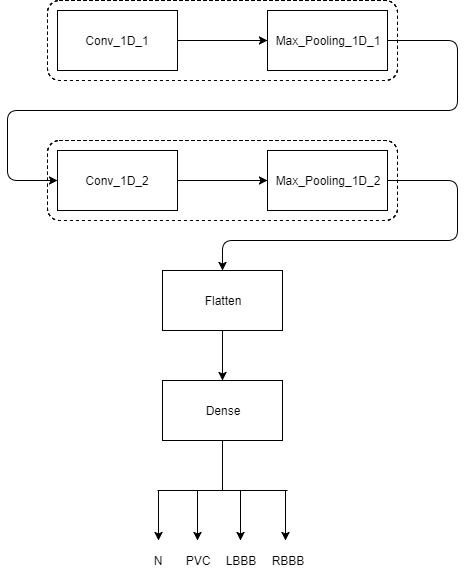
\includegraphics[width=20cm,height=15cm,keepaspectratio=true]{images/cnn_model}
	\caption{
		A 6-layer Convolutional Neural Network model for the identification of cardiac arrhythmia.
	}
	\label{fig:cnn_model}
\end{figure}


\begin{figure}[htpb]
	\centering
	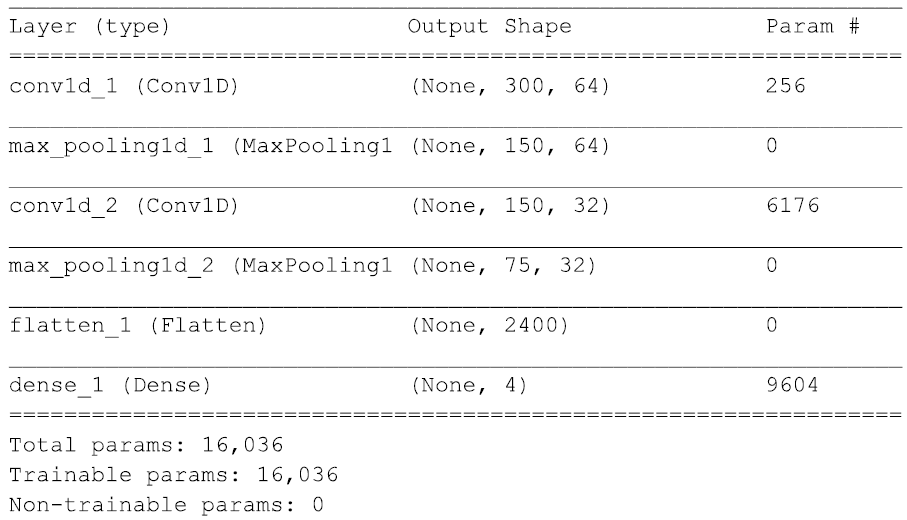
\includegraphics[width=12cm,height=10cm,keepaspectratio=true]{images/model_def_var}
	\caption{
		Layers used in the model and number of parameters to be optimized.
	}
	\label{fig:model_def_var}
\end{figure}

\subsubsection{Layers Explanation}
The 1st convolutional layer (Conv\_1D\_1) consists of 64 filters, whereas, the 2nd convolutional layer (Conv\_1D\_2) consists of 32 filters with a kernel of size 3. For both convolutional layers, Relu has been used as an activation function each followed by a MaxPooling layer. The batch size of 1000 was used for the training, along with the Adam algorithm to optimize the CNN. Since the model is trained for performing the classification of an ECG signal, therefore, categorical cross-entropy loss function was used for calculating the loss of training and validation. After performing the convolutions, the flattening and dense layer has been used followed by a softmax activation function to produce the final probabilities with 4 classes.


The model was trained and tested for the several no. of iterations ranging from 10 to 100. The best model was found after the 20 iterations. After that, the model remained stable with the slight improvement in the training as well as in the validation accuracy. The training and validation accuracy can be seen in the figure \ref{fig:acc_val}.

\begin{figure}%
	\centering
	
	\subfigure[][]{%
		\label{fig:ex3-c}%
		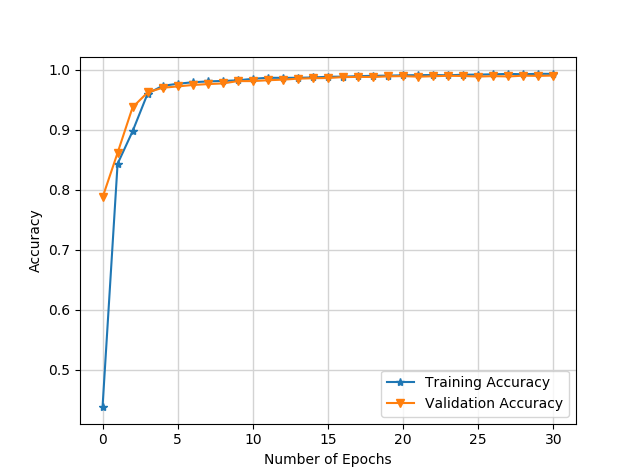
\includegraphics[height=4in]{images/acc}}%
	\hspace{8pt}%
	\subfigure[][]{%
		\label{fig:ex3-d}%
		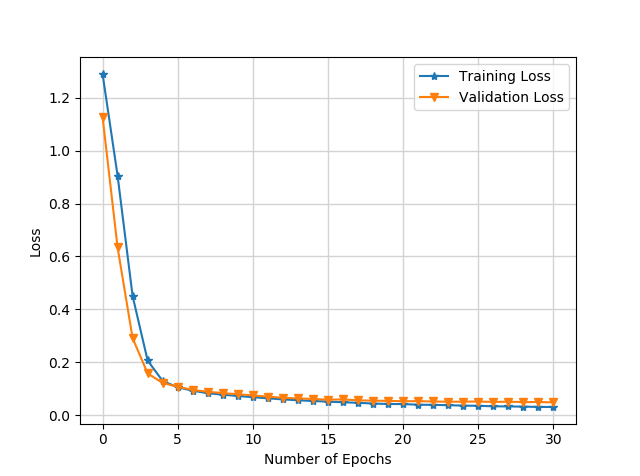
\includegraphics[height=4in]{images/val}}%
	\caption[A set of four subfigures.]{
		\subref{fig:ex3-c} Training and validation accuracy results; and,
		\subref{fig:ex3-d} Training and validation loss of CNN model for 30 iterations.}%
	\label{fig:acc_val}%
\end{figure}


\subsubsection{Results}
The CNN model has achieved an accuracy of 99.2\% on MIT-BIH dataset. Total 16,415 ECG signals were extracted from the MIT-BIH dataset, out of which 10,998 (67\% of the total signals) were used for the training, and the remaining 5,417 (33\% of the total signals) were used for the testing of the model. The types count for training and testing data can be seen in Tables \ref{tab:train_count} and \ref{tab:test_count} respectively. 

\renewcommand{\arraystretch}{2}
\begin{table}
	\caption{Training data.} \label{tab:train_count}
	
	\begin{center}
		\begin{tabular}{ | l | r | }
			\hline
			\textbf{Type} & \textbf{Count} \\ \hline
			Normal & 3,352 \\ \hline
			LBBB  & 2,641  \\ \hline
			RBBB  & 2,498  \\ \hline
			PVC  & 2,507  \\ \hline
			\textbf{Total}  & \textbf{10,998}  \\ \hline
		\end{tabular}
	\end{center}
	
\end{table}


\renewcommand{\arraystretch}{2}
\begin{table}
	\caption{Test data.} \label{tab:test_count}
	
	\begin{center}
		\begin{tabular}{ | l | r | }
			\hline
			\textbf{Type} & \textbf{Count} \\ \hline
			Normal & 1,648 \\ \hline
			LBBB  & 1,308  \\ \hline
			RBBB  & 1,285  \\ \hline
			PVC  & 1,176  \\ \hline
			\textbf{Total}  & \textbf{5,417}  \\ \hline
		\end{tabular}
	\end{center}
	
\end{table}

During the testing of the model, 42 ECG signals were classified wrong out of 5,417 ECG signals. The false predicted results can be seen in Table \ref{tab:false_pred_count}. In table, $a \rightarrow b$ means is that $a$ was classified as $b$.






\renewcommand{\arraystretch}{2}
\begin{table}
	\caption{False Prediction Counts.} \label{tab:false_pred_count}
	
	\begin{center}
		\begin{tabular}{ | l | r | }
			\hline
			\textbf{False Prediction} & \textbf{Count} \\ \hline
			0 $\rightarrow$ 1  & 1   \\ \hline
			0 $\rightarrow$ 2  & 1  \\ \hline
			0 $\rightarrow$ 3  & 3  \\ \hline
			1 $\rightarrow$ 3  & 6  \\ \hline
			2 $\rightarrow$ 0  & 5  \\ \hline
			2 $\rightarrow$ 3  & 3  \\ \hline
			3 $\rightarrow$ 0  & 9  \\ \hline
			3 $\rightarrow$ 1  & 12 \\ \hline
			3 $\rightarrow$ 2  & 2  \\ \hline
			\textbf{Total}   & \textbf{42}  \\ \hline
		\end{tabular}
	\end{center}
	
\end{table}


%**************
%* visualization *
%**************

%\ihead{\headmark}
\chapter{Visualization}


\makeatletter
\renewcommand{\@chapapp}{}% Not necessary...
\newenvironment{chapquote}[2][2em]
{\setlength{\@tempdima}{#1}%
	\def\chapquote@author{#2}%
	\parshape 1 \@tempdima \dimexpr\textwidth-2\@tempdima\relax%
	\itshape}

\makeatother

\begin{center}
\begin{chapquote}{}
	``A picture is worth a thousands words.''
\end{chapquote}
\end{center}

Raw numbers to the users do not make sense and therefore, require necessary tools to display the result. Visualization allows us to see the broader aspects of complex data by showing the data in graphical formats. It really helps in capturing the user's attention and engage him through out the process. Complex data that could easily be ignored, can still be recognized and captured the attention of the user in a graphical reports \cite{quora:Sulakshana}.

The visualization tool Grafana has been set up for displaying the real-time data received from the sensors. All devices send the data in real-time which first get stored in Influxdb and then Grafana tool loads the data from there and display it on the graph. 

\section{Grafana}
Grafana is an open source real-time visualization tool for analytics and monitoring. It is one of the best tools for time series analytics, therefore, it is used for visualizing the real-time graphs from sensor devices. It can be used for any kind of application analytics, for example, industrial sensors, home automation, hospitals, weather reports etc. It allows to connect to many data sources available and pull data from it to do the analytics or the visualization. The most commonly used data sources these days are:

\begin{itemize}
	\item Elasticsearch
	\item InfluxDB
	\item Graphite
	\item Prometheus  
\end{itemize}

It allows us to connect to these data sources on just few click which makes it very convenient. Multiple dashboards can be created in grafana to view different dimensions of the data. It also provides multiple tools for creating graphs in different fashion and styles which can be added to dashboards.

\section{InfluxDB}
 Since the sensor data is always time critical, therefore, a time series database is required for storing the data. InfluxDB is one of the best time series database available, therefore, it has been chosen for storing the sensors data. 
 
 It is very easy install and manage, and does not require other dependencies to run. It also provides an HTTP/HTPPS interface to read and write data from the database. The retention policy can be set on the database to manage space conveniently. The basic terms in InfluxDB are:
 
 \begin{itemize}
 	\item Database name
 	\item Measurement (same as table name in traditional databases)
 	\item Tags (to filter data)
 	\item Fields (actual data values)
 \end{itemize}
 
 The fields are generally used in a key value pair, with a timestamp field. Only one point can be stored at any specific timestamp. The precision of a single field can be in s, ms, $\mu$s, ns. If the field does not contains a timestamp field, then InfluxDB will generate a timestamp automatically.
 
 Another reason for choosing the influxDB is that, it is really easy to configure grafana for using influxDB as a data source.



%**************
%* conclusion *
%**************

% !TEX root = ../main.tex

%\chapter{Fazit}
\chapter{Conclusion}
\label{sect:conclusion}
		
% Gehe auf Ziel, Aufgabenstellung aus Einleitung ein und wiederhole zusammenfassend, wie die Aufgabenstellung erfüllt wurde und was die Ergebnisse sind.
% Adress the aim and the conceptual formulation of the assignment from the introduction directly and summarise how the formulated goals were reached (or not).

The aim of this document was to provide students at the end of their studies with a template for their written thesis.
Due to the common lack of experience in the field of academic writing this work is intended to provide a template for structured writing.
Therefore, this entire document is structured as a thesis should usually be.

Moreover it provides some hints how citations should be used and how figures should be dealt with to achieve high quality versions of latex documents.
In contrary to this sentence, a conclusion should not introduce new information, about the topics discussed before, which has not yet been presented.

The following (optional) section provides some further ideas for potential extension of this work.

%\section{Ausblick} %(optional)
\section{Future Work} % (optional)

% Wie könnte es weiter gehen? Dieser Abschnitt kann auch in einem eigenen Kapitel vorhergehen.
% Short description how this work could be pursued. This can be done in a separate chapter preceding the conclusion, too.

There are many possible ways how this short document could be extended in the future.
One may think of additional explanations regarding latex and its use, with the extend to an entire latex tutorial.
A further extension could be the definition of helpful latex commands or a documentation on commonly used latex commands and packages.
%*************
%* Hauptteil *
%*************
 
%%\ihead{\headmark}
\chapter{Allgemeine Bestimmungen f�r Abschlussarbeiten}
Die allgemeinen Bestimmungen f�r Studien- und Diplomarbeiten bzw. Bachelor- und Masterarbeiten regeln die f�r den jeweiligen
Studiengang geltenden Pr�fungsordnungen (DPO, BPO bzw. MPO). F�r den Fachbereich
Elektro- und Informationstechnik ist die jeweils G�ltige auf den Internet Seiten des Fachbereichs
(\url{http://www.fb6.rwth-aachen.de/}) verf�gbar. Dieses Merkblatt enth�lt
erg�nzende Hinweise f�r die praktische Durchf�hrung der Arbeit.


\section{Bachelorarbeit}
Die Bachelorarbeit ist eine Pr�fungsarbeit innerhalb der Fakult�t, die die wissenschaftliche
Ausbildung zum Bachelor of Science abschlie�t. Neben der schriftlichen Ausarbeitung schlie�t
die Bachelorarbeit auch einen Vortrag �ber die Ergebnisse mit ein. 

Die Ausgabe des Themas erfolgt formal �ber die Vorsitzende bzw. den Vorsitzenden des
Pr�fungsausschusses der Fakult�t f�r Elektro- und Informationstechnik. Praktisch erfolgt die
Themenstellung der Bachelorarbeit von einem der Fakult�t angeschlossenen Lehrstuhl. Die
Bearbeitungszeit f�r die Bachelorarbeit betr�gt bei Vollzeitarbeiten drei Monate und bei Aufgaben die
in Teilzeit bearbeitet werden sechs Monate. Thema und
Aufgabenstellung m�ssen so beschaffen sein, dass die zur Bearbeitung vorgegebene Frist eingehalten
werden kann. Das Thema kann nur einmal und nur innerhalb des ersten Monats der
Bearbeitungszeit zur�ckgegeben werden. Im Einzelfall kann der Pr�fungsausschuss auf begr�ndeten
Antrag der Kandidatin bzw. des Kandidaten die Bearbeitungszeit ausnahmsweise um bis zu vier Wochen
verl�ngern. Die Arbeit inklusive Abschlussvortrag wird mit 12 CP bewertet.

Das Thema der Bachelorarbeit kann erst dann an den Bewerber ausgegeben werden, wenn er 120 CP erbracht hat. 
N�heres regelt die jeweilige Bachelorpr�fungsordnung. Zum Anfertigen einer Bachelorarbeit muss sich der Bewerber beim Zentralen
Pr�fungsamt (ZPA) der RWTH anmelden.


\section{Masterarbeit}
Auszug aus der Master Pr�fungsordnung \cite{MPO-10-2010}:
\begin{quote}
\begin{enumerate}\setlength{\itemsep}{0pt}
\setlength{\parsep}{0pt}
\item Die Master-Arbeit besteht aus einer schriftlichen Arbeit der Kandidatin bzw. des Kandidaten.
Sie soll zeigen, dass die Kandidatin bzw. der Kandidat in der Lage ist, ein Problem innerhalb
einer vorgegebenen Frist nach wissenschaftlichen Methoden unter Anleitung selbstst�ndig
zu bearbeiten.
\item Die Master-Arbeit kann von jeder bzw. jedem in Forschung und Lehre in der Fakult�t f�r
Elektrotechnik und Informationstechnik an der RWTH t�tigen Professorin bzw. Professor
ausgegeben und betreut werden. Lehrbeauftragte und wissenschaftliche Mitarbeiterinnen
bzw. Mitarbeiter k�nnen bei der Betreuung mitwirken. In Ausnahmef�llen kann die Master-
Arbeit mit Zustimmung des Pr�fungsausschusses au�erhalb der Fakult�t bzw. au�erhalb
der RWTH ausgef�hrt werden, wenn sie von einer der in Satz 1 genannten Personen betreut
wird (s. Anlage 4).
\item Auf besonderen Antrag der Kandidatin bzw. des Kandidaten sorgt die bzw. der Vorsitzende
des Pr�fungsausschusses daf�r, dass sie bzw. er zum vorgesehenen Zeitpunkt das Thema
einer Master-Arbeit erh�lt. Der Kandidatin bzw. dem Kandidaten ist Gelegenheit zu geben,
f�r das Thema Vorschl�ge zu machen.
\item Die Master-Arbeit kann im Einvernehmen mit der Pr�ferin bzw. dem Pr�fer wahlweise in
deutscher oder englischer Sprache abgefasst werden.
\item Die bzw. der Vorsitzende des Pr�fungsausschusses teilt der Kandidatin bzw. dem Kandidaten den Abgabetermin mit. Der Zeitpunkt der Ausgabe sowie die Themenstellung sind aktenkundig zu machen.
\item Die Bearbeitungszeit f�r die Master-Arbeit betr�gt maximal sechs Monate. Der Umfang der
schriftlichen Ausarbeitung sollte ohne Anlage 80 Seiten nicht �berschreiten. Das Thema kann nur einmal und nur innerhalb des ersten Monats der Bearbeitungszeit zur�ckgegeben
werden. Ausnahmsweise kann der Pr�fungsausschuss im Einzelfall auf begr�ndeten Antrag
der Kandidatin bzw. des Kandidaten und bei Bef�rwortung durch die Aufgabenstellerin bzw.
den Aufgabensteller die Bearbeitungszeit um bis zu sechs Wochen verl�ngern.
\item Die Ergebnisse der Master-Arbeit pr�sentiert die Kandidatin bzw. der Kandidat im Rahmen
eines Master-Vortragskolloquiums.
\end{enumerate}
\end{quote}


\section {Auswahl eines Themas}
Die �blicherweise ausgegebenen Themen k�nnen nach Schwerpunkten
unterteilt werden. Dies sind Arbeiten in
\begin{itemize}
 \item theoretischer Richtung (Modellbildung und Berechnungen, Simulation, Methoden)
 \item experimenteller Richtung (Messtechnik, Messungen und Analyse der Messergebnisse)
 \item konstruktiver Richtung (Entwurf, Aufbau, Konstruktion)
\end{itemize}


Viele Arbeiten sind Teile der am Institut laufenden Forschungsarbeiten. Unter Umst�nden sind es
aber auch eigenst�ndige Themen, wie z.B. Planung und Aufbau von Praktikumsversuchen oder besonderen
Ger�ten. Alle Arbeiten erfordern eine gewisse Einarbeitungszeit. Es wird empfohlen, die
Wahlvorlesungen rechtzeitig auch im Hinblick auf beabsichtigte Themenbereiche von Studien- und 
Diplomarbeiten bzw. Bachelor- und Masterarbeiten auszuw�hlen. Die Einarbeitung in ein bestimmtes 
Gebiet der Abschlussarbeit ist ein wesentlicher Bestandteil der selbst�ndig durchzuf�hrenden Arbeiten im Studium mit einem
meist besonders gro�en Lerneffekt. Es empfiehlt sich, fr�hzeitig ein methodisches Vorgehen zu
�berlegen und in Absprache mit dem Betreuer einen Terminplan aufzustellen. Au�erdem geh�rt ein
ausf�hrliches Literaturstudium zur Einarbeitung. Die Auswahl des Themas selbst h�ngt weitgehend vom
Interesse des Studenten ab. Man sollte sich zuerst �berlegen, welche Ger�te oder Anlagen oder
welche theoretischen Methoden man gerne, auch im Hinblick auf den sp�teren Beruf, kennen lernen m�chte. Dabei ist es empfehlenswert wenn die Themen von Bachelor- und Masterarbeit in verschiedenen Bereichen liegen,
um sich so in einem gr��eren "`Spektrum"' auszubilden. Diese Chance an der Universit�t sollte unbedingt genutzt werden.

\chapter{Arbeitsbeginn}
Als Termin f�r den Beginn der Arbeit gilt die Aush�ndigung der schriftlich formulierten Aufgabe.
Der Student erh�lt am Lehrstuhl notwendige Arbeitsmaterialien mit Ausnahme von Schreib- und
Zeichenmaterial. Ausgegebene Ger�te d�rfen nicht ohne Erlaubnis durch den Betreuer aus dem
Institutsbereich entfernt werden. Falls erforderlich, wird ein fester Arbeitsplatz zugewiesen. Die
Schl�ssel zum Zugang der in Anspruch genommenen Einrichtungen (Rechner u.�.) werden gegen
Unterschrift und unter Hinweis auf die notwendigen Konsequenzen bei Verlust (z.B. �nderung der
gesamten Schl�sselanlage) ausgeh�ndigt.


\section{B�cher}
B�cher aus Institutsbest�nden d�rfen nicht aus den R�umen des Instituts entfernt werden, es sei
denn, ein Mitarbeiter hat dies explizit gestattet. In diesem Falle ist im  Sekretariat ein
Entleihschein zu hinterlegen. Die maximale Entleihzeit betr�gt zwei Wochen. Danach sind die B�cher
umgehend an den betreuenden Assistenten zur�ckzugeben. Einige der am Lehrstuhl vorhandenen B�cher
sind Privatbesitz (z.B. von Prof. Leonhardt). Diese d�rfen nur nach expliziter Erlaubnis des
Besitzers entliehen werden.

\section{Ablauf der Arbeit}
Zur eigenen Planung und �berwachung hat der Bearbeiter bei der Bachelor- und Studienarbeit sp�testens 3 Wochen
bzw. bei der Master- und Diplomarbeit 6 Wochen nach Beginn der Arbeit ein Arbeitsprogramm und einen Terminplan
zu erstellen. Dieser ist mit dem betreuenden wissenschaftlichen Mitarbeiter abzusprechen. Bei einer
Master- bzw. Diplomarbeit folgt darauf der Einf�hrungsvortrag (siehe Abschnitt~\ref{sec:vortrag}).

W�hrend der gesamten Arbeit hat der Student einen st�ndigen Kontakt zu dem betreuenden
wissenschaftlichen Mitarbeiter zu halten. Gespr�chstermine (in der Regel mindestens f�nf) sind
aus eigener Initiative des Studenten mit dem Betreuer zu vereinbaren.

\section{Der Einf�hrungsvortrag\label{sec:vortrag}}
Der Einf�hrungsvortrag sollte bei Master- bzw. Diplomarbeiten innerhalb der ersten 6 Wochen gehalten werden. Hier soll der Student
mit eigenen Worten eine Einf�hrung in die Themenstellung seiner Arbeit geben. Des Weiteren
soll die geplante Vorgehensweise mit Projektplan erl�utert werden. Der Projektplan umfasst dabei
sowohl die \textbf{inhaltliche} (welche (Teil)-Ergebnisse sollen erreicht werden), die
\textbf{terminliche} (wann sollen die definierten Arbeitspakete abgeschlossen werden) und auch die
\textbf{finanzielle} (welche Investitionen sind erforderlich) Strukturierung der Arbeit. Der
Vortrag sollte einen Umfang von 10 Minuten haben und nicht mehr als 6 Folien enthalten.

\section{Arbeitsende}
Bachelor-, Master- und Diplomarbeiten sind von Studierenden der Fakult�t f�r Elektrotechnik und Informationstechnik sp�testens am letzten Tag des Bearbeitungszeitraums (siehe schriftliche Aufgabenstellung) im Sekretariat des Lehrstuhls abzugeben. F�llt dieser Termin auf ein Wochenende, einen Feiertag oder sonstige dienstfreie Tage, so gilt der n�chste Arbeitstag als Abgabetermin. Informatiker geben ihre Diplomarbeiten im Zentralen Pr�fungsamt ab. Studienarbeiten werden ebenfalls im Sekretariat des
Lehrstuhls abgegeben.

\begin{figure}[!ht]
	\centering
	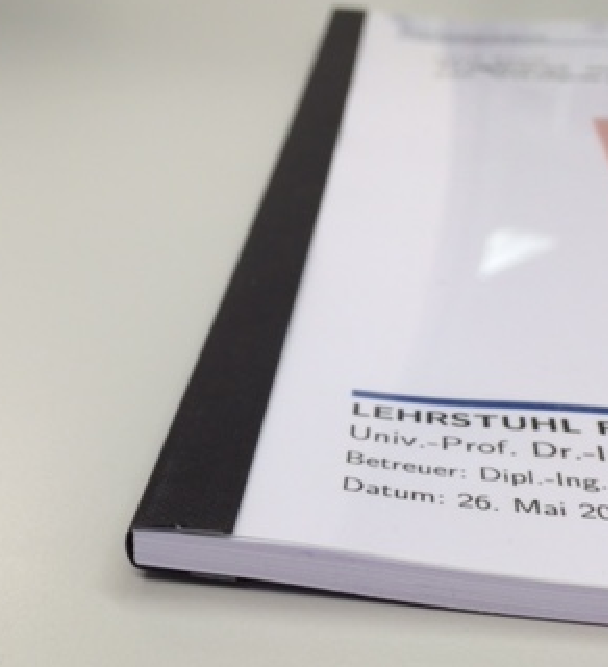
\includegraphics[scale=0.6]{images/leimbindung}
	%% Reihenfolge der Befehle wichtig: zuerst die \caption, danach das \label
	\caption{Leimbindung}
	\label{fig:Leimbindung}
\end{figure}
Insgesamt sind bei der Abgabe zwei Exemplare der Arbeit in Leimbindung (siehe Abb.~\ref{fig:Leimbindung}) einzureichen. Von diesen muss eines das offizielle, unterschriebene und im Sekretariat bereitliegende Deckblatt als vorderste Seite verwenden.
Umfangreichere Anh�nge, die nicht zusammen mit dem Hauptteil der Arbeit gebunden werden k�nnen, m�ssen nicht unbedingt in einer Leimbindung eingereicht werden; hier kann auch ein Leitz-Ordner (feste Struktur, wei�es R�ckenschild) verwendet werden.
Der Druck der Arbeit kann in Graustufen (Schwarzwei�) oder Farbe erfolgen. Im Fall des Schwarzwei�drucks m�ssen Grafiken derart gestaltet sein, dass alle Informationen ohne Farbe erkennbar sind.


Von allen Texten, Bildern, Programmen, Messdaten, Vortr�gen und sonstigen im Rahmen der Arbeit entstandenen Daten muss eine Sicherungskopie auf einem
archivierbaren Datentr�ger (z.B. CD, DVD) erstellt und in jede Arbeit eingelegt
werden. Zus�tzlich muss die schriftliche Arbeit in elektronischer Form als Postscript- und
PDF-Datei sowie im Original-Erstellungsformat (\LaTeX\ , Word, etc...) abgegeben werden. Die Kosten, die bei der Herstellung der Abgabeexemplare anfallen (Kopien/Binden/etc...), gehen im Regelfall zu Lasten des Studenten. Bei Abschluss der Arbeit sind alle Ger�te, B�cher, Schl�ssel u.�. zur�ckzugeben. Erst nach erfolgter R�ckgabe der genannten Materialen, der �bergabe des Datentr�gers und der Pr�sentation des abschlie�enden Seminarvortrags kann die Note in die Pr�fungsakte eingetragen werden. Bei Bachelor-, Master- und Diplomarbeiten wird das Datum der Abgabe der schriftlichen Ausarbeitung in die Pr�fungsakte eingetragen, nicht das Datum des evtl. sp�teren Seminarvortrags.


\chapter{Abfassung der schriftlichen Arbeit}
Als Ergebnis der Arbeit ist ein schriftlicher maschinengeschriebener Bericht
vorzulegen. Dieser Bericht soll f�r einen unvorbereiteten, aber fachkundigen Leser leicht
verst�ndlich sein. Dabei ist auch von m�glichst kompakten Formulierungen und Darstellungen Gebrauch
zu machen. F�r die L�nge der schriftlichen Ausarbeitung sind bei einer Studienarbeit etwa 40
Seiten, bei einer Bachelorarbeit etwa 50 Seiten und bei einer Diplomarbeit ca. 60 Seiten (ohne Anhang) 
anzustreben. Dies sind nat�rlich nur Richtwerte, aber eine deutlich l�ngere Arbeit (ohne dass der Inhaltliche 
Gehalt dies erfordert) wird nicht zwangsl�ufig besser beurteilt. Hingegen wird eine k�rzere auch nicht schlechter
bewertet, wenn daf�r auf verl�ngernde Prosa verzichtet wird.

Es wird empfohlen, den Text der Arbeit unter Verwendung g�ngiger Textverarbeitungsprogramme auf
wei�es Papier DIN A4 zu schreiben. Der R�nder sollten umlaufend mindestens 2,5 cm breit sein und es
sollte eine 1 bis 1,2-zeilige Schreibweise in 12pt Schrift gew�hlt werden. Eine \LaTeX\ Vorlage steht in Form 
des Quelltextes des vorliegenden Dokumentes zur Verf�gung.

Vom Lehrstuhl k�nnen keine Rechner speziell f�r die Abfassung der schriftlichen Arbeit zur
Verf�gung gestellt werden. Soweit Kapazit�t verf�gbar, k�nnen jedoch die Rechner in den
Arbeitsr�umen benutzt werden.
\clearpage



\section{Gliederung der Arbeit\label{sec:kap_seiten}}
Typischerweise enth�lt eine wissenschaftliche Arbeit die im folgenden aufgef�hrten Abschnitte:

\begin{tabular}{lcll}
  Aufgabenstellung (wird vom Institut erstellt)   &\hspace{3cm} & &\\
  Erkl�rung der Selbst�ndigkeit &&&\\
  Zusammenfassung &  & &i \\
  Inhaltsverzeichnis & && ii\\
  Verwendete Symbole& & &iv\\
  \\
  1. Einf�hrung & &Seite& 1 \\
  2. Grundlagen&&& 3 (z.B.)\\
  \hspace{5mm} 2.1 & & &.       \\
  \hspace{10mm} 2.1.1& & &. \\
  \hspace{10mm} 2.1.2& & &.\\
  \hspace{20mm} a)\\
  \hspace{20mm} b)\\
  \hspace{5mm} 2.2& & &.\\
  \hspace{5mm} 2.3& & &.\\
  .\\
  .\\
  5. Ergebnisse& & &.\\
  6. Zusammenfassung und Ausblick&&& 60 (z.B.)\\
  Literaturverzeichnis &&&63\\
  Tabellenverzeichnis (optional)\\
  Bilderverzeichnis (optional)\\
  Anhang\\
  A\\
  B\\
  .\\
  .\\
\end{tabular}


Die Aufteilung der Abschnitte sollte so gew�hlt werden, dass alle inhaltlichen Abschnitte (also
Grundlagen bis Ergebnisse) in etwa den gleichen Seitenumfang haben und nicht weniger als 15 Seiten
umfassen. Die Untergliederung sollte nicht �bertrieben werden. In der Regel ist eine Aufgliederung
bis in die dritte Ebene (z.B. 2.1.1) hinreichend.




\section{Zusammenfassung}
Am Anfang der Arbeit steht eine kurze Zusammenfassung mit einer maximalen L�nge von einer
halben Seite. Darunter sind bis zu f�nf Schl�sselw�rter f�r die Arbeit anzugeben. Wenn
m�glich, ist die Zusammenfassung ("`abstract"') zus�tzlich auch in englischer Sprache anzugeben.

\section{Inhaltsverzeichnis}
Das Inhaltsverzeichnis soll entsprechend DIN 1421 in gestaffelter Dezimalgliederung mit
arabischen Ziffern aufgestellt werden und die zu den Abschnitten geh�rigen Seitenangabe
enthalten. Als Beispiel kann das Inhaltsverzeichnis dieses Dokumentes herangezogen werden.
Die einleitenden Seiten wie Titelseite, Aufgabenstellung, Danksagung, Erkl�rung der selbstst�ndigen Anfertigung, Abstract und die Verzeichnisse (z.B. Symbol-, Inhalts- und Tabellenverzeichniss) werden separat mit kleinen r�mischen Ziffern nummeriert. Die erste Seite mit der arabischen Seitennummer 1 ist die Einf�hrung (vgl. Abschnitt~\ref{sec:kap_seiten} und das Inhaltsverzeichnis dieses Dokuments).


\section{Verzeichnis der verwendeten Symbole und Abk�rzungen}

Die wesentlichen in der Arbeit verwendeten Symbole und Abk�rzungen sind in einer Liste nach dem
Inhaltsverzeichnis aufzuf�hren. Die Verwendung der Symbole soll sich, wenn m�glich, an die f�r das
behandelte Fachgebiet herausgegebenen Normen und Richtlinien anlehnen und ist jeweils mit dem
Betreuer abzusprechen. Die jeweiligen Dimensionen sind hinzuzuf�gen. Ein Beispiel gibt nachfolgende
Tabelle:

\begin{table}[!ht]
  \centering
  \vspace{5mm}
  %% Reihenfolge der Befehle wichtig: zuerst die \caption, danach das \label
  \captionabove{Beispiel der Angabe von Symbolen}
  \begin{tabular}{|ll|}
                                 \hline
                                  p & Formelsymbol f�r Druck in [Pa],[$\,$mm$\,$Hg] oder [cm$\,$H$_2$O]\\
                                  $\dot V$ & Volumenstrom in [ml/h],[ml/min], [ml/sek], definiert als dV/dt\\
                                 \hline
  \end{tabular}

  \label{tab:AngabeVonSymbolen}
\end{table}
Es sind, soweit es m�glich ist, die internationalen SI-Einheiten zu verwenden.

\section{Einleitung}
In der Einleitung soll in die behandelte Problemstellung kurz eingef�hrt werden. Weiterhin
sollen Bez�ge zu anderen Arbeiten, der wissenschaftliche Hintergrund und der Stand des
Wissens und der Technik sowie die Motivation und Zielsetzung der Arbeit aufgezeigt werden.

\section{Textteil}
\subsection{Formale Gestaltung}
Die Seiten der Arbeit sind fortlaufend zu nummerieren. Bilder und Tabellen sollen abschnittsweise
durchnummeriert werden (z.B. \figurename~2.1, \figurename~2.2, \figurename~2.3,\ldots\ , \figurename~5.1, \figurename~5.2,...). Einheitlich
ist nur die Bezeichnung "`\figurename"' zu verwenden. Andere Bezeichnungen sind zu vermeiden. Unter jeder Abbildung muss eine Legende mit einer kurzen, erl�uternden Beschreibung
vorgesehen werden. Auf alle Bilder und Tabellen ist im Text mindestens einmal zu verweisen (z.B.
"`\ldots\  wie in \figurename~\ref{fig:beispiel1} zu sehen"'). Werden Bilder aus fremden Quellen (z.B. B�chern,
Software, Bildersammlungen, Internet, etc...) verwendet, so ist die Quelle  anzugeben, siehe
Unterschrift \figurename~\ref{fig:beispiel1}. In Diagrammen sind S�mtliche Achsen und Kurven mit
aufgetragener Gr��e und Einheit zu beschriften.

\begin{figure}[!ht]
  \centering
   \includegraphics[scale=.75]{images/beispiel1}
   % Die folgende Anweisungen bindet die Grafik nocheinmal zus�tzlich
   % als Dateianhang ein. Das hat den Vorteil, dass sie einfach aus dem pdf zur
   % wieterverwendung extrahierbar ist und der Autor (author) mit angegeben
   % werden kann. Leider ist die Grafik dadurch auch gleich zweimal im pdf
   % enthalten und verbraucht dadurch doppelt Platz.
   % \textattachfile[mimetype=application/pdf,print=false,author=\docauthor,description=\figurename~\ref{fig:beispiel1}]{beispiel1.pdf}{}
  %% Reihenfolge der Befehle wichtig: zuerst die \caption, danach das \label
  \caption{Der Gasaustausch zwischen Blut und Zellen findet auf kapillarer Ebene �ber das Interstitium statt, aus \cite{walter2002}}
  \label{fig:beispiel1}
\end{figure}


Gleichungen werden zentriert und am rechten Rand abschnittsweise nummeriert(z.B. (2.1), (2.2),...; (5.1),
(5.2),...). Ein Beispiel gibt nachfolgende Gl.~\ref{eqn:e_mod_laminar}.
\begin{equation}\label{eqn:e_mod_laminar}
  \dot V = \frac{\pi \, \Delta p \, r^4}{8 \, \eta \, l} =
  G_{Strom} \: \Delta p
\end{equation}

\begin{equation}\label{erster}
    \begin{split}
    a &= b +c \\
      &= e + f
\end{split}
\end{equation}
Man beachte: Bilder haben Bildunterschriften, Tabellen haben Tabellen�berschriften, siehe
\tablename~\ref{tab:beispiel}. Die neuen amtlichen Regeln und Schreibungen der deutschen
Rechtschreibung sind zu beachten.

\begin{table}[!ht]
  \centering
  %% Reihenfolge der Befehle wichtig: zuerst die \caption, danach das \label
  \captionabove{Dies ist eine Tabellen�berschrift}
  \begin{tabular}{l|cr}
                                  Spalte 1 & Spalte 2 & Spalte 3\\
                                  \hhline{|=|==|}
                                  Links & Mitte & Rechts\\
                                  \hhline{---}
                                  eins & zwei & drei
  \end{tabular}
  \label{tab:beispiel}
\end{table}

Auf alle Bilder, Tabellen und Gleichungen ist im Text mindestens einmal zu verweisen (z.B. ... wie
man in \figurename~\ref{fig:beispiel1} erkennt, ....). Die Platzierung der Bilder und Tabellen soll in
unmittelbarer N�he zu diesem (ersten) Textverweis erfolgen.


\subsection{Grundlagen / Stand der Technik}
In einem besonderen Abschnitt sollen die notwendigen theoretischen und praktischen Grundlagen
und Voraussetzungen der Arbeit dargestellt werden. Auf Beweise, ausf�hrliche Ableitungen und
weitergehende Erl�uterungen kann, soweit sie in der Literatur bekannt sind, verzichtet werden.
Umfangreiche Zwischenrechnungen und nebens�chliche Ausarbeitungen sollen im Anhang
untergebracht werden.

\subsection{Durchf�hrung}
In den folgenden Abschnitten sollen die Ergebnisse der Arbeit dargestellt werden. Dabei soll insbesondere
erkennbar sein, was selbst erarbeitet und was evtl. aus welcher anderen Arbeit (Zitat) unmittelbar
entnommen und in die eigene Arbeit integriert wurde. Eine genaue Beschreibung der
erstellten Berechnungen, Programme, Schaltungen oder Konstruktionen und �hnlichem ist
erforderlich. Alle notwendigen Bilder (z.B. in Form von Pl�nen, Diagrammen) und sonstige
Unterlagen sind, soweit sie zur Erl�uterung ben�tigt werden, hier einzuf�gen.

\subsection{Dokumentation von Software}
Die Beschreibung muss so erstellt sein, dass ein sp�terer Benutzer das Programm f�r sein Problem
leicht einsetzen bzw. die f�r ihn notwendigen �nderungen durchf�hren kann. Sie beinhaltet eine
Darstellung der Aufgabe und des Aufbaus des Programmsystems sowie eine Beschreibung der verwendeten
Unterprogramme. Hierbei k�nnen beispielsweise Ablaufdiagramme oder Psudocode f�r die Erkl�rung
sinnvoll verwendet werden. Bei umfangreichen Softwarepaketen mit einem User-Interface kann es
sinnvoll sein, zus�tzlich eine kurze Bedienungsanleitung zu erstellen, die die Verwendung erkl�rt.
Ein Abdruck des gesamten Programmcodes ist nicht notwendig.

Bei der Darstellung des Programmsystems soll ein �berblick �ber die Aufgabe und den Ablauf des
Gesamtsystems gegeben werden. Die Organisation und die Verkn�pfung der Komponenten muss erl�utert
werden. Die notwendigen Ein- und Ausgaben, die Bedeutung der Parameter und evtl. vorhandene
Steuerm�glichkeiten sollen angegeben werden. Oftmals ist es sinnvoll auch die grunds�tzlichen
Ideen, �berlegungen und Randbedingungen, die zu der verwendeten Implementierung gef�hrt haben zu
dokumentieren.

Ein wesentlicher Teil der Softwaredokumentation erfolgt durch Kommentare im Programmtext selbst. So
ist jede Komponente mit einem Header zu versehen, der die verwendeten Ein- und Ausgangsgr��en (in
Format, Wertebereich und Bedeutung), die benutzten und ggf. ver�nderten globalen Variablen, und
eine kurze und pr�gnante Beschreibung der Arbeitsweise enth�lt. Auch im weiteren Verlauf sind
Kommentare m�glichst oft f�r die weitere Erkl�rung der Funktion zu verwenden.


\subsection{Dokumentation von Schaltungen}
Schaltungen von elektrischen Ger�ten werden am g�nstigsten zuerst in einem Blockschaltbild
dargestellt. Die Arbeitsweise von einzelnen, nicht allgemein gebr�uchlichen Schaltungsarten sollte
bei der Beschreibung der Gesamtschaltung besonders hervorgehoben werden. Besonderes Augenmerk ist
auf die Einstell- und Abgleichvorschriften zu legen, um einem sp�teren Benutzer die Verwendung zu
erleichtern. Auch Pr�fvorschriften zur Ermittlung von Fehlern bzw. defekten Bauteilen sind
anzugeben. Im Anhang sind eine vollst�ndige Bauteileliste (inkl. Bezugsquellen), die
Schaltungsauslegungen mit evtl. vorhandenen Layouts f�r gedruckte Platinen, Best�ckungszeichnungen
und Steckerbelegungspl�ne anzugeben. Von wenig gebr�uchlichen Einzelkomponenten (z.B. Spezial-IC's)
sollten relevante Ausz�ge der Datenbl�tter in den Anhang eingef�gt werden.

\subsection{Dokumentation von mechanischen Konstruktionen}
Mechanische Aufbauten sollten in der Arbeit selbst durch Prinzipskizzen nach den Regeln technischer
Zeichnungen (DIN Taschenbuch 2, Normen technisches Zeichnen \cite{DIN_Norm_TZ}) und Fotos
dargestellt werden. Besonderheiten bei der Anfertigung, wie spezielle Fertigungsverfahren,
Zusammenbau und Justiervorschriften, sind gesondert zu erl�utern. Im Anhang sollen ma�stabsgetreue
Einzelteilzeichnungen und Zusammenbauzeichnungen beigef�gt werden. Falls die Durchf�hrung von
Wartungsarbeiten erforderlich ist, muss ein entsprechender Ma�nahmenkatalog enthalten sein.

\subsection{Ergebnisse\label{sec:ergebnisse}}
Im vorletzten Abschnitt sollen die bei der Durchf�hrung der Arbeit gewonnenen Ergebnisse
zusammengefasst dargestellt werden. Besonders wichtig ist eine Wertung und Einordnung der
Ergebnisse. Auch Nicht-Erfolge k�nnen ein Ergebnis sein. Messkurven und Messreihen geh�ren, solange
sie nicht als Beispiel ein spezielles Ergebnis erl�utern, in den Anhang.

\subsection{Zusammenfassung und Ausblick}
Neben einer kurzen Zusammenfassung der wichtigsten Ergebnisse soll in diesem Abschnitt auf
weiterf�hrende Fragestellungen oder noch offene, durch die Arbeit aufgeworfene, Probleme
hingewiesen werden (Umfang maximal 2-3 Seiten).


\section{Umgang mit geistigem Eigentum Dritter}

Nicht zuletzt durch die �ffentliche Diskussion um die Dissertationen einiger Politiker ist das Thema Plagiat und Urheberschaft in der wissenschaftlichen Praxis in den Fokus des Interesses ger�ckt. Hierbei m�ssen zwei Rechtsaspekte voneinander unterschieden werden. Zum einen das Urheberrecht. Hier geht es darum, dass ein Autor bestimmte Rechte an seinem Werk hat und somit bestimmte Bedingungen bei der Publikation eingehalten werden m�ssen, damit die Rechte des Autors nicht verletzt werden, oder er als Ausgleich daf�r kompensiert wird (z.B. durch Lizenzzahlungen).
Der andere Aspekt betrifft die geistige Urheberschaft origin�rer Gedanken. Hier geht es in der wissenschaftlichen Praxis darum kenntlich zu machen, wer der geistige Urheber des geschriebenen Textes ist und welches Ma� an eigener Leistung darin enthalten ist. Nicht zuletzt bei wissenschaftlichen Arbeiten ist dies ja auch ein relevantes Bewertungskriterium. 

Aber nicht nur Doktorarbeiten prominenter Politiker unterliegen diesen Rechtsnormen, auch eine studentische Abschlussarbeit hat die gleichen Anforderungen zu erf�llen. Allerdings findet das Urheberrecht nur beschr�nkt Anwendung, da das Ergebnis der Bachelor- oder Masterarbeit ja nicht �ffentlich publiziert wird und damit die (lizenz)freie Verwendung fremder Inhalte gestattet ist. Die Frage der geistigen Urheberschaft ist aber in jedem Falle zu beachten und kenntlich zu machen.

Zur �berpr�fung der Einhaltung der Rechtsnormen gehen immer mehr Universit�ten dazu �ber, alle Abschlussarbeiten einem automatischen Plagiats-Check durch entsprechende Software zu unterwerfen. An der RWTH Aachen ist dies derzeit nicht verpflichtend, aber erste Pilotprojekte werden hierzu derzeit gestartet. Zudem ist auch zu bedenken, dass selbst wenn ein solcher Check heute noch nicht �berall stattfindet, es nicht auszuschlie�en ist, dass dieser irgendwann in der Zukunft nicht auch retrospektiv durchgef�hrt wird.

Weitere Informationen zum Thema k�nnen beispielsweise in \cite{DFG_richtlinie}, \cite{Uni_Wien} und \cite{Unijournal06_4} gefunden werden. 


\subsection{Literaturzitate}
Bei der Abhandlung einer wissenschaftlichen Arbeit steht man also vor einem Dilemma, dass einerseits gerade das Studium und die Aufarbeitung der Literatur ja ein zentrales Werkzeug der wissenschaftlichen Arbeit ist, andererseits im Text klar kenntlich werden soll, was eine eigene Leistung und was der Anteil Dritter am Ergebnis ist. Hierbei ist es wichtig festzustellen, dass es keineswegs eine Abwertung bedeutet, wenn Quellen Dritter im eigenen Text verwendet werden, vielmehr macht es im Gegenteil deutlich, dass der Autor mit der Materie vertraut ist und den Stand der Technik gut �berblickt. Behauptungen und Fakten, die im Weiteren Verlauf der Arbeit nicht abgeleitet, ermittelt oder bewiesen werden, sollten durch einen Quellenverweis (sog. Belegzitat) ausgestattet werden.

\begin{quote}
... zur Bestimmung der Ordnung eines ARMA Signalfilters kann das sogenannte ''Akaike Information Criterion'' \cite{Akaike1974a} herangezogen werden.
\end{quote}

Davon ausgenommen ist die Beschreibung von Grundlagenwissen, das bei der typischen Leserschaft als bekannt vorausgesetzt werden kann. Daf�r stelle man sich beispielsweise einfach vor, was ein durchschnittlicher Fachstudienkollege wissen w�rde, der keine Abschlussarbeit direkt im gleichen Thema geschrieben hat.

Bei jeder wissenschaftlichen Arbeit wird besonderer Wert auf die vollst�ndige und einheitliche Zitierung fremder Quellen gelegt. Vollst�ndigkeit bedeutet, dass jede Verwendung fremden geistigen Eigentums durch genaue Quellenangabe kenntlich gemacht werden muss. Es ist hierbei zu unterscheiden
zwischen der w�rtlichen, der genauen inhaltlichen und der sinngem��en Wiedergabe. Der w�rtlich �bernommene Text (S�tze, Satzteile, einzelne W�rter) ist durch Anf�hrungszeichen ("`die Axt im \ldots\  erspart den Zimmermann"', aus \cite{Schiller:Tell}) zu kennzeichnen. Dabei darf der Text nicht
ver�ndert werden. Die Auslassung eines oder mehrerer Worte ist durch drei Punkte (\ldots\ ) anzudeuten. Es ist immer der Ursprungstext zu zitieren, nicht etwa das Zitat durch einen anderen (Prim�rzitate statt Sekund�rzitate verwenden). Nur, wenn das Original nicht beschaffbar ist, sollte man hiervon Gebrauch machen. Dann ist aber die Sekund�rliteratur zu referenzieren und auf das Zitat (z.B. zit. nach ...) hinzuweisen.

\begin{quote}\rmfamily\small\itshape
Lange Zitate k�nnen zus�tzlich durch einger�ckten engeren Schriftsatz mit kleinerer, kursiver Schrift (wie mit diesem Satz angedeutet) abgehoben werden.\end{quote}

Werden fremdsprachige Texte in eigener �bersetzung wiedergegeben, so ist dies kenntlich zu machen
("`\ldots\  Text \ldots\ "' �bersetzung aus \cite{Akaike1974a}). Auch die genaue inhaltliche oder die sinngem��e Wiedergabe fremden geistigen Eigentums ist durch unmissverst�ndlichen Quellenverweis kenntlich zu machen.

Die Anwendung der Zitatregeln soll an folgendem Beispiel aus \cite{web_pruschmann} deutlich werden:

\begin{quote}\rmfamily\small\itshape
Mit Hilfe einer Textstelle aus der Publikation ''Geschlecht. Wider die Nat�rlichkeit'' von Heinz-J�rgen Vo� soll verdeutlicht werden, was gemeint ist:

Das Originalzitat: ''Gegen solche ''darwinistischen Schw�rmereien'' der Entwicklung auch von Frauengehirnen auf �hnliche oder gleiche H�he wie die der M�nner, wenn es die gesellschaftlichen Bedingungen endlich zulie�en, regte sich Widerstand, so bei Paul Julius M�bius, der sich energisch gegen die Frauenemanzipation wandte.'' \cite{Voss2011},S. 211

Verwendungsbeispiel 1: Gegen solche ''darwinistischen Schw�rmereien'' der Entwicklung auch von Frauengehirnen auf �hnliche oder gleiche H�he wie die der M�nner, wenn es die gesellschaftlichen Bedingungen endlich zulie�en, regte sich Widerstand, so bei Paul Julius M�bius, der sich energisch gegen die Frauenemanzipation wandte. (Ein klares Plagiat. Es fehlen die Anf�hrungszeichen und die Quellenangabe.)


Verwendungsbeispiel 2: Gegen solche ''darwinistischen Schw�rmereien'' der Entwicklung auch von Frauengehirnen auf �hnliche oder gleiche H�he wie die der M�nner, wenn es die gesellschaftlichen Bedingungen endlich zulie�en, regte sich Widerstand, so bei Paul Julius M�bius, der sich energisch gegen die Frauenemanzipation wandte \cite{Voss2011},S. 211. (Die Quelle wird zwar angegeben, aber die Textpassage wird nicht durch Anf�hrungszeichen als Zitat gekennzeichnet. Es handelt sich ebenso um ein Plagiat.)

Verwendungsbeispiel 3: Gegen solche ''darwinistischen Schw�rmereien'' der Entwicklung von Frauengehirnen auf �hnliche H�he wie bei M�nnern, wenn es die gesellschaftlichen Bedingungen zulie�en, regte sich zum Beispiel bei Paul Julius M�bius Widerstand, der sich entschieden gegen die Frauenemanzipation wandte \cite{Voss2011},S. 211. (Das ist ebenso ein Plagiat. Das Zitat wurde nur geringf�gig abge�ndert, doch es ist noch keine Paraphrase und die �bernommenen Formulierungen m�ssen als Zitat gekennzeichnet werden. Durch das leichte Redigieren der Textstelle entsteht hier sogar der Verdacht einer bewussten T�uschung. Diese Vorgehensweise wird auch Verteidigungsminister zu Guttenberg vorgeworfen.)

Verwendungsbeispiel 4: ''Gegen solche 'darwinistischen Schw�rmereien' der Entwicklung auch von Frauengehirnen auf �hnliche oder gleiche H�he wie die der M�nner, wenn es die gesellschaftlichen Bedingungen endlich zulie�en, regte sich Widerstand, so bei Paul Julius M�bius, der sich energisch gegen die Frauenemanzipation wandte.'' \cite{Voss2011},S. 211. (Hier wird die �bernommene Textstelle korrekt ausgewiesen (Ausf�hrungszeichen) und die entsprechende Quelle gekennzeichnet.)

Verwendungsbeispiel 5: Die Auffassung, dass sich bei entsprechenden gesellschaftlichen Bedingungen Frauengehirne in gleicher Weise entwickeln w�rden, war kein gesellschaftlicher Konsens. Protest kam etwa von Paul Julius M�bius, der ein entschiedener Gegner der Emanzipation der Frauen war \cite{Voss2011},S. 211. (Die Textstelle wurde paraphrasiert und die Quelle des zugrundeliegenden Gedankens korrekt angegeben.)

\end{quote}


Quellenverweise erfolgen durch Kurzinformationen im Text. Diese bestehen aus in den Text
eingef�gten Klammerausdr�cken, in denen z.B. eine zitierte Literaturquelle in Kurzform erw�hnt
wird. Beispiel: (vgl. \cite{Schiller:Tell}, S.6 ff). Anhand des Literaturverzeichnisses muss es
m�glich sein, den Kurztitel wieder zu entschl�sseln.

Soll auf zwei aufeinander folgende Seiten verwiesen werden, ist die erstgenannte Seite mit einem
"`f."' (f�r folgende Seite) zu versehen. Entsprechend steht die Abk�rzung "`ff."' (fort- folgende
Seiten) f�r eine unbestimmte Anzahl von Seiten im Anschluss an die erw�hnte. Statt "`ff."' kann
auch der konkrete Seitenumfang angegeben werden (z.B.: S. 254-286). Bei der Verwendung
englischsprachiger Literatur ist auch die Verwendung der Seitenbezeichnungen "`p."' (f�r page) und
"`pp."' (f�r pages) m�glich. Egal wie zitiert wird, wichtig ist eine gewisse Einheitlichkeit.


Das Literaturverzeichnis darf nur die tats�chlich benutzte Literatur enthalten. Alle aufgef�hrten
Titel m�ssen im Text wenigstens einmal zitiert werden. F�r deutsche Texte gilt sinngem�� der
\LaTeX\ -Zitier-Stil "`alphadin"'. Eine Auswahl der dort definierten Typen ist in
\tablename~\ref{tab:ElementeLiteraturverzeichnis} zu finden. Es sollten nach M�glichkeit nur diese
Dokumenttypen verwendet werden.

Einige Informationen und Referenzen sind mittlerweile nur noch online im Internet erh�ltlich. Da im
allgemeinen nicht sichergestellt werden kann, dass diese Informationen auch Morgen noch in der
verwendeten Art und Weise verf�gbar sind, sollten solche Referenzen nach M�glichkeit vermieden
werden. Dies gilt nicht f�r online-Journals. Diese k�nnen im allgemeinen wie eine Zeitschrift
referenziert werden.

F�r Verweise auf Webseiten verwendet man am besten den Eintragstyp ''MISC''. Wichtig ist hier neben
dem vollst�ndigem Link auch die Angabe, wann die Seite zuletzt besucht worden ist, siehe
\cite{medit2007}.

\begin{table}%[!ht]
%  \rule[-2mm]{0cm}{2mm} %(wenn der Abstand zu klein wird)
   \centering
   %% Reihenfolge der Befehle wichtig: zuerst die \caption, danach das \label
   \captionabove{Elemente des Literaturverzeichnisses nach \cite{Goossens:LatexBegleiter} }
   \newcolumntype{Y}{>{\footnotesize\RaggedRight\arraybackslash}X}
   \begin{tabularx}{\linewidth}{>{\setlength{\hsize}{.6\hsize}}Y%
   |>{\setlength{\hsize}{1.1333\hsize}}Y%
   >{\setlength{\hsize}{1.1333\hsize}}Y%
   >{\setlength{\hsize}{1.1333\hsize}}Y%
   }
   Typ & Beschreibung & Angaben & optionale Angaben\\
   \hline
   article &  Ein Artikel aus einem wissenschaftlichen Journal oder einer Zeitschrift &
   author, title, journal, year & volume, number, pages, month, note. \\
   book    &  Ein Buch, in dem explizit der Verlag angegeben ist&
   author oder editor, title, publisher, year & volume oder number, series, address, edition, month, note\\
   incol\-lection & Ein Teil eines Buches mit eigenem Titel &
   author, title, booktitle, publisher, year & editor, volume oder number, series, type, chapter, pages, address, edition, month, note.\\
   inprocee\-dings & Ein Artikel in einem Konferenzband &
   author, title, booktitle, year& editor, volume oder number, series, pages, address, month, organization, publisher, note.\\
   manual & Technische Dokumentation &
   title&author, organization, address, edition, month, year, note\\
   tech\-re\-port & Ein Bericht, ver�ffentlicht von einer Hochschule oder einer anderen Institution; normalerweise eine nummerierte Ausgabe in einer Reihe.&
   author, title, institution, year&type, number, address, month, note\\
   unpub\-lish\-ed & Ein Dokument, das Autor und Titel hat, aber nicht ver�ffentlicht wurde.& author, title, note& month, year\\
   masters\-the\-sis & Eine Diplomarbeit & author, title, school, year & type, address, month, note\\
   phd\-the\-sis & Eine Doktorarbeit &author, title, school, year & type, address, month, note\\
   misc & alles sonst & author, title, year & howpublished\\
   \end{tabularx}
   \label{tab:ElementeLiteraturverzeichnis}
\end{table}

\clearpage

Die verwendeten Quellen sind in alphabetischer Reihenfolge nach Verfassern bzw. Herausgebern bzw.
bei fehlender Verfasserangabe nach Sachtiteln sortiert aufzuf�hren. Das Literaturverzeichnis muss
komplette, ungek�rzte Quellenangaben enthalten. Die genaue Schreibweise entnimmt man am besten der
Beispielbibliografie am Ende dieses Dokumentes.

Folgenden Textverweise werden beispielsweise im \LaTeX\ -Zitier-Stil "`alphadin"' verwendet:
\begin{quotation}
Artikel in Zeitschriften mit einem Autor \cite{Akaike1974a}, mit mehreren Autoren
\cite{Aschoff1999a}, Artikel in Konferenzb�nden mit mehreren Autoren \cite{Walter12.-16.6.1998a},
B�cher mit einem Autor \cite{Schiller:Tell}, mit mehreren Autoren \cite{Goossens:LatexBegleiter},
Dissertationen mit einem Autor (deutsch) \cite{walter2002}
\end{quotation}

%\clearpage

\subsection{Bildzitate}
Auch Bilder unterliegen dem Urheberrecht und sind bei ihrer Verwendung eindeutig zu kennzeichnen. So lange die Abschlussarbeit nicht ver�ffentlicht wird, ist die Verwendung Bilder Dritter erlaubt und lizenzfrei. Die Kenntlichmachung der Urheberschaft ist aber zwingend notwendig.

\begin{itemize}
\item Wird ein Bild ohne oder nur mit geringen Ver�nderungen verwendet, so ist die Quelle entweder im Bild oder durch Quellenverweis in der Bildunterschrift kenntlich zu machen.
\item Wird das Bild in Teilen ver�ndert, so ist die Beziehung zum urspr�nglichen Bild entweder im Bild oder durch Quellenverweis in der Bildunterschrift kenntlich zu machen. z.B. durch: ... Nachgezeichnet nach \cite{walter2002}, ... Ver�ndert nach \cite{Aschoff1999a}, ... Modifiziert nach \cite{walter2002}
\item Wird das Bild aus Daten einer Ver�ffentlichung Dritter erzeugt, so liegt gem�� Urheberrecht sicher ein eigenes Werk vor. Trotzdem sollte die Quelle benannt werden, damit deutlich wird, woher die originalen Daten stammen (sog. Belegzitat). z.B. durch: ... nach Daten aus \cite{Akaike1974a}
\end{itemize}




\section{Anhang}

Die mathematischen Berechnungen und Beweise auf die in dem Abschnitt Grundlagen verzichtet wurde,
sind im Anhang ausf�hrlich darzustellen. In einem Abschnitt f�r Pl�ne sind vollst�ndige
Konstruktionszeichnungen, Montage- und Demontagepl�ne, Wartungspl�ne, Schaltpl�ne,
Best�ckungslisten usw. f�r die erstellten Ger�te und Schaltungen anzuf�gen. Im Anhang sind, soweit
nicht im Text bereits erfolgt, s�mtliche Messkurven und Messreihen, auf die sich die Ergebnisse
st�tzen, vollst�ndig anzugeben. Sollte dies auf Grund gro�er Komplexit�t nicht m�glich sein, so ist
zumindest eine relevante Auswahl zu treffen. Hilfreich ist auch eine Dokumentation des
Ablagesystems der Messdaten (z.B. geordnet nach Versuchstagen, Testobjekt, o.�.). Auch geforderte
Bedienungsanleitungen, Praktikumsbeschreibungen u.�. sollen im Anhang untergebracht werden.



\section{schriftliche Erkl�rung}
Bei jeder wissenschaftlichen Arbeit zum Zwecke der Erlangung einer formalen Qualifikation ist eine eidesstattliche Versicherung
abzugeben.

Der Vordruck f�r diese Erkl�rung ist bereits in der \LaTeX\ Vorlage f�r dieses Dokument enthalten.

\section{Erstellung / Speicherung von Grafiken\label{sec:grafik}}

Grafiken k�nnen im Prinzip mit jedem daf�r geeigneten Programm erstellt werden. F�r Vektorgrafiken
bevorzugt werden sollten aber XFig und CorelDraw, f�r Pixelgrafiken Gimp, Corel Photo Paint oder
Paintshop Pro. Die Grafiken sollten f�r Text in der Grafik ausschlie�lich Standardschriftarten in
der Gr��e 12pt verwenden.

Das Originalformat sollte erhalten bleiben und bei vom Standard abweichender Software dokumentiert
werden. Alle Grafiken sollten auch im Original auf dem Archiv-Datentr�ger enthalten sein. Da die
Originalformate selten f�r die direkte Verwendung in einer Textverarbeitung / Pr�sentationsprogramm
(OpenOffice Writer, Wordperfect, Word / Powerpoint) oder einem Satzsystem (pdf\LaTeX\ )
geeignet sind, m�ssen von jeder Grafik zus�tzliche Importversionen erstellt werden.

F�r Vektorgrafiken sind dies pdf (pdf\LaTeX\ ) und wmf (der Rest). Pixelgrafiken (Scans,
Fotos) sollten bevorzugt im verlustlos komprimierenden png-Format abgelegt werden, um
Kompressionsartefakte zu vermeiden. Dies gilt speziell f�r Grafiken mit "`scharfen"' Kanten wie
z.B. Screenshots. jpeg sollte nur in Ausnahmef�llen f�r Fotografien verwendet werden. Ein
verlustlos (FlateEncode) komprimiertes pdf der Pixelgrafik w�re von Vorteil, da png Bilder
pdf\LaTeX\  Durchl�ufe stark verlangsamen k�nnen.

Diese Importversionen sollten nach M�glichkeit direkt nach der Fertigstellung einer Grafik erzeugt
werden, sp�testens aber nach Fertigstellung eines Artikels / Dokuments. Da die Konvertierung
oftmals mit einigen Problemen verbunden ist, sollten s�mtliche Importversionen einer Grafik
�berpr�ft werden. Vektorformate wie pdf und wmf definieren neben den r�umlichen Abmessungen der
eigentlichen Grafikobjekte (Buchstaben, Linien, ...) auch eine Seitengr��e, auf der diese
dargestellt werden. Deshalb ist darauf zu achten, dass die Seitengr��e exakt mit der maximalen
Objektausdehnung �bereinstimmt und nicht eine wenige cm gro�e Grafik auf einem sonst fast leeren A4
Blatt entsteht. Eventuell notwendige Abstandshalter zwischen Grafiken und Text sind mit den Mitteln
der Textverarbeitung / des Satzsystems zu realisieren und nicht durch einen wei�en Rand o. �. in
der Grafik.

Die notwendige "`toolchain"' f�r die Konvertierungen befindet sich im "`fliegenden"' Aufbau, bzw.
ist st�ndigen Ver�nderungen unterworfen. Hilfestellung bei der Erzeugung der Grafikformate bietet
unter anderem das instituseigene Wiki Informationssystem.

\chapter{PDF und Postscript}\label{sec:pdfundps}

Das korrekte Erzeugen von Dateien, die internationalen Standards der Druckindustrie gen�gen, ist
eine nicht unbedingt triviale Aufgabe. Um eine m�glichst lange Verwendbarkeit der Dateien zu
gew�hrleisten, soll im folgenden eine Hilfestellung gegeben werden.

\section{Dateiformat}
Postscript ist eigentlich eine vollwertige Programmiersprache, die urspr�nglich (von der Firma Adobe) f�r die Programmierung von Druckern entwickelt wurde.
Eine Postscript Datei ist nichts anderes als ein Programm f�r einen Postscript f�higen Drucker, das normalerweise zur Ausgabe einer bedruckten Seite f�hrt. Fr�her verf�gten Postscript Drucker �ber vergleichsweise schnelle Prozessoren und wurden daher auch zur L�sung von Rechenaufgaben (mit einem Postscript Programm) zweckentfremdet.

Mit Ghostscript gibt es seit l�ngerem einen frei verf�gbaren Postscript Interpreter, der es m�glich macht Postscript Dateien auf einem normalen Rechner auszuf�hren und das Ergebnis auf dem Bildschirm, anstelle von Papier, darzustellen. Alternativ kann die Ausgabe auch in einem anderen Dateiformat (z.B. pdf oder png) erfolgen, was zur Konvertierung genutzt werden kann.

PDF (ebenfalls von der Firma Adobe) erm�glicht die layoutgetreue Abspeicherung von Seiten, z.B. f�r die sp�tere Ausgabe auf einem (beliebigen) Drucker. Das Konzept von PDF orientiert sich stark an Postscript, stellt aber keine vollwertige Programmiersprache dar, sondern beschr�nkt sich auf die Funktionen, die zur Ausgabe von Grafiken, Texten, Zeichnungen und �hnlichem auf einer Seite notwendig sind. Der bei neueren Versionen hinzugekommene JavaScript Dialekt relativiert diese Einschr�nkung allerdings wieder.

Die Weiterentwicklung von Postscript und PDF verl�uft parallel. Neuerungen flie�en sowohl von Postscript nach PDF als auch umgekehrt.

F�r den Anwender ist es am einfachsten sich sowohl Postscript als auch PDF als eine Sammlung von Objekten vorzustellen.
Objekte k�nnen z.B. Zeichenobjekte (Grafiken, Textzeichen, Linien usw.) sein, die auf einer Seite (bzw. einem Seitenobjekt) positioniert sind.
Ein Objekt kann aber genausogut ein Dateianhang �hnlich einem Mailanhang sein, der sich auf einem Datentr�ger speichern l�sst oder eine spezielle Schriftart (z.B. eine mathematische Symbolschrift).

\subsection{PDF Versionen\label{sec:pdfversionen}}
F�r PDF Dateien existieren verschiedene Standards und Versionen. Die Versionen werden von der Fa.
Adobe vergeben. Bisher sind u.a. die Versionen 1.3 (f�r Acrobat~4), 1.4 (f�r Acrobat~5), 1.5 (f�r Acrobat~6) und 1.6 (f�r Acrobat~7) bekannt. F�r den Zweck der Archivierung und Reproduktion reicht bereits Version 1.3 aus.

Die gro�e Flexibilit�t von Postscript bzw. PDF hat leider nicht nur Vorteile.
Ein Problem ist z.B. die Einbettung bzw. das unterlassen der Einbettung der verwendeten Schriften. Der Ersteller eines Dokuments kann seine PDF Datei ohne Probleme lesen, da alle verwendeten Schriftarten auf seinem Rechner vorhanden sind. Sein Betreuer oder auch der Copyshop, der die fertige Arbeit drucken soll hat aber nicht zwangsl�ufig dieselben Schriftarten installiert. Der PDF Betrachter bzw. der Drucker ersetzt dann die Schrift durch eine m�glichst �hnliche Schrift. Das reicht aus, um den Text lesen zu k�nnen, sieht aber meistens sehr schlecht aus.

In der Drucktechnik wird daher der PDF/X-3 Standard verwendet und ist sogar in einer ISO Richtlinie (ISO 15930-3) definiert. Das eigentliche Dateiformat entspricht PDF Version 1.3, schreibt aber u.a. vor, dass alle verwendeten Schriftarten eingebettet sein m�ssen. Das oben dargestellte Problem kann damit nicht mehr auftreten.

\section{Grafiken in PDF Dateien\label{sec:grafikenimpdf}}
In einem Dokument enthaltene Grafiken (s. Abschnitt~\ref{sec:grafik}) werden als Grafikobjekte in ein PDF integriert. Vektorgrafiken setzen sich normalerweise aus vielen kleinen Zeichenelementen (Linien, Kurven, Kreise, Buchstaben usw.) zusammen.
Pixelgrafiken k�nnten theoretisch aus vielen kleinen gef�llten Quadraten zusammengesetzt werden. Das w�re allerdings eine enorme Platzverschwendung. Daher gibt es in PDF spezielle Objekttypen f�r komprimierte Pixelgrafiken.
Die Kompression kann entweder verlustbehaftet (jpeg-Verfahren, im PDF als DCTEncode bezeichnet) oder verlustfrei (zip-Verfahren, im PDF als FlateEncode bezeichnet und noch einige weitere, seltener verwendete Verfahren) erfolgen. Die jpeg-Kompression ist gut f�r Fotos, da diese auf eine ertr�gliche Gr��e komprimiert werden und die Kompressionsartefakte kaum auffallen. Die zip-Kompression bietet sich f�r Bilder mit scharfen Kanten (z.B. Bilder mit viel Text und Screenshots) an. Derartiges Bildmaterial w�rde von jpeg zum Einen nicht so effizient komprimiert, zum Anderen sehen die entstehenden Artefakte nicht sch�n aus und k�nnen kleine Beschriftungen sogar komplett unlesbar machen. Bilder aus Matlab k�nnen mit dem Tool "`ConvertPlot4Publication"' erzeugt werden. Dieses Tool ist im Internet zu finden.

\section{Postscript und PDF erzeugen}
\subsection{Anforderungen}
Es existieren eine Vielzahl von Softwarel�sungen, um eine PDF
Datei zu erzeugen. Unabh�ngig davon ist folgendes zu beachten:
\begin{quote}
  PDF Dateien der Arbeiten sollten dem PDF/X-3 Standard (s. Abschnitt~\ref{sec:pdfversionen}) entsprechen
\end{quote}
Zur �berpr�fung, ob ein PDF Dokument dem PDF/X-3 Standard entspricht, kann das freeware Tool
PDF/X-3 Inspector (\url{www.pdfx3.org}) verwendet werden. Einige Probleme, wie nicht eingebettete
Schriftarten k�nnen damit auch noch nachtr�glich korrigiert werden. Leider funktioniert es nur in
Zusammenhang mit dem kommerziellen Adobe Acrobat (Version~5 oder h�her) und nicht mit dem Acrobat
Reader.

pdf\LaTeX\  (s. Abschnitt~\ref{sec:pdfmitlatex}) ist eine gute M�glichkeit PDF Dateien zu
erzeugen. Leider entsprechen diese nicht zwangsl�ufig dem PDF/X-3 Standard. Wird die von Medit zur
Verf�gung gestellte Vorlage ohne gr��ere Ver�nderungen verwendet, und beschr�nkt sich die
Inkompatibilit�t auf die gleichen Elemente, wie in diesem Dokument, so ist eine Abweichung vom
PDF/X-3 Standard m�glich. Auf keinen Fall darf aber eine in der Arbeit verwendete Schriftart
fehlen. Ebenso muss darauf geachtet werden, dass alle in PDF Bildern verwendete Schriften korrekt eingebettet sind.

\subsection{\LaTeX\label{sec:pdfmitlatex}}
\TeX\  bzw. das auf \TeX\  aufsetzende \LaTeX\  ist deutlich �lter als Postscript
und PDF, war aber lange Zeit ausserhalb der "`Universit�ren Welt"' unbekannt. Die von \LaTeX\ 
erzeugten DVI Dateien beschreiben ebenfalls die layoutgetreue Positionierung von Zeichenobjekten
auf einer Seite (allerdings ohne deren Inhalt). Daher ist es technisch relativ einfach aus einer
DVI Datei eine Postscript oder PDF Datei zu erzeugen. Mit pdf\LaTeX\  gibt es inzwischen auch
eine M�glichkeit direkt PDF Dateien zu erzeugen.

\subsection{Windows Programme}
Im Gegensatz zu pdf\LaTeX\  ist die PDF Erstellung bei anderen Textverarbeitungsprogrammen im
allgemeinen nicht so direkt m�glich. Dort muss der Umweg �ber den Ausdruck des Dokuments in eine
Datei beschritten werden.

In Windows basierenden Systemen kann dazu ein Postscript Druckertreiber (z.B. f�r einen HP C
LaserJet 4500-PS an FILE:) installiert werden. Zus�tzlich m�ssen folgende Einstellungen nach der
Installation vorgenommen werden:
\begin{itemize}
                \item Papier/Ausgabe: "`Papiergr��e"' $=$ "`A4"'
                \item Grafik: "`TrueType-Schriftarten"' $=$ "`Als Softfont in den Drucker laden"'
                \item Optionen f�r Dokument, PostScript-Optionen:
                      \begin{itemize}
                        \item "`PostScript-Ausgabeoption"' $=$ "`Portabilit�t optimieren"'
                        \item "`PostScript-Sprachebene"' $=$ "`2"'
                        \item "`TrueType-Downloadoption"' $=$ "`Umriss"' (bewirkt Einbettung als Type~1 Font)
                      \end{itemize}
\end{itemize}

Dann kann dieser Drucker wie jeder andere Drucker verwendet werden. Anstelle eines Ausdrucks wird
eine Postscript Datei erzeugt. Im Dateinamensdialog sollte die Datei-Endung .ps (f�r PostScript)
verwendet werden.

F�r die automatisierte Erstellung einer PDF Datei eignet sich z.B. FreepdfXP
({\url{http://freepdfxp.de}}). Dieses installiert auf Microsoft Betriebssystemen (Windows 2000 /
XP) einen Drucker, der dann anstelle von Postscript Dateien PDF Dateien erstellt. Die Installation
und Konfiguration des o.g. Druckertreibers ist aber nach wie vor notwendig, weil FreepdfXP intern
eigentlich nichts anderes macht, als die vom Druckertreiber erstellte Postscript Datei in ein PDF
zu konvertieren und erst dieses abzuspeichern.

Ein Problem vieler Textverarbeitungsprogrammen (z.B. Winword) ist die Abh�ngigkeit des
Seitenlayouts vom ausgew�hlten Drucker. Deshalb wird \emph{dringend} empfohlen zu Anfang den o.g.
Drucker auszuw�hlen und nicht mehr zu �ndern. Ansonsten muss das gesamte Layout nochmals auf
korrekten Seitenumbruch und verschobene Objekte kontrolliert werden. F�r den Ausdruck einer
Postscript Datei auf einem nicht Postscript Drucker, kann unter Windows die Kombination aus
Ghostscript und Ghostview (\url{http://www.cs.wisc.edu/\%7Eghost/}) verwendet werden.

\subsection{Adobe Acrobat}
Das kommerzielle Programm Adobe Acrobat stellt sicherlich den Standard f�r die Erzeugung von PDF Dateien dar. Auch hier wird ein Druckertreiber installiert, den jedes Windows-Programm verwenden kann. Zus�tzlich besteht mit dem Acrobat Distiller die M�glichkeit Postscript Dateien in PDF umzuwandeln.
Bei Auswahl der entsprechenden Optionen ist die Erstellung eines PDF/X-3 konformen PDF Dokuments m�glich. Am Lehrstuhl sind einige Lizenzen des Programms verf�gbar, so dass zur Abgabe am besten eine Postscript Datei erzeugt wird, die dann in Zusammenarbeit mit dem Betreuer in ein PDF/X-3 konformes Dokument umgewandelt wird.
Leider behandelt Acrobat die Kompression von in das Dokument eingebetteten Pixelbildern (s. Abschnitt~\ref{sec:grafikenimpdf}) in der Standardeinstellung global. Das heisst s�mtliche Pixelgrafiken werden mit demselben Verfahren komprimiert. Befinden sich sowohl Fotos als auch Scrennshots o.�. im Dokument, wird entweder das Dokument sehr gross (verlustlose Kompression aller Bilder) oder die Screenshots werden sehr unansehlich (verlustbehaftete Kompression).
Vermutlich kann dieses Verhalten auch lokal beeinflusst werden, zur Zeit ist daf�r aber kein konkreter L�sungsweg bekannt.


\chapter{Seminarvortrag}

�ber die angefertigte Arbeit ist ein Vortrag von typischerweise 15 Minuten in m�glichst freier Rede
zu halten. Der Vortrag soll sich an ein sachkundiges Publikum ohne Spezialkenntnisse wenden. Er
muss daher vor allem die Problemstellung, den L�sungsansatz und die Ergebnisse klar darlegen,
braucht aber nur wenige Detailinformationen zu enthalten. Es soll hier eine Darstellung der Aufgabe
oder auch nur eines Teilbereichs der Aufgabe, aber kein T�tigkeitsbericht geboten werden. Ein
einziges gut ausgearbeitetes Beispiel kann oft mehr zeigen als eine gro�e Anzahl von Fakten, die
wegen der gedr�ngten Information vom Zuh�rerkreis in der kurzen Zeit nicht verstanden werden
k�nnen.

Im Anschluss an den Vortrag k�nnen Ger�te und Versuche dem Zuh�rerkreis vorgef�hrt werden.

\section{Gliederung}
Die Gliederung ist zu Beginn des Vortrags anzugeben und in kurzer Form zu erl�utern. W�hrend des
Ablaufs soll zur Orientierungshilfe immer auf den behandelten Gliederungspunkt hingewiesen werden.

\section{Anzahl der Folien}
Wie erw�hnt soll der Vortrag insgesamt 15 Minuten dauern. Zur Absch�tzung der Vortragsdauer kann
man ungef�hr 1 - 2 Minuten zur Erl�uterung einer beschriebenen Folie ansetzen. Der gesamte Vortrag
sollte somit nicht mehr als 12 Folien umfassen (inklusive Titel und Gliederung).

\section{Folien}
Im allgemeinen erfolgt die Darstellung als elektronische Pr�sentation auf den Computer. Zur
Erstellung von Vortragsfolien existieren eine Reihe verschiedener Programme, wie z.B. Microsoft
Powerpoint, CorelDraw, aber auch mit \LaTeX\  erzeugte Postscript und PDF Dokumente k�nnen f�r
einen Vortrag genutzt werden. Im Rahmen der M�glichkeiten werden vom Fachgebiet die notwendigen
Ger�te f�r die Pr�sentation (z.B. Beamer, Computer) zur Verf�gung gestellt. Eine Designvorlage f�r
Powerpoint und \LaTeX\  wird vom Institut zur Verf�gung gestellt.

Bei der Darstellung ist darauf zu achten, dass die verwendeten Schriften 16pt nicht unterschreiten.
An s�mtlichen Diagrammen sind die dargestellten Gr��en mit Wort, Zeichen und Dimension anzugeben.
Multimedia Effekte (wie z.B. Ton oder Videos) k�nnen richtig angewendet gro�e Wirkung erzielen,
allerdings nur, wenn sie der Darstellung von Information dienen. Auch die Animation von Grafiken
und Schrift sollte so sparsam wie m�glich eingesetzt werden. Bei der Auswahl von Farben (z.B. f�r
Schriften, Hintergrund und Hervorhebung) sollte darauf geachtet werden, nicht zu viele verschiedene
Typen zu verwenden. Hilfe gibt auch hier die Folienvorlage des Instituts.

Bei der Gestaltung der Folien empfiehlt sich die Verwendung von Bildern anstelle langer
zusammenh�ngender Textpassagen:
\begin{quote}\rmfamily\small\itshape
"`Ein Bild sagt mehr als 1000 Worte"'
\end{quote}

\section{Probevortrag}
Es empfiehlt sich, den Vortrag mehrfach probeweise zu Hause (und evtl. vor dem Betreuer) zu halten
und dabei laut zu sprechen. Anfangs wird die Dauer noch mehr als doppelt so lange sein, mit
fl�ssigerem Vortrag soll dann aber die angestrebte Vortragsdauer erreicht werden. Anfangs empfiehlt
es sich auch zu jeder Folie einige Stichpunkte auf einen Handzettel zu notieren, an denen man sich
w�hrend des Vortrags orientieren kann.

\chapter{Unfallversicherungsschutz f�r Studenten}
Die Anfertigung von Studien- und Diplomarbeiten bzw. Bachelor- und Masterarbeiten innerhalb der Hochschule f�llt unter den Schutz der
gesetzlichen Unfallversicherung. Arbeiten au�erhalb des organisatorischen Verantwortungsbereiches
der Universit�t gelten als privat, auch wenn sie studien- und lehrstoffbezogen sind. Dies gilt f�r
Arbeiten im h�uslichen Bereich und f�r externe Arbeiten. Bei externen Arbeiten
ist darauf zu achten, dass die betreffende Firma die gesetzliche Unfallversicherung gew�hrt.


%**********
%* Anhang *
%**********

\cleardoublepage
\appendix
%\chapter{Latex Nutzung}
\section{Latex DO's \& DON'Ts}
						
Zum richtigen Umgang mit \LaTeX wird die PDF-Datei "`l2tabu"' empfohlen. In ihr sind die wichtigsten Regeln im Umgang mit \LaTeX und dem Koma-Script zusammengefasst (\url{www.mast.queensu.ca/~andrew/LaTeX/latex-dos-and-donts.pdf}).




%********************************************************************************
% Da nicht bei allen Installationen das package pgfplots dabei ist, ist das Matlab Beispiel auskommentiert.
% F�r eine Benutzung muss der folgende Blockkommentar und im Header 
% der Kommentar bei dem package{tikz,pgfplots} entfernt werden.  
%********************************************************************************

\section{Matlab-Einbindung}

Zur Einbindung von Matlab-Plots in \LaTeX\  sollte "`ConvertPlot4Publication"' verwendet werden. Dieses Tool kann im Internet runter geladen werden. Google hilft weiter.





%**********************************************************
% Literaturverzeichnis (hier muss nichts ge�ndert werden) *
%**********************************************************
\renewcommand{\bibname}{References}
\bibliographystyle{alphadin}    %\bibliographystyle{} plain dinat
\bibliography{literatur}%


\end{sloppypar}
\end{document}
